\documentclass[a4paper,12pt]{article}
\usepackage[utf8x]{inputenc}
\usepackage[T1]{fontenc}

%\usepackage[T2A]{fontenc} % jei yra kirilica
\usepackage[hmargin={30mm,15mm},vmargin={20mm,20mm},bindingoffset=0mm]{geometry}
\usepackage[onehalfspacing]{setspace}
\usepackage[colorlinks=true, linkcolor=blue, citecolor=blue, urlcolor=blue, unicode]{hyperref}

%\parindent=7mm
\renewcommand{\refname}{Literatūros sąrašas} % article
%\renewcommand{\bibname}{Literatūros sąrašas} % report
\renewcommand{\contentsname}{Turinys}
\usepackage[T1]{fontenc} 

% Lukas paketai
\usepackage[capposition=top]{floatrow}
\usepackage{lmodern,textcomp}
\usepackage{booktabs}% http://ctan.org/pkg/booktabs
\newcommand{\tabitem}{~~\llap{\textbullet}~~}
\usepackage{graphicx}
\usepackage{verbatim}
\usepackage{indentfirst}
\usepackage{setspace}
\usepackage{placeins}
\usepackage{booktabs}% http://ctan.org/pkg/booktabs
\usepackage{tabularx}% http://ctan.org/pkg/tabularx
\usepackage[parfill]{parskip}
\usepackage[unicode]{hyperref}
\usepackage{hyperref}
\usepackage{tocloft}
\usepackage{graphicx}
\newcommand\AtPageUpperRight[1]{\AtPageUpperLeft{%
   \makebox[\paperwidth][r]{#1}}}
\usepackage[dotinlabels]{titletoc}
\usepackage[capposition=top]{floatrow}
\hypersetup{
    colorlinks,
    citecolor=black,
    filecolor=black,
    linkcolor=black,
    urlcolor=black
}
\usepackage{secdot}




\begin{document}
\graphicspath{ {/} }

\renewcommand{\cftdot}{.}	
\renewcommand{\cftsecleader}{\cftdotfill{\cftdotsep}}

\thispagestyle{empty} % nerasomas psl. nr


\begin{center}
 VILNIAUS UNIVERSITETAS 
 
MATEMATIKOS IR INFORMATIKOS FAKULTETAS

MATEMATINĖS INFORMATIKOS KATEDRA

\vspace{4cm}

Projekto vadovas \ \ \textbf{Lukas Tutkus} \\
\textbf{Julius Daukšas} \\
\textbf{Dominykas Smaliukas} \\
\textbf{Robert Stankevič} \\

\vspace{0.2cm}

Bioinformatikos studijų programos grupė BioSawmill



\vspace{3cm}
\textbf{\Large Programų sistemos projektas}\\


\vfill

Vilnius \ \  2015
\end{center}



\clearpage

\tableofcontents
\clearpage

\section{Duomenų bazės struktūra}


\section{Sistemos architektūra}
\subsection{Serverio - mašinos, kurioje bus diegiama sistema - aplinka}
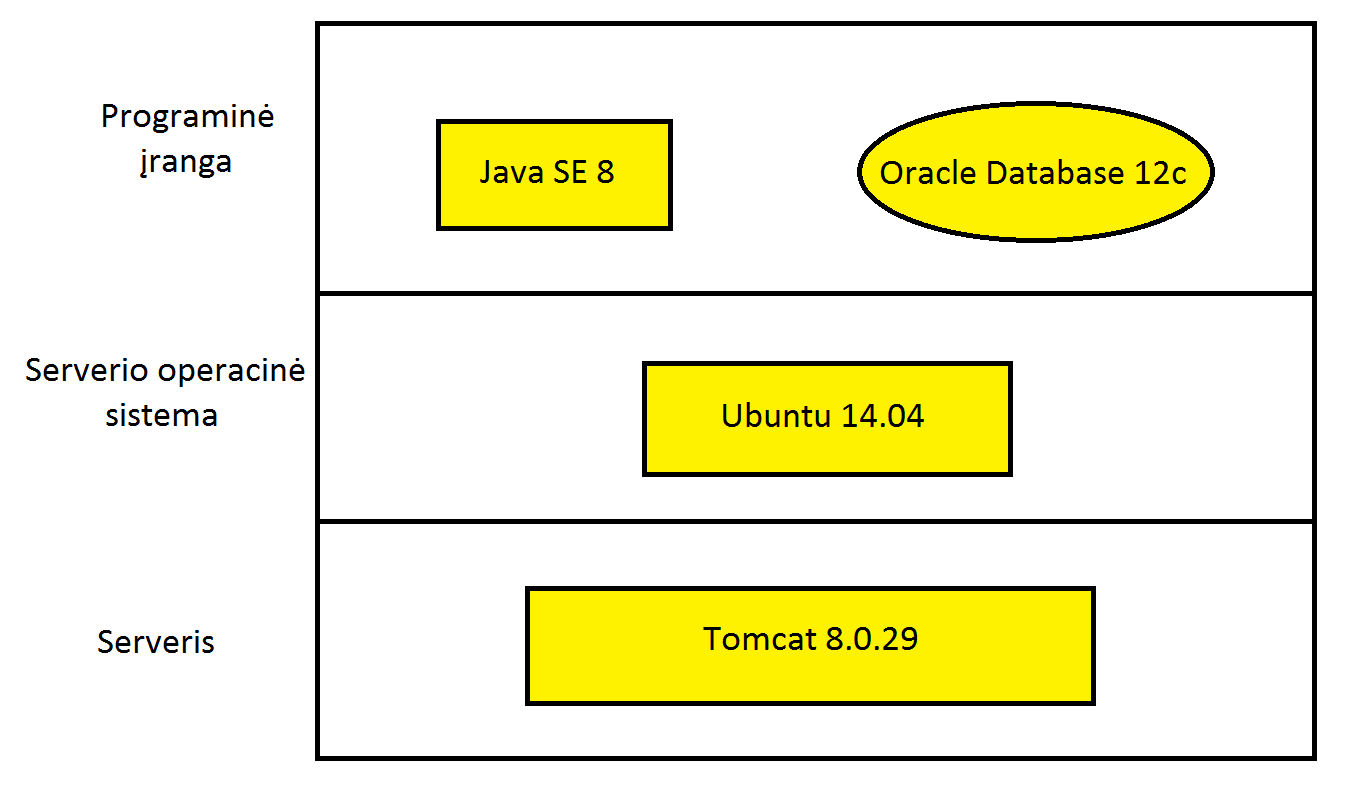
\includegraphics[scale=0.5]{architektura1}
\subsection{Sistemos komponentai}
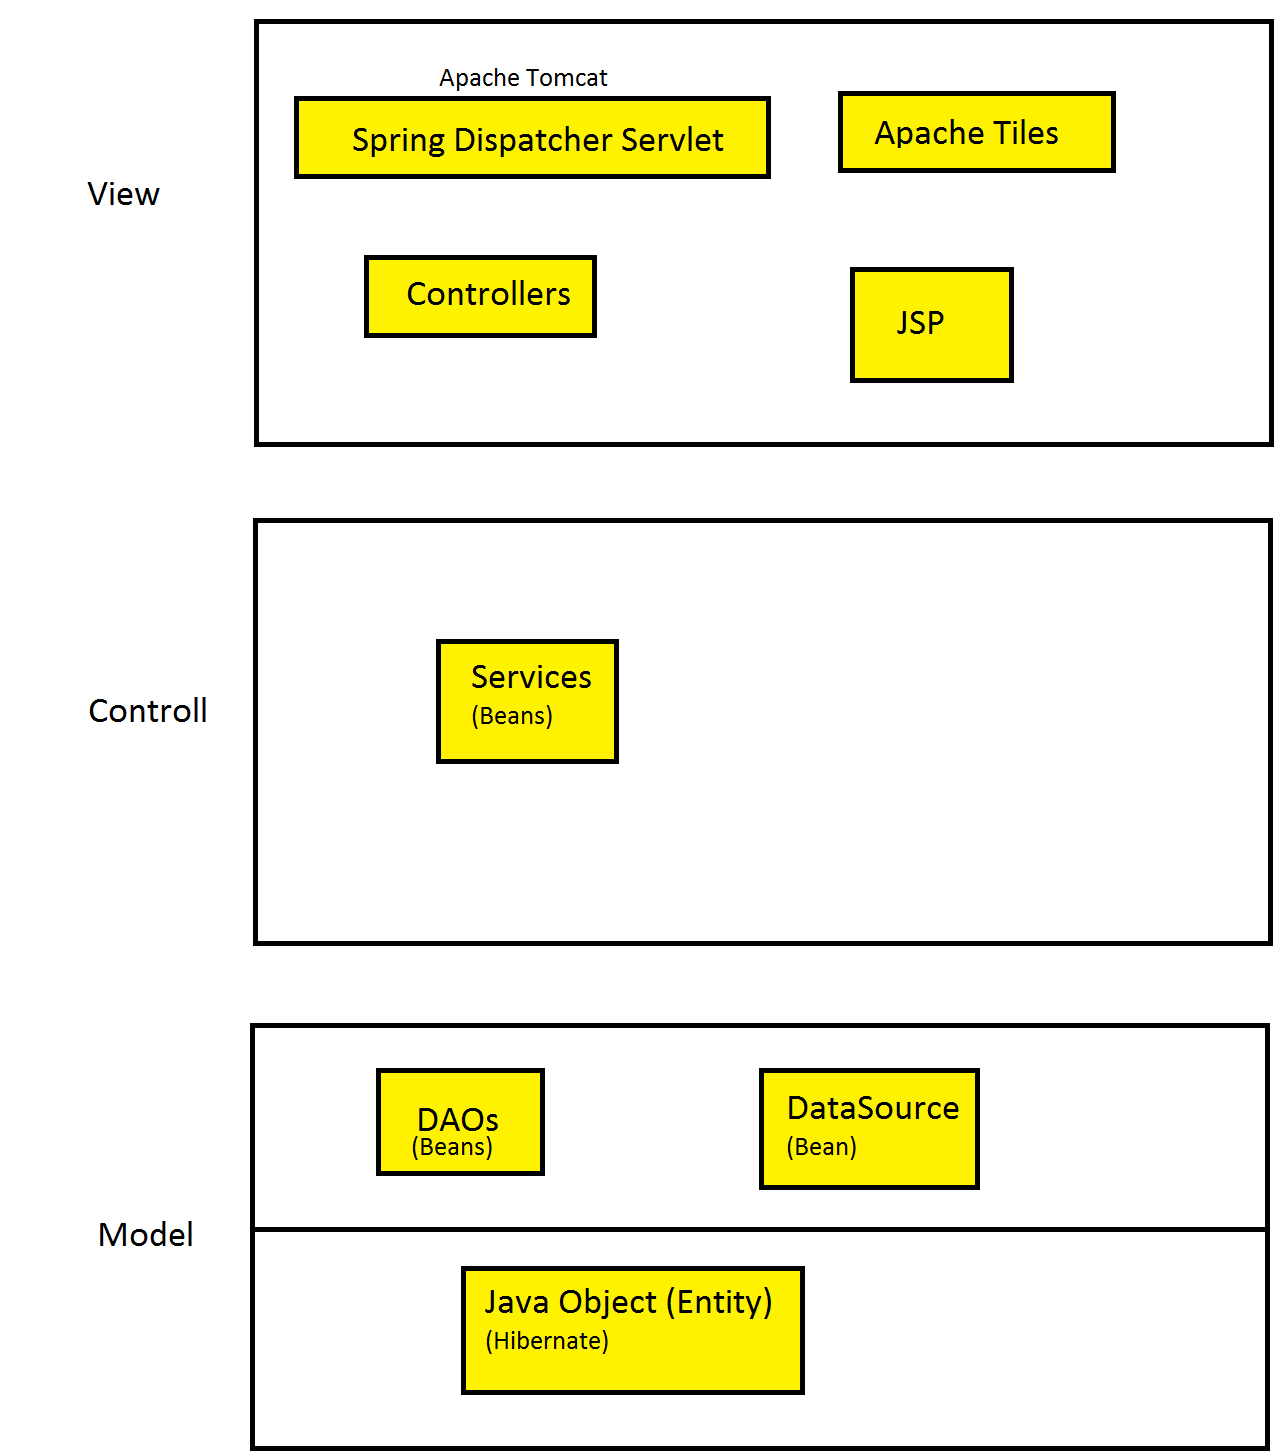
\includegraphics[scale=0.5]{architektura2}


\section{Sudėtingesnių modulių veikimo apibrėžimai}

\subsection{ Paskyros parametrų keitimas }

\subsubsection{Parametrų keitimas}
Prisijungus galima pakeisti norimus paskyros duomenis.\\
Vartotojas gali keisti savo paskyros duomenis: \\
	prisijungimo vardą, el. paštą, slaptažodį. \\\\
	
Administratoriui atidariui paskyros keitimo langą\\
atsiranda sąrašas vartotojų. Spaudžiamas vartotojo \\
keitimo mygtukas "keisti" atsiradęs paspaudus ant vartotojo.\\
Dėl duomenų saugumo administratorius gali pakeisti tik\\
vartotojų prisijungimo vardus ir prisijungimo paštus. \\\\

Pakeitimai turi atitikti registracijos formos reikalavimus: \\
	\tabitem prisijungimo vardas >= 4 simboliai\\
	\tabitem unikalus paštas bei prisijungimo vardas.
    \tabitem slaptažodis >= 8 simboliai. \\\\
    
Pakeitimai patikrinami ir jei nera klaidų tada užklausa siunčiama \\
į duomenų bazėje. Taip pat pakeisti duomenys atnaujinami administratoriaus \\
vartotojų paskyrų sąraše. \\
Jei klaidų randama - neatitinka reikalavimų tada pažymimi neleistinas \\
reikšmes įgiję laukai.\\

\subsubsection{P.O. mokestis}
P.O. mokėjimą galima atlikti po prisijungimo. \\
Vartotojas paspaudęs mokėjimo mygtuką nurodo:
\begin{itemize}
	\item Aktyvuojamo vartotojo pašto adresą.
	\item Mokėjimo laikotarpį.
	\item Datą laikotarpio pradžiai.
\end{itemize} 
Mokėjimo laikotarpiai yra mėnesis(5€) ir metai(25€). \\
Jei vartotojas - aktyvuotas, paskyroje nurodomas aktyvacijos galiojimo laikas.\\
Aktyvuotas vartotojas gali pratęsti aktyvacijos galiojimo laiką, \\
bet data turėtų būti vėlesnė už paskutinę galiojimo dieną.\\
Jei vartotojas - neaktyvuotas, tada nurodo mokėjimo laikotarpį bei datą,
ne ankstesnę už šiandieną. \\
Spaudžiamas banko mygtukas per kurį bus atliekamas atsiskaitymas.
Tinkamai atlikus pavedimą, vartotojo paskyra aktyvuojama arba aktyvacija pratęsiama.

Visų pirma patikrinamas norimas aktyvuoti paštas. \\
Jei jis neegzistuoja duomenų bazėje pranešama, kur vartotojui klaida.\\

Tikrinama ar data įvesta ne ankstesnė nei šiandienos. Jei data bloga - vartotojui pranešama, \\
kad data turi būti ne ankstesnė nei šiandienos.

Toliau su dar viena užklausa db. gaunama data paskutinės galiojimo datos jei tokia yra. \\
Jei nėra vykdomas mokėjimas. \\
Jei paskutinė galiojimo data yra ankstesnė nei nurodyta mokėjimo formoje mokėjimas nevyksta, \\
pranešama paskutinė aktyvacijos galiojimo dienos data. Kitu atveju vykdomas mokėjimas. \\

Po sekmingai ivykdyto mokėjimo vartotojo būsena pakeičiama į aktyvuotą.
 
	
	
\subsection{ P.O. duomenų įvedimas }

Prie panelių įvedimo duotos dvi pasirenkamos standartinės panelės 1200x2500 ir 1200x3050\\ 
dydžių bei papildomos reikiamų matmenų panelės įvedimas, bei mygtukas "Pridėti naują", \\
kurį paspaudus atsiranda dar vienas papildomos panelės įvedimas, jei bendra panelių suma \\
neviršija dešimties. \\
Detales galima įvesti rankiniu budu bei importuoti ".csv" formatu. 
Taip pat yra mygtukas "Parsisiūsti importuojamo failo pavyzdį", skirtas atsiūsti \\
pavizdinį ".csv" failą, kuriame parodoma kaip reikia suvesti detales į tokį failą. \\
Mygtukas "Istorija" parodo sąrašą išsaugotų pjovimo optimizacijos planų.

\subsubsection{Duomenų validavimas}
\textbf{Tikrinamas standartinių panelių validumas}:\\
	Tikrinama ar yra pasirinkta bent viena panelė. \\
	Toliau tikrinama ar pasirinktų panelių ilgai ir pločiai nuo 10mm iki 10000mm \\


\textbf{Tikrinamas detalių validumas}:\\
	Surandama iš pasirinktų panelių mažiausias ilgis bei plotis .\\
	Tada tikrinama ar detalės ilgis ir plotis mažesnis ar lygus už rastus mažiausius ilgius, pločius.\\
	Tikrinama ar detalių bendaras kiekis neviršija 1000000. \\

Jei validavimas teisingas vykdoma pjovimo optimizacija.

\subsubsection{Detalių .csv failo validavimas}
\textbf{Tikrinamas detalių validumas}:\\
	Pirmiausiai patikrinama ar failas csv formato. \\
	Kekvienoje eilutėje turi būti 3 duomenys perskirti kableliais, Jei formatas netinka 
	išvedamas pranešimas "netinkamas formatas". \\
	Pirmas nurodomas detalės kiekis nuo 1 iki 1000000, antras ilgis ir trečias plotis. \\
	Ilgis, plotis turi atitikti detalių validumo standartus, sudėtinis kiekis neviršija 1000000.\\
	


\subsubsection{Duomenų susiejimas}





\subsection{ Pjūvio plano informacijos išsaugojimas bei "Istorijos" mygtukas}
\subsubsection{Pjūvio plano informacijos išsaugojimas}
Duomenų įvedimo skilty išsaugomas paskutinį kartą įvesti pakeisti duomenys.\\
Sekantį sykį vartotojui atidarius duomenų skilty įvedime bus paskutinį kartą vartotojo vesti duomenys.

Pasirinkęs reikalinga ruošinį vartotojui pateikiamas mygtukas išsaugoti duomenys. \\
Paspaudus jį pateikiamas plano pavadinimo įvedimas, kuriuo bus saugomi duomenys. \\
Paspaudžiamas mygtukas saugoti. \\
Plano pavadinimas įkeliamas į mygtuko "Istorija" sąraše jei dar nėra 10 ruošinių.\\
Kitu atveju atsiranda pranešimas: \\
"Jūsų istorijoje jau yra saugoma 10 įrašų. Uždarykite įš langelį ir istorijoje pašalinkite vieną iš įrašų, kad galėtumėte išsaugoti šitą planą". \\

\subsubsection{"Istorijos" mygtukas}
Istorijos saraše naujiausi planai išsaugoti-aukščiausiai, seniausi išsaugoti žemiausiai.
Prie plano pavadinimo seka data bei 5 to plano panaudojimo mygtukai.\\
Paspaudus mygtuką "Naudoti duomenis" nukeliama į duomenų skilty.
Ten jau suvesti pasirinkto plano duomenys.

Paspaudus mygtuką "Peržiūrėti planą" pateikiami išsaugoti rezultatai:\\
detalių išdėstymas, sunaudotas panelių kiekis, bendras jų plotas, likutis, bendras pjovimo ilgis.

Paspaudus atsisiuntimo formos mygtuką atsiunčiami minėti duomenys ".pdf" formatu.\\
Paspaudus šiukšliadežės formos mygtuką ištrinamas išsaugotas planas.\\
Paspaudus "floppy disk" formos mygtuką išsaugomas pakeistas plano pavadinimas.

\clearpage

\section{Interfeisai}

\subsection{Pastabos}
Interfeisuose matomas geltono kontūro langas yra vadinamasis "pop-up" langas. Jo veikimo pavyzdys galėtų būti toks: paprastas vartotojas prisijungia prie savo paskyros lango, jame mato mygtuką "Mokėti", vartotojui paspaudus šį mygtuką paskyros lango turinys yra paslepiamas ir atsiranda geltono kontūro mokėjimo dialogas. Šiame dialoge esantis "X" mygtukas raudoname fone leidžia vartotojui matyti paslėptąjį turinį (su visa jame prieš tai buvusia informacija) ir, žinoma, uždario geltoname kontūre buvusį dialogą, užmirštant visą jame buvi įvestą turinį.\\
Atsijungimo mygtukas matomas tik prisijungus. O jį paspaudus, vartotojas nukreipiamas į namų puslapio langą.

\subsection{Namų puslapis}
\floatfoot{1 interfeisas. Namų puslapis (vartotojas prisijungęs)}
\begin{figure}[!tph]
\hspace{-2cm}
\centering
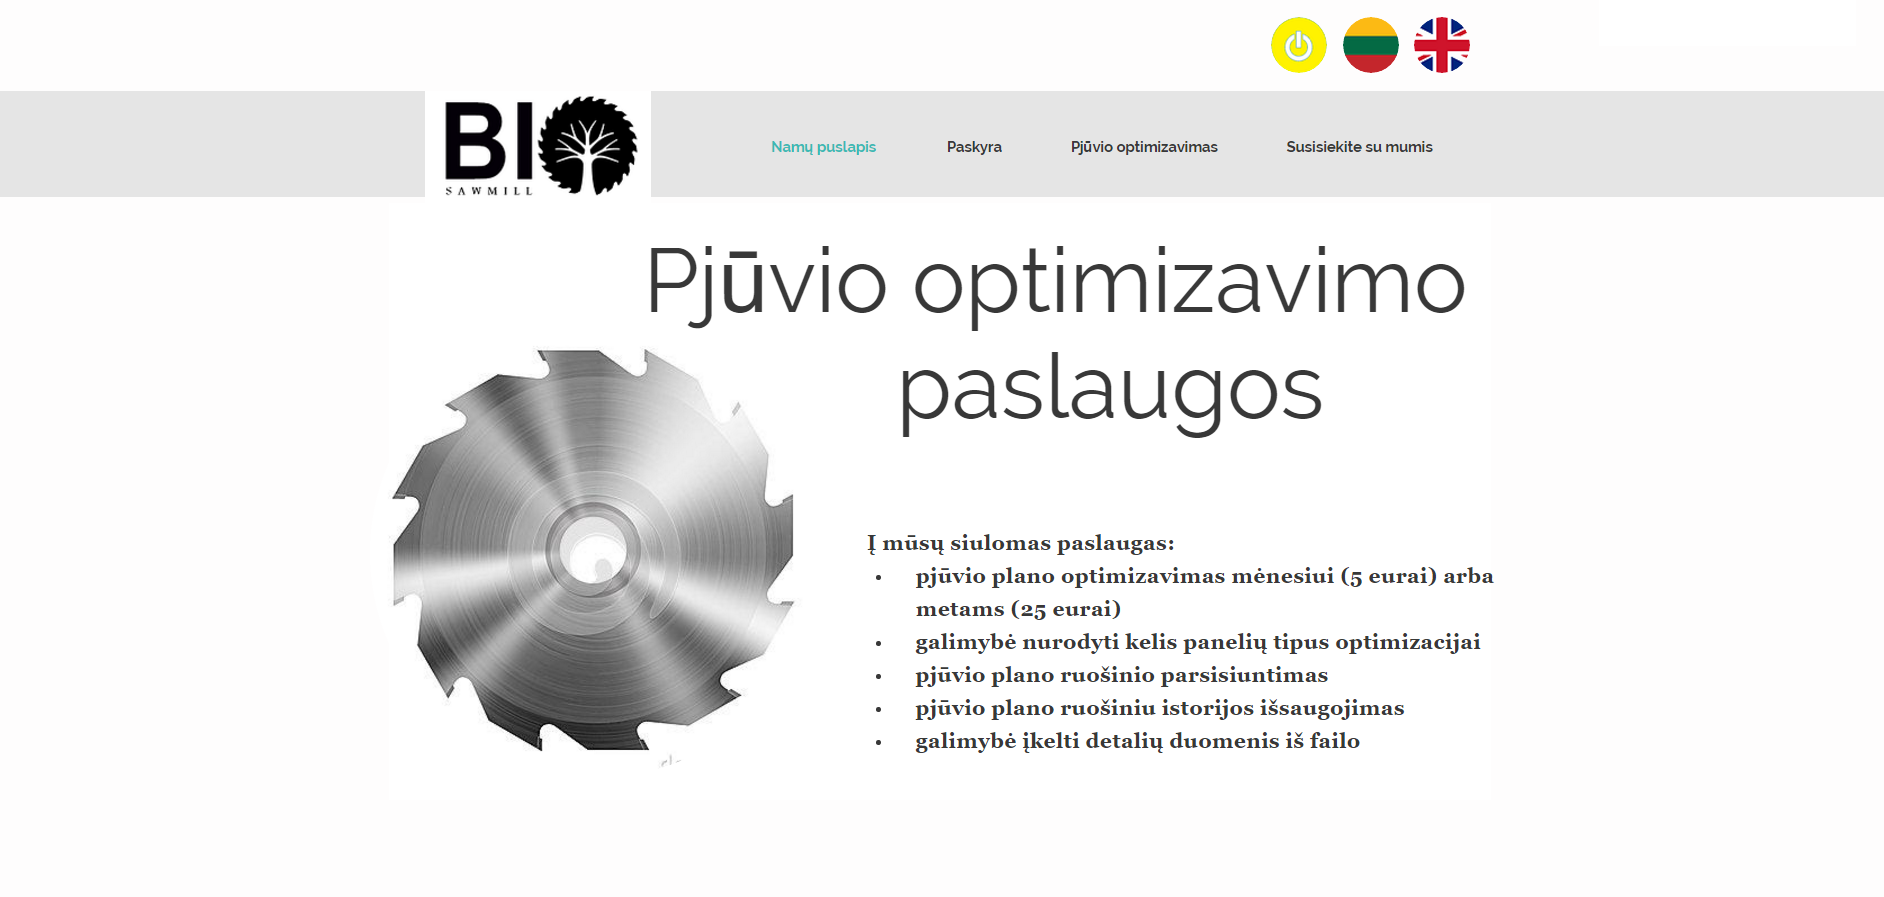
\includegraphics[scale=0.45]{interfeisai/pagrindinis}
\label{fig:verticalcell}
\end{figure}

\subsection{Vartotojo paskyros puslapis}
\floatfoot{2 interfeisas. Vartotojo paskyros puslapis}
\begin{figure}[!tph]
\hspace{-2cm}
\centering
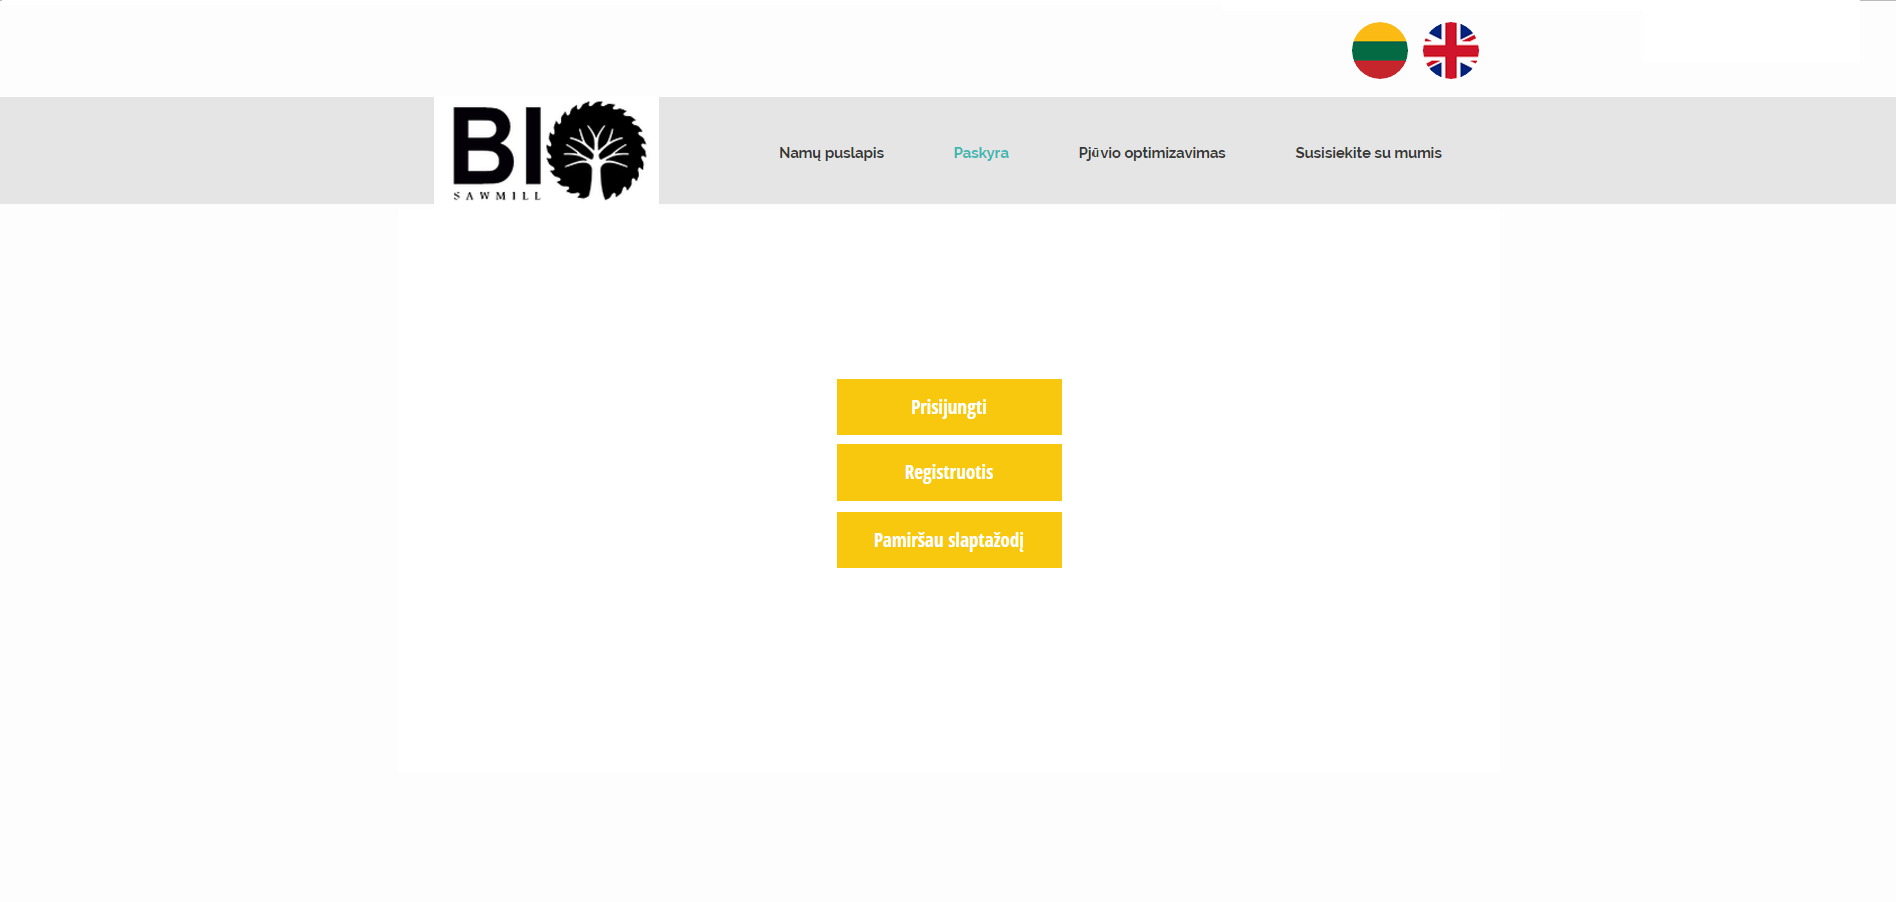
\includegraphics[scale=0.45]{interfeisai/paskyrosPuslapisNeprisijungta}
\label{fig:verticalcell}
\end{figure}

\floatfoot{3 interfeisas. Vartotojo paskyros puslapis - registracija}
\begin{figure}[!tph]
\hspace{-2cm}
\centering
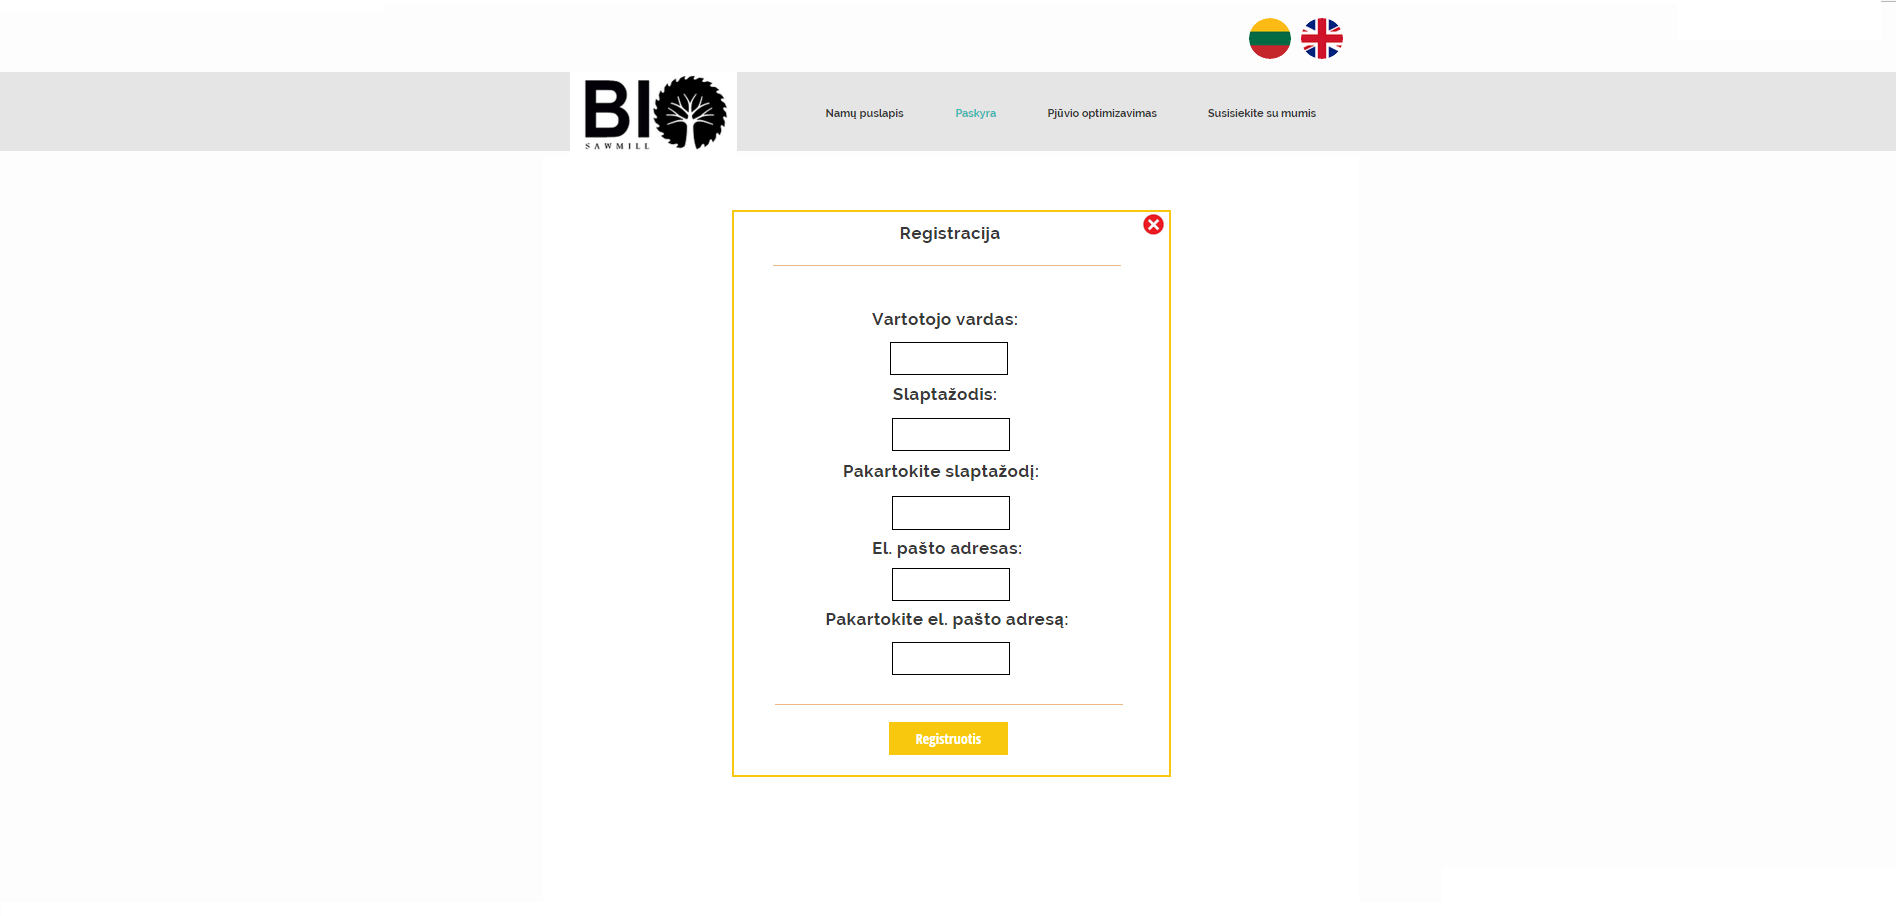
\includegraphics[scale=0.45]{interfeisai/paskyrosPuslapisRegistracija}
\label{fig:verticalcell}
\end{figure}

\floatfoot{4 interfeisas. Vartotojo paskyros puslapis - registracija (su klaida)}
\begin{figure}[!tph]
\hspace{-2cm}
\centering
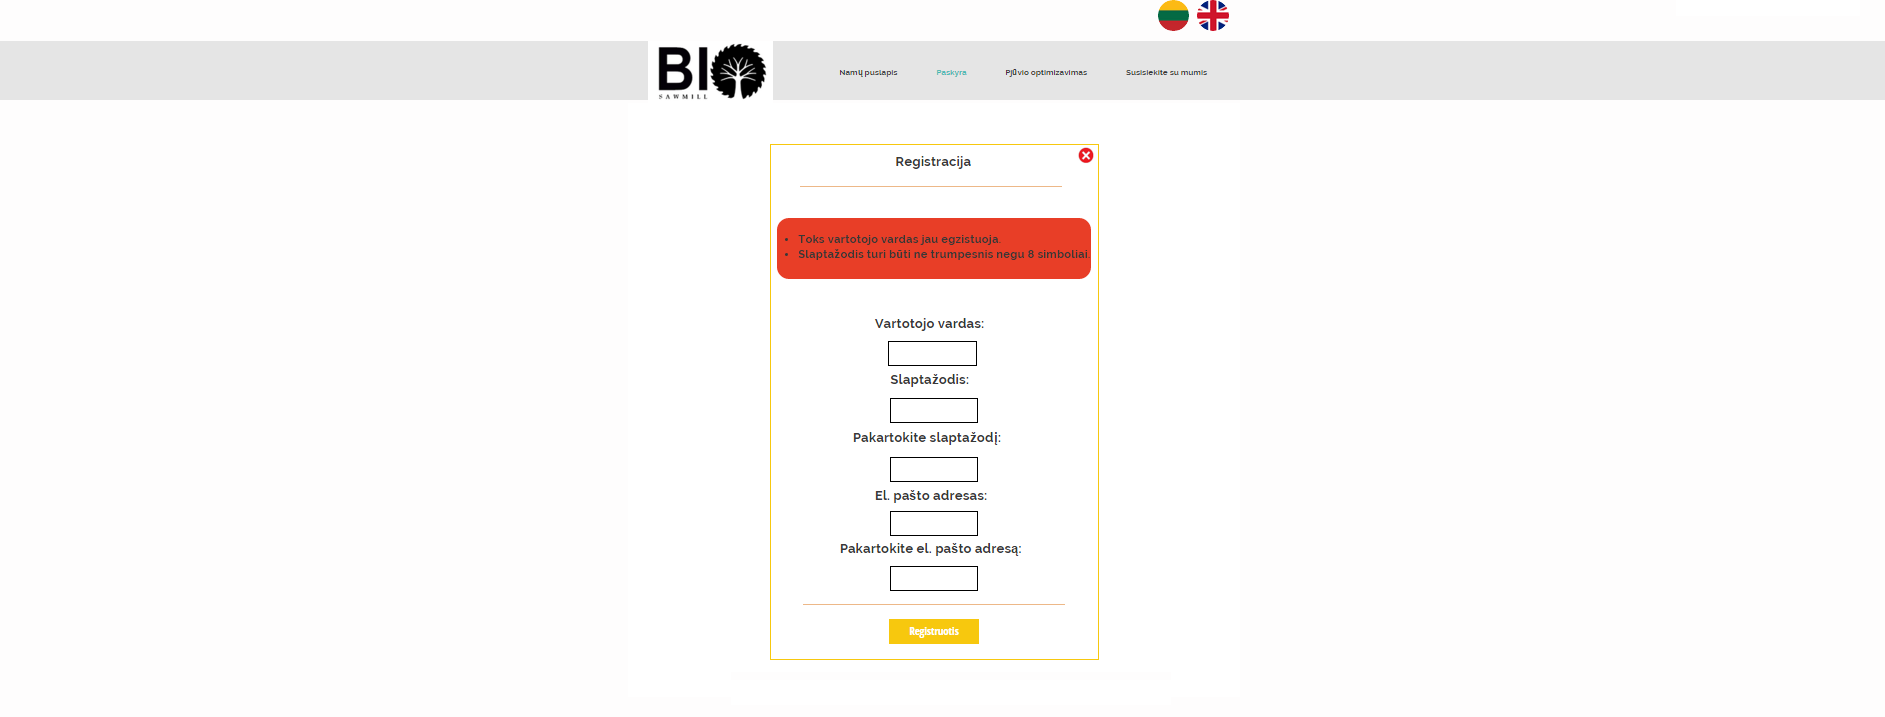
\includegraphics[scale=0.45]{interfeisai/paskyrosPuslapisRegistracijaSuKlaida}
\label{fig:verticalcell}
\end{figure}

\floatfoot{5 interfeisas. Vartotojo paskyros puslapis - sėkminga registracija}
\begin{figure}[!tph]
\hspace{-2cm}
\centering
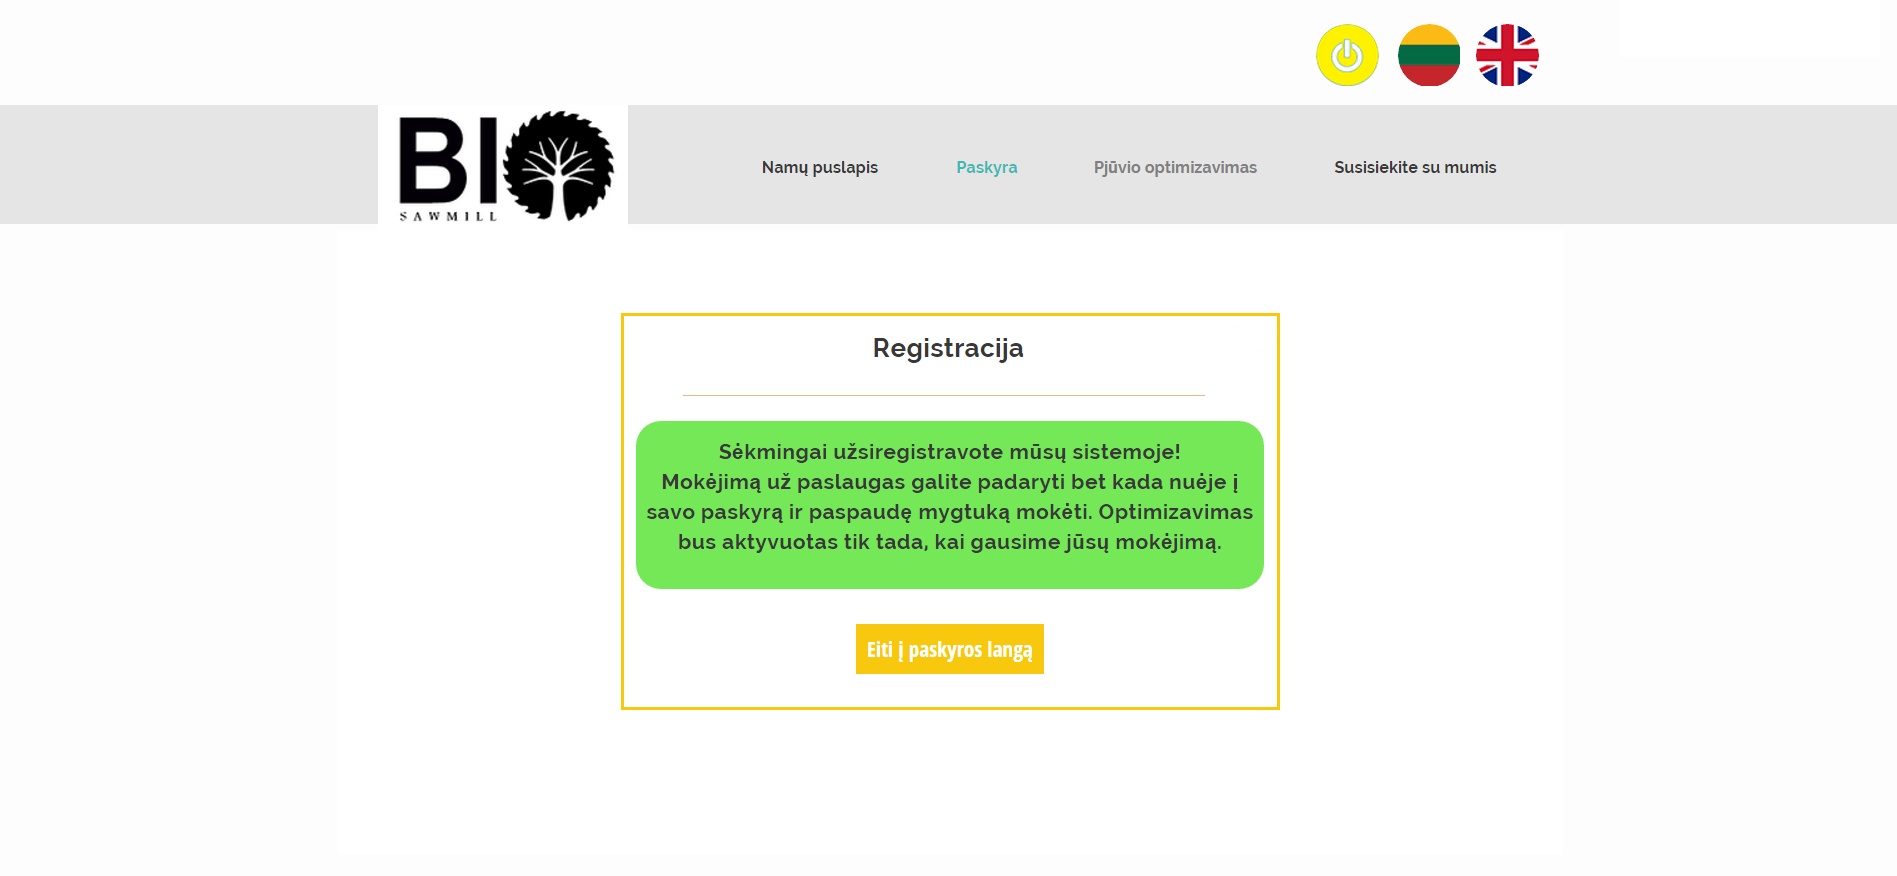
\includegraphics[scale=0.45]{interfeisai/paskyrosPuslapisRegistracijaSekminga}
\label{fig:verticalcell}
\end{figure}
 
\floatfoot{6 interfeisas. Vartotojo paskyros puslapis - prisijungimas. Sėkmingai prisijungus, vartotojas nukreipiamas į 10 arba 11 interfeisą, priklauso nuo to ar jis yra užsimokėjęs už paslaugas.}
\begin{figure}[!tph]
\hspace{-2cm}
\centering
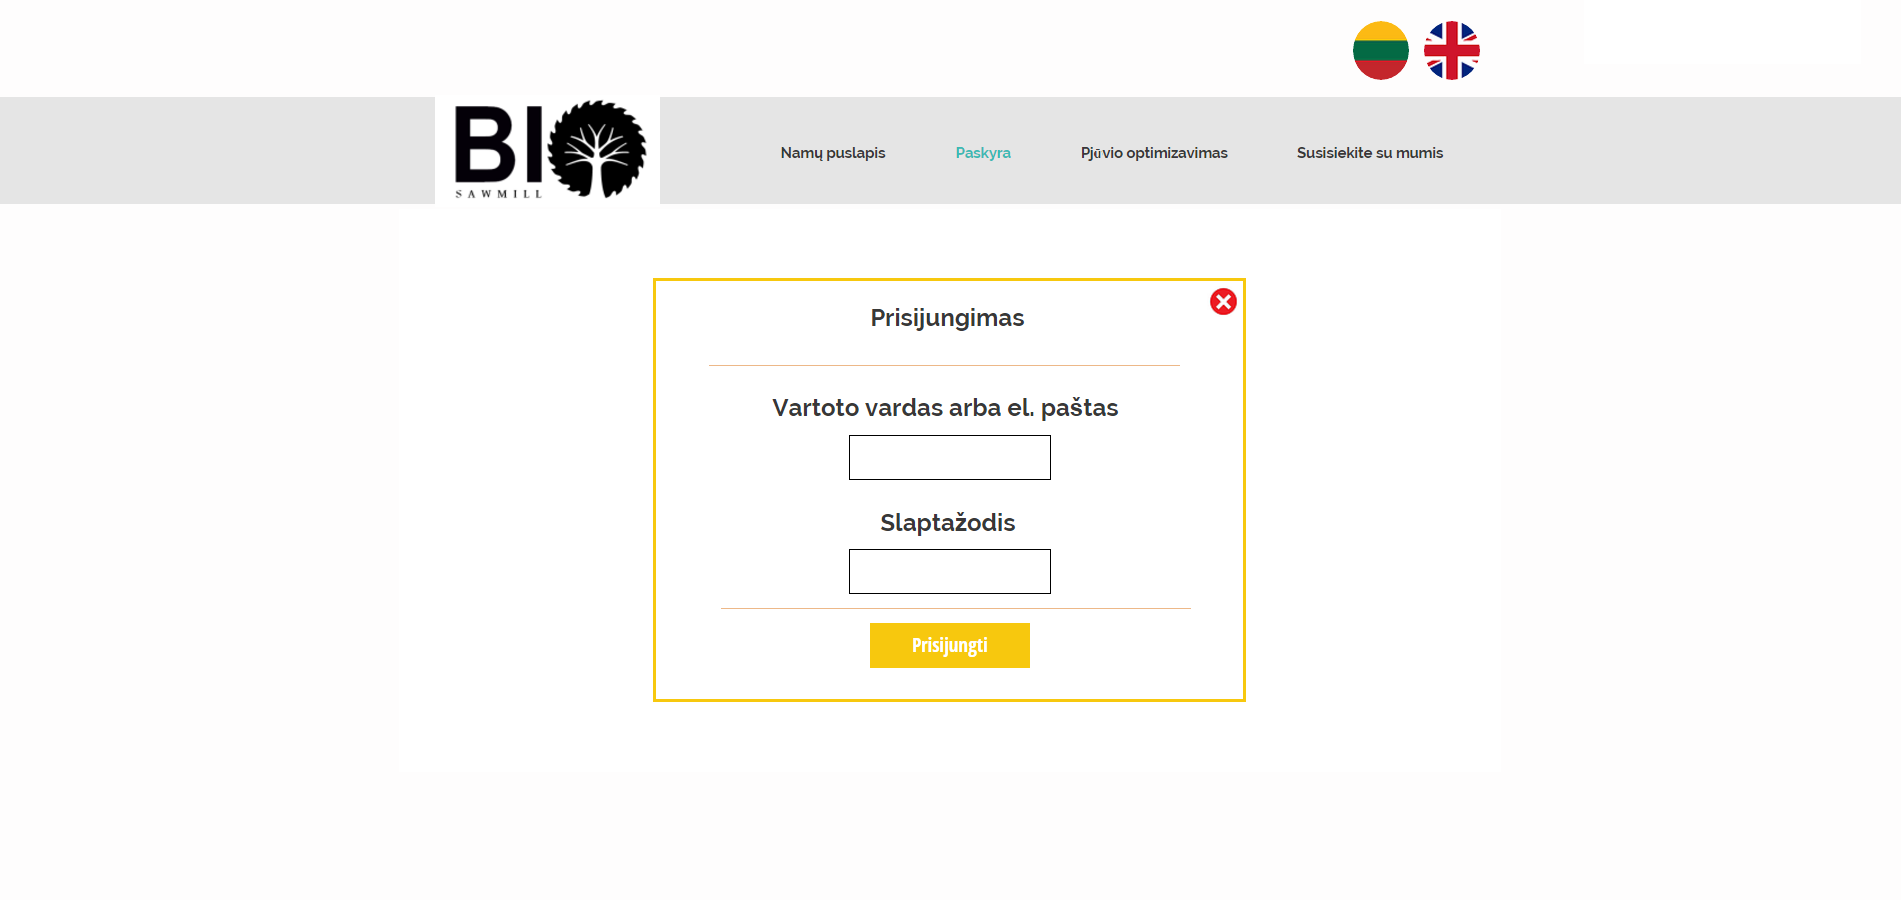
\includegraphics[scale=0.45]{interfeisai/paskyrosPuslapisPrisijungimas}
\label{fig:verticalcell}
\end{figure}

\floatfoot{7 interfeisas. Vartotojo paskyros puslapis - prisijungimas (su klaida)}
\begin{figure}[!tph]
\hspace{-2cm}
\centering
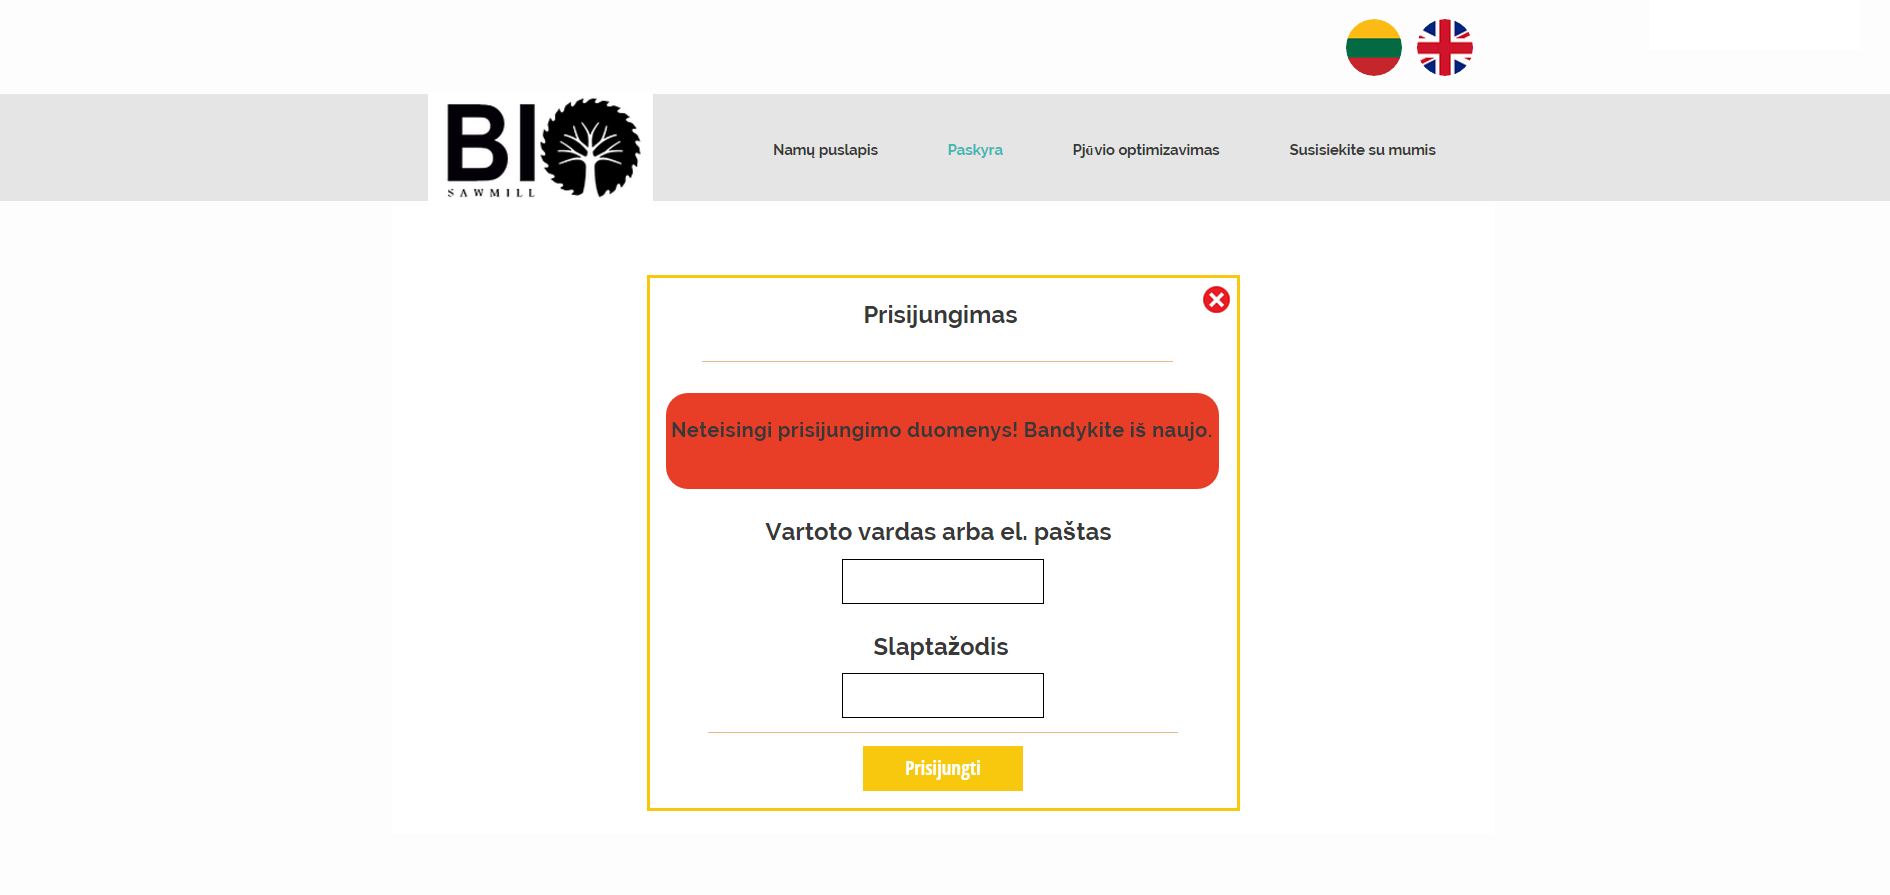
\includegraphics[scale=0.45]{interfeisai/paskyrosPuslapisPrisijungimasSuKlaida}
\label{fig:verticalcell}
\end{figure}

\floatfoot{8 interfeisas. Vartotojo paskyros puslapis - pamirštas slaptažodis. Vartotojui paspaudus "Priminti slaptažodį" jis nukreipiamas į 9 interfeisą.}
\begin{figure}[!tph]
\hspace{-2cm}
\centering
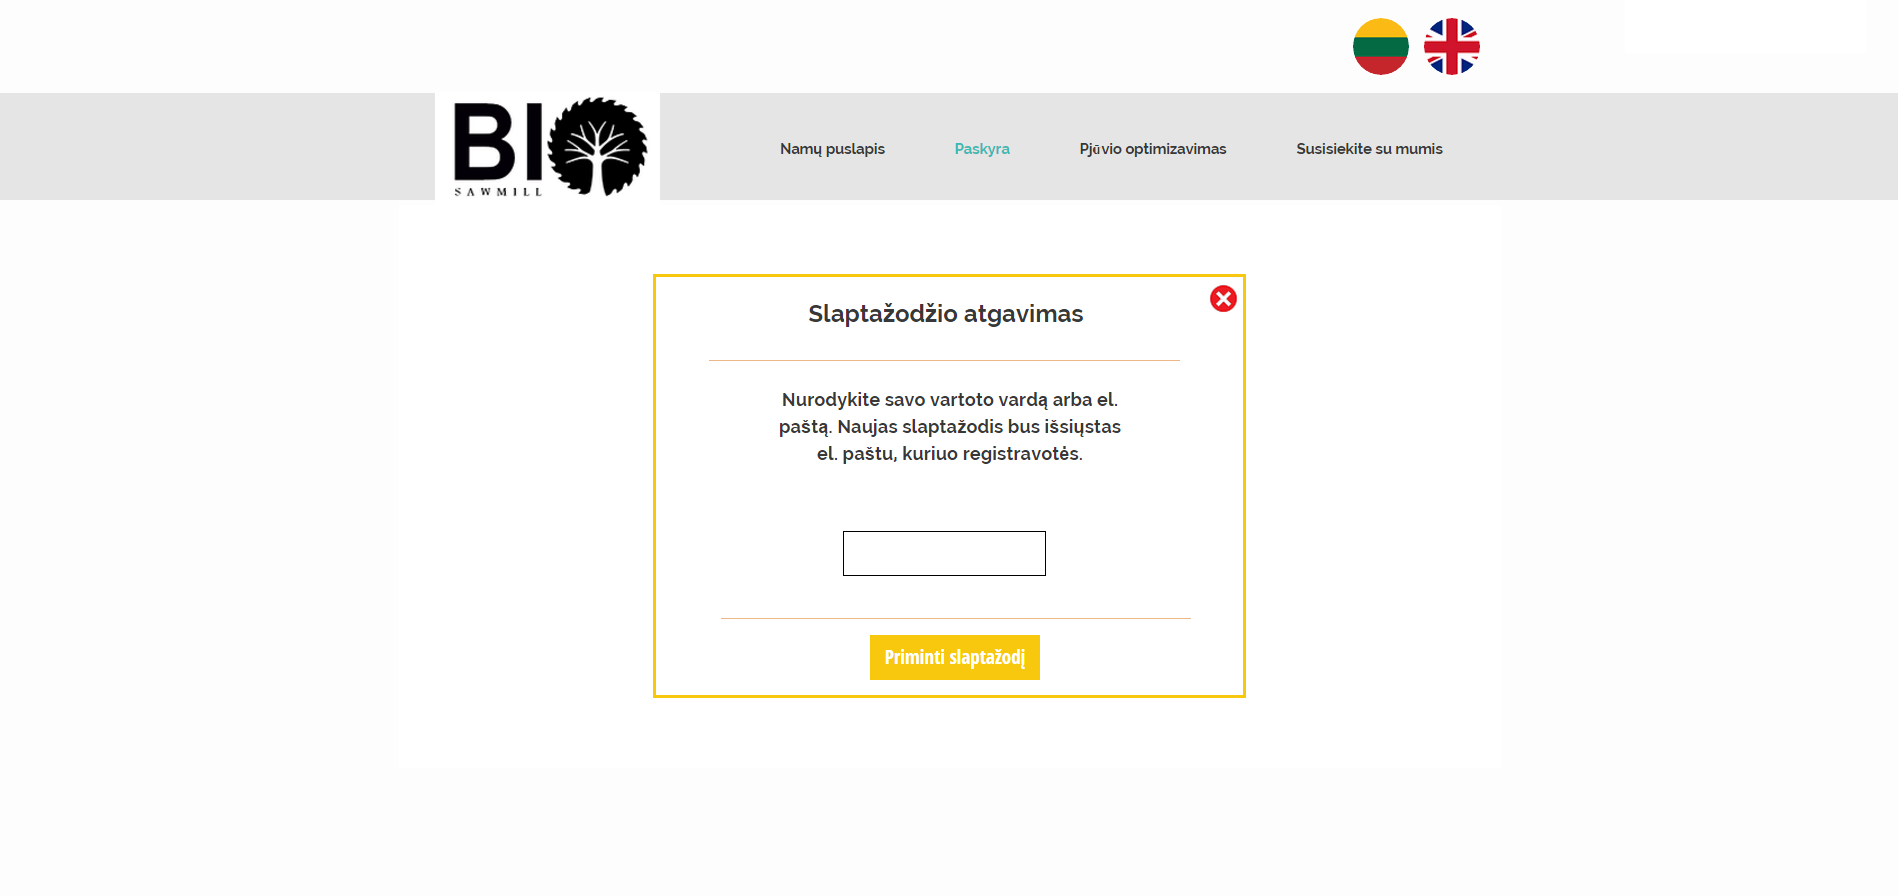
\includegraphics[scale=0.45]{interfeisai/paskyrosPuslapisPamirstasSlaptazodis}
\label{fig:verticalcell}
\end{figure}

\floatfoot{9 interfeisas. Vartotojo paskyros puslapis - pamirštas slaptažodis 2. Vartotojui paspaudus "X" jis yra gražinamas į 2 interfeisą. Vartotojui paspaudus "Bandyti dar kartą" jis yra gražinamas į 8 interfeisą.}
\begin{figure}[!tph]
\hspace{-2cm}
\centering
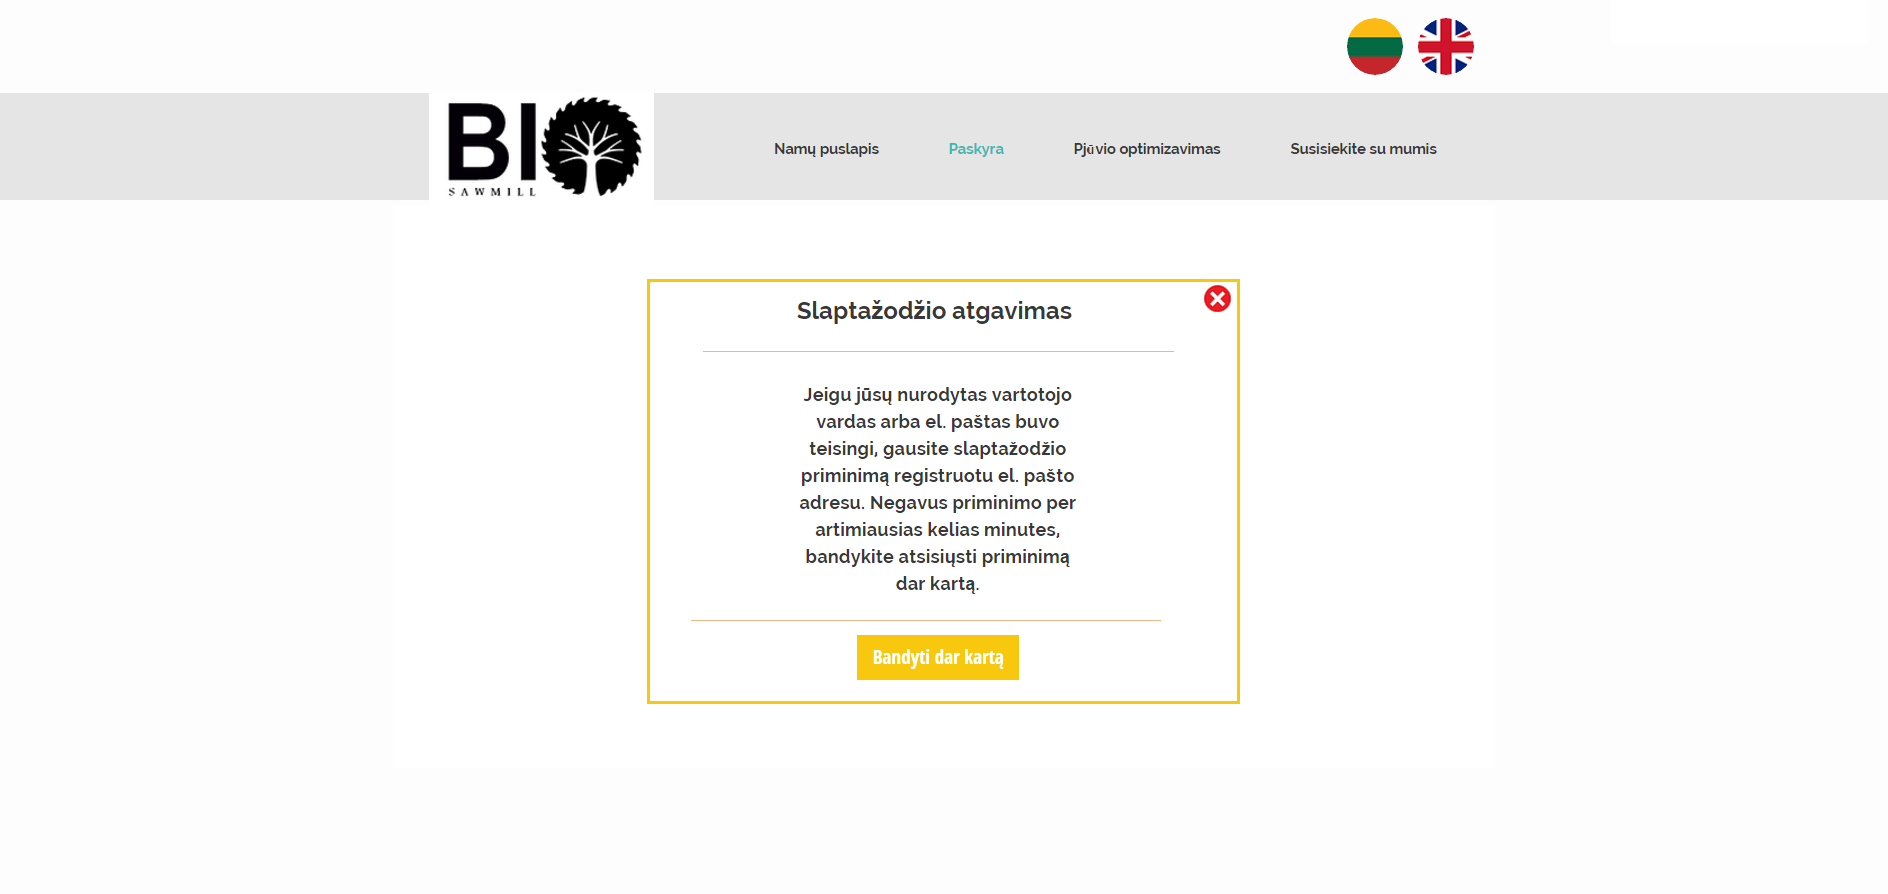
\includegraphics[scale=0.45]{interfeisai/paskyrosPuslapisPamirstasSlaptazodis2}
\label{fig:verticalcell}
\end{figure}


\floatfoot{10 interfeisas. Vartotojo paskyros puslapis - prisijungus (neapmokėta už paslaugas)}
\begin{figure}[!tph]
\hspace{-2cm}
\centering
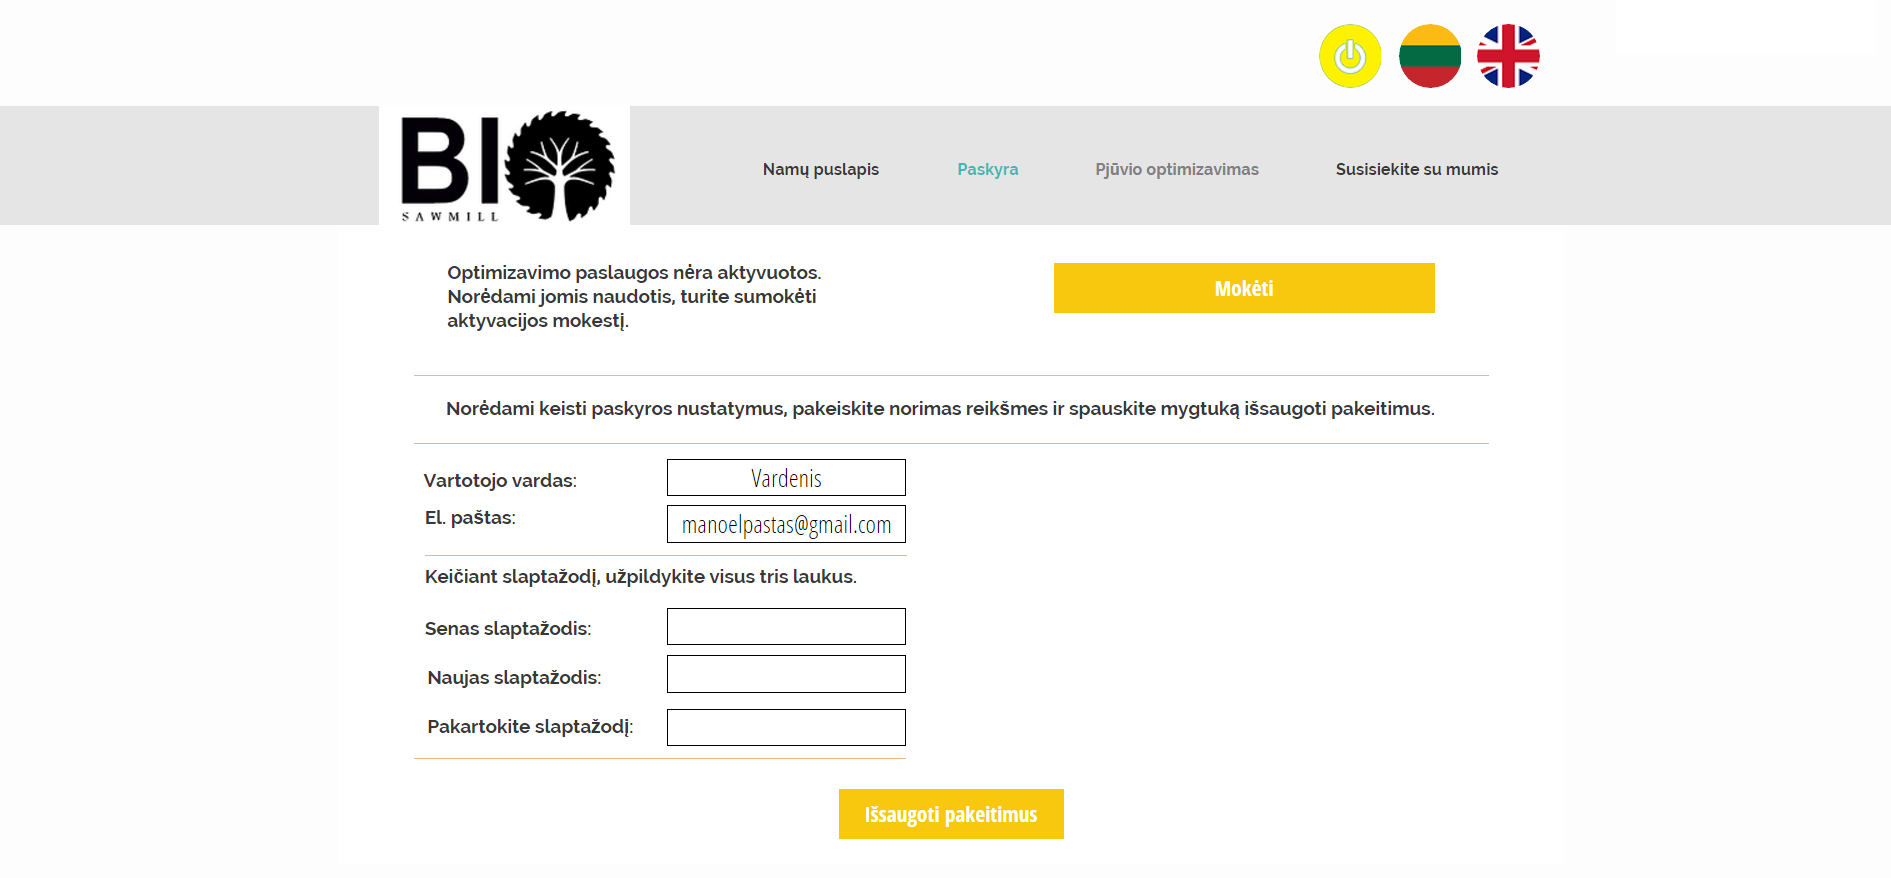
\includegraphics[scale=0.45]{interfeisai/paskyrosPuslapisVartotojasNeapmoketas}
\label{fig:verticalcell}
\end{figure}

\floatfoot{11 interfeisas. Vartotojo paskyros puslapis - prisijungus (apmokėta už paslaugas)}
\begin{figure}[!tph]
\hspace{-2cm}
\centering
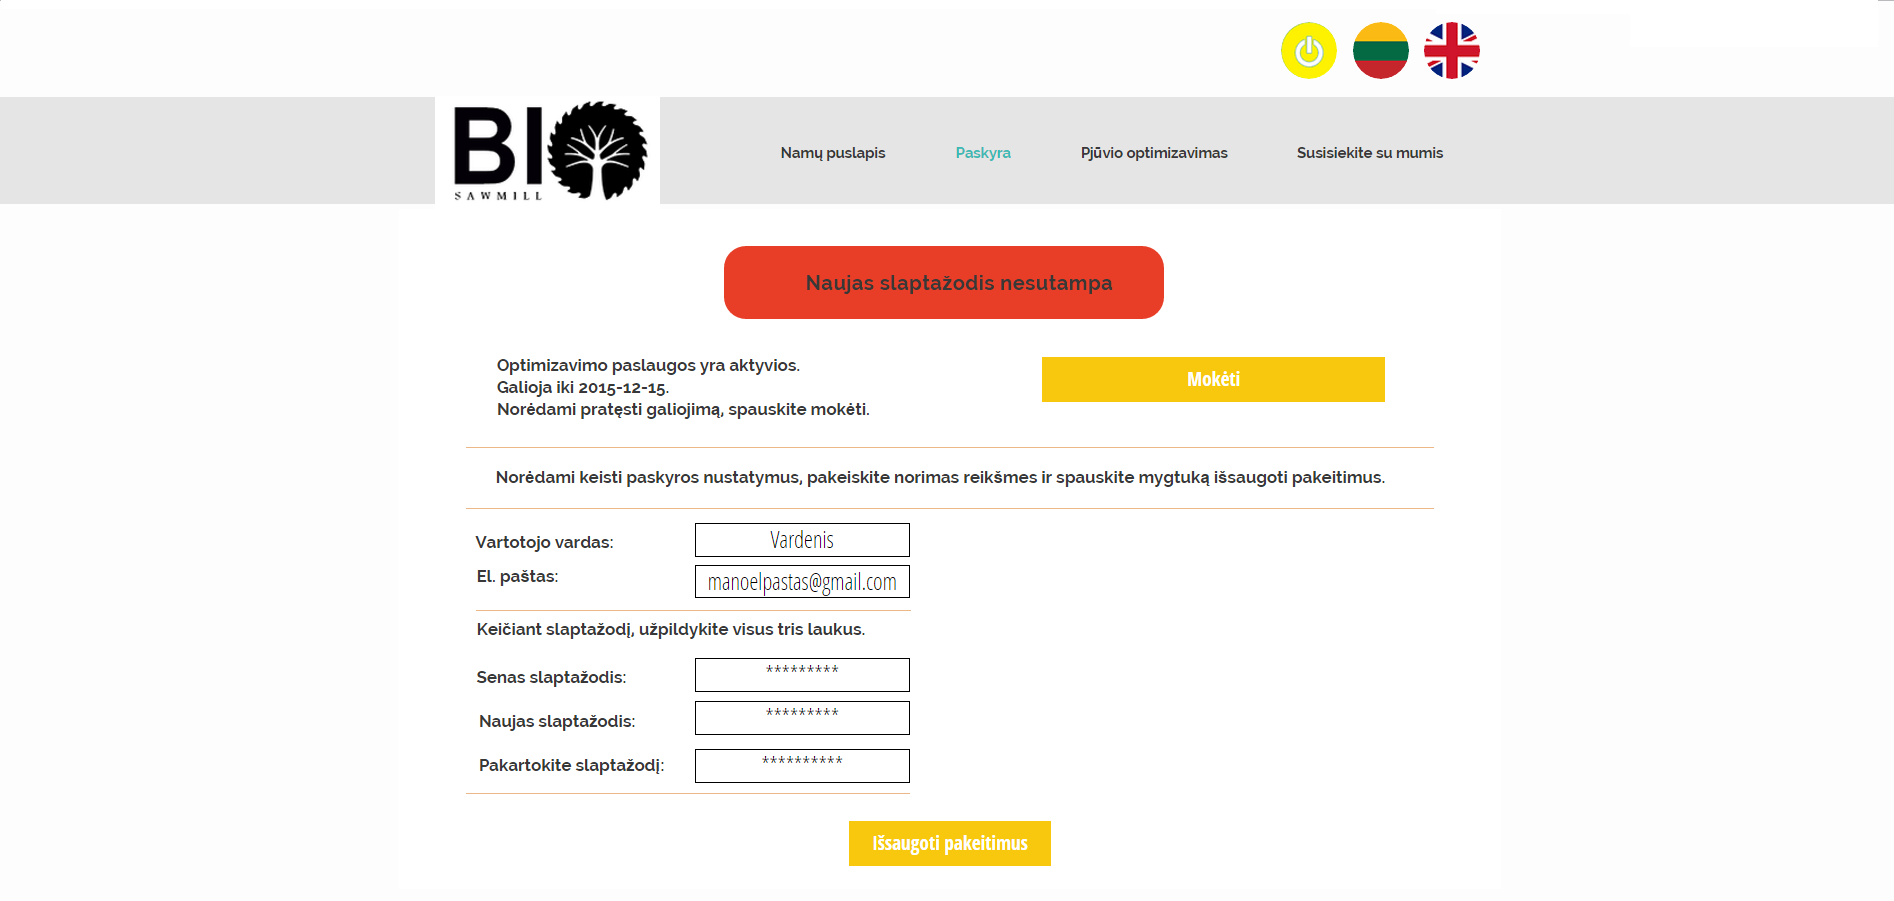
\includegraphics[scale=0.45]{interfeisai/paskyrosPuslapisVartotojasApmoketas}
\label{fig:verticalcell}
\end{figure}

\floatfoot{12 interfeisas. Vartotojo paskyros puslapis - prisijungus - mokėjimas. Įvykus sėkmigam apmokėjimui, mokėjimo langas dingsta, vartotojui gražinamas paskyros lango turinys, tačiau turinys yra nebe 10, o 11 interfeiso dizaino tipo.}
\begin{figure}[!tph]
\hspace{-2cm}
\centering
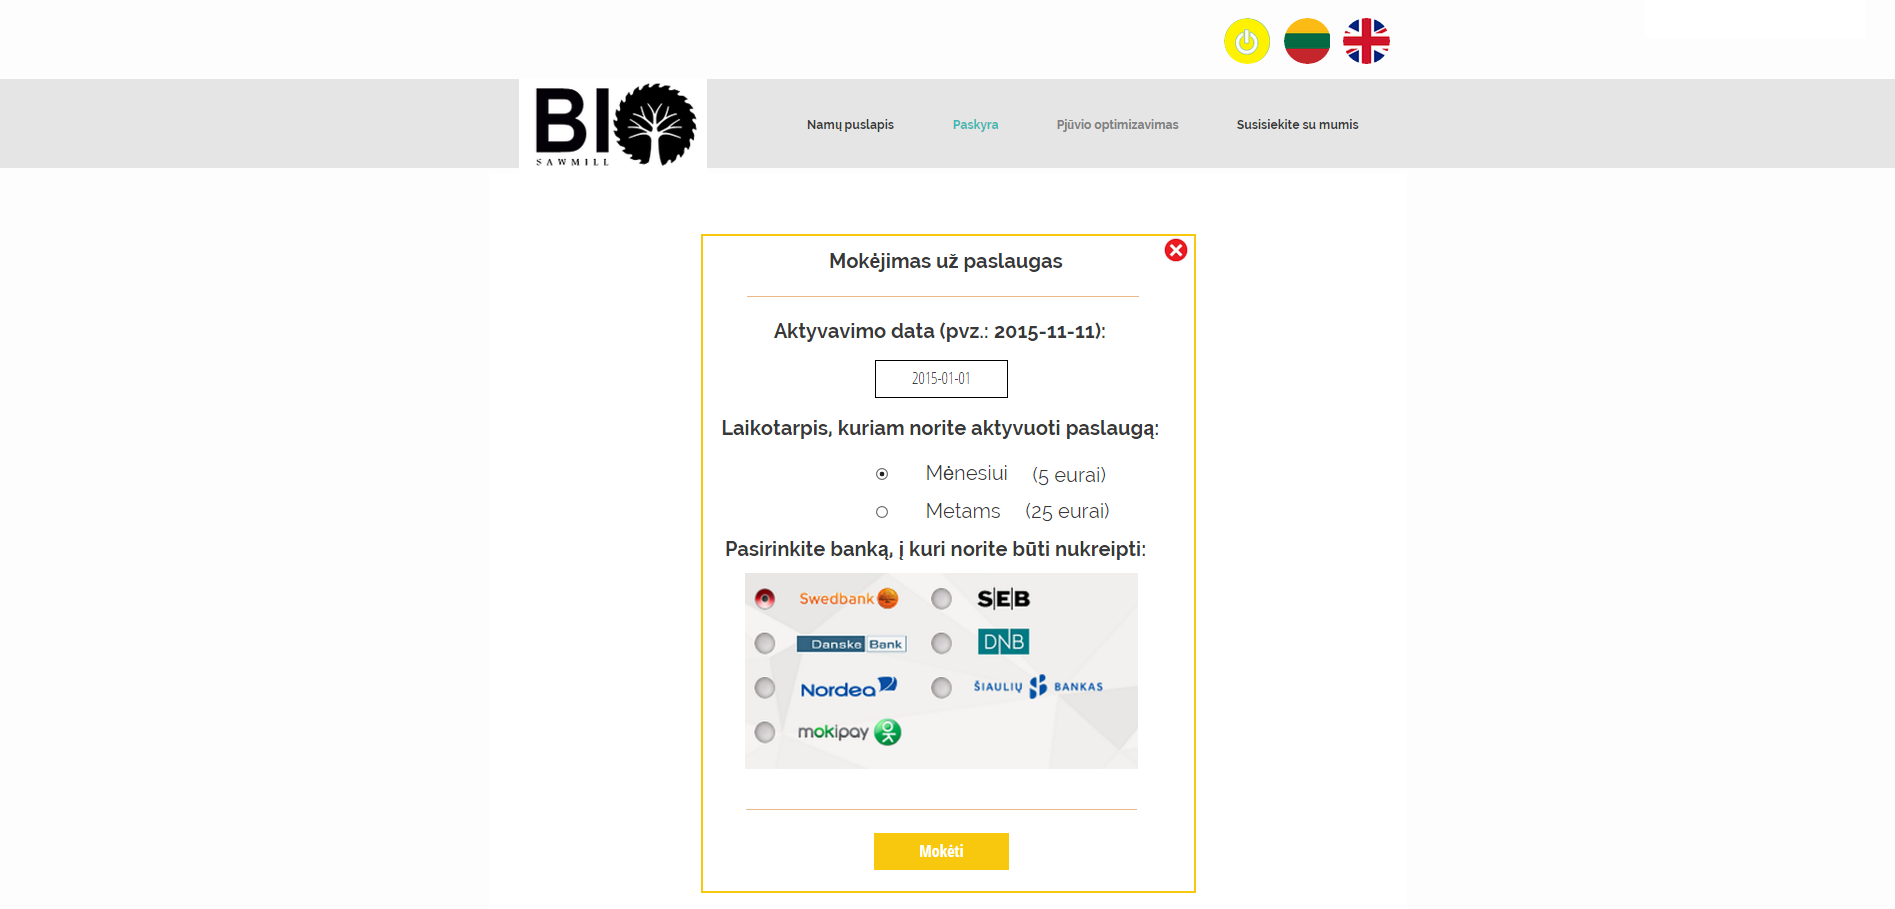
\includegraphics[scale=0.45]{interfeisai/paskyrosPuslapisVartotojasMokejimas}
\label{fig:verticalcell}
\end{figure}

\floatfoot{13 interfeisas. Vartotojo paskyros puslapis - prisijungus - mokėjimas (su klaida)}
\begin{figure}[!tph]
\hspace{-2cm}
\centering
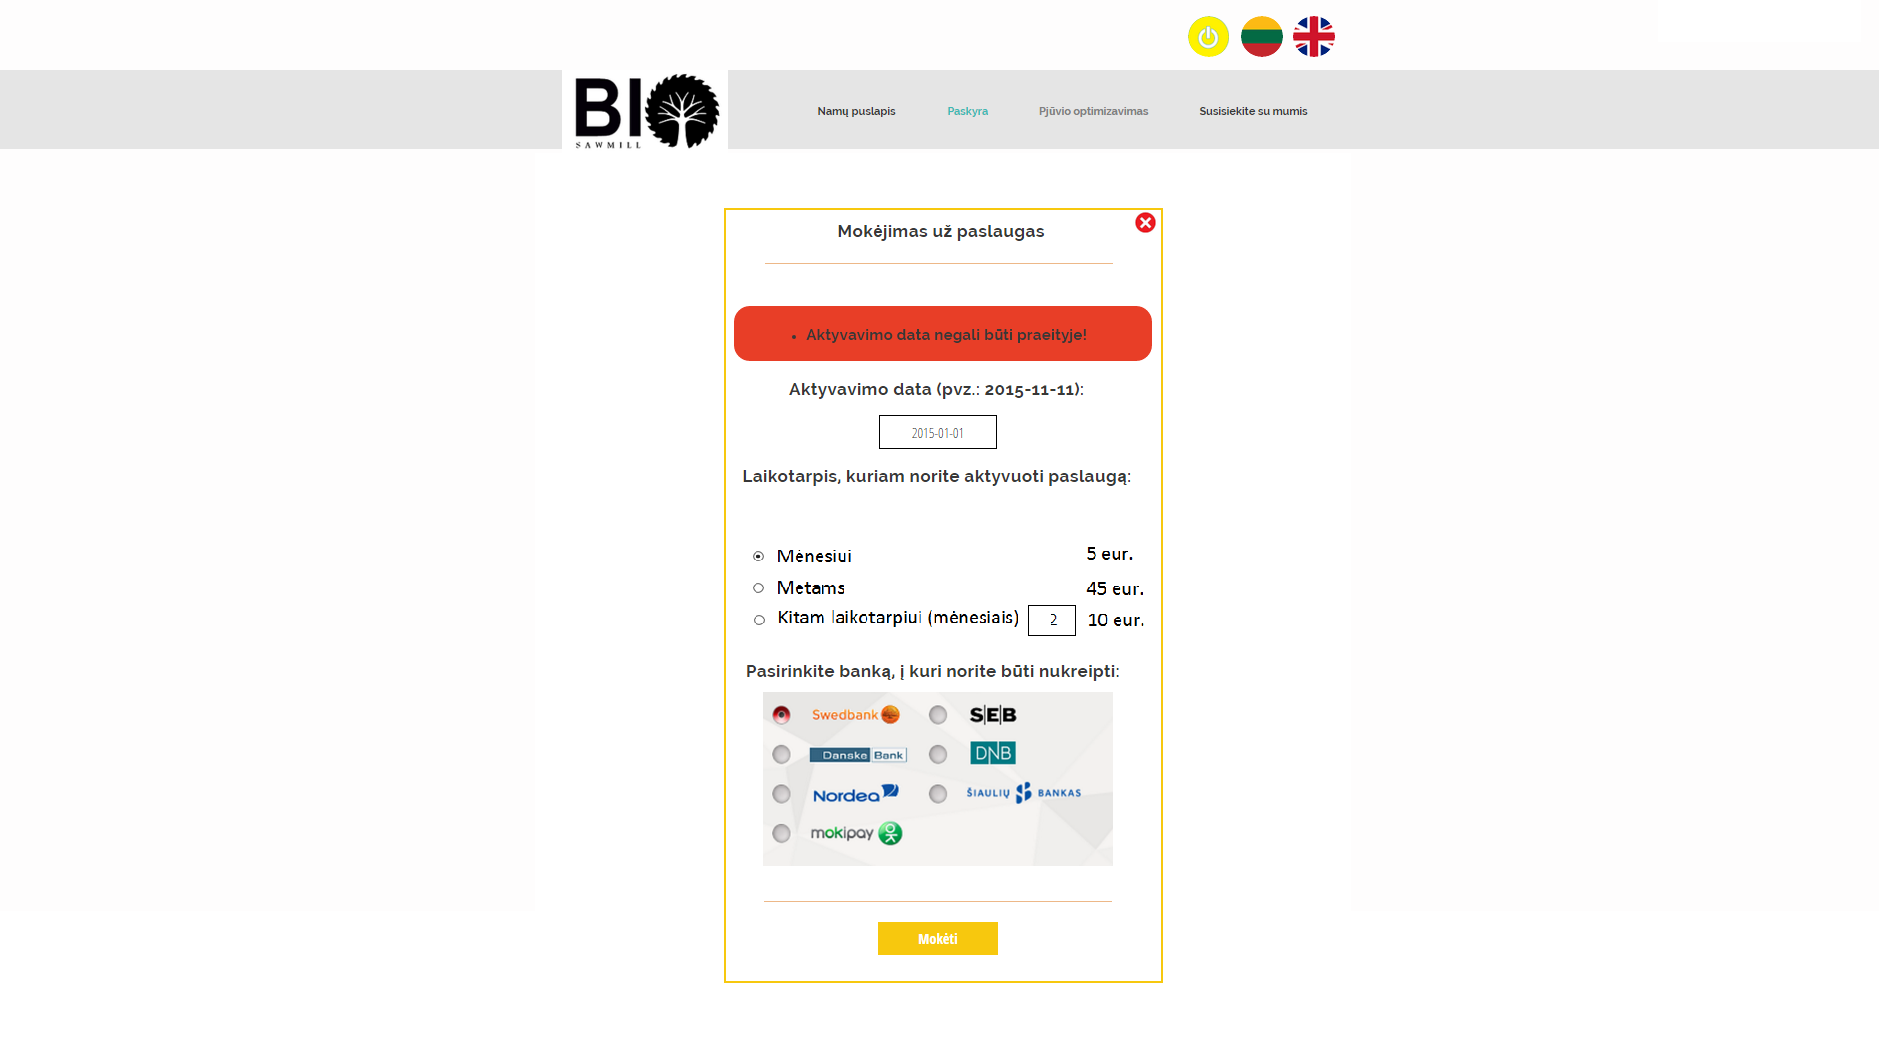
\includegraphics[scale=0.45]{interfeisai/paskyrosPuslapisVartotojasMokejimasSuKlaida}
\label{fig:verticalcell}
\end{figure}


\floatfoot{14 interfeisas. Vartotojo paskyros puslapis - administratorius}
\begin{figure}[!tph]
\hspace{-2cm}
\centering
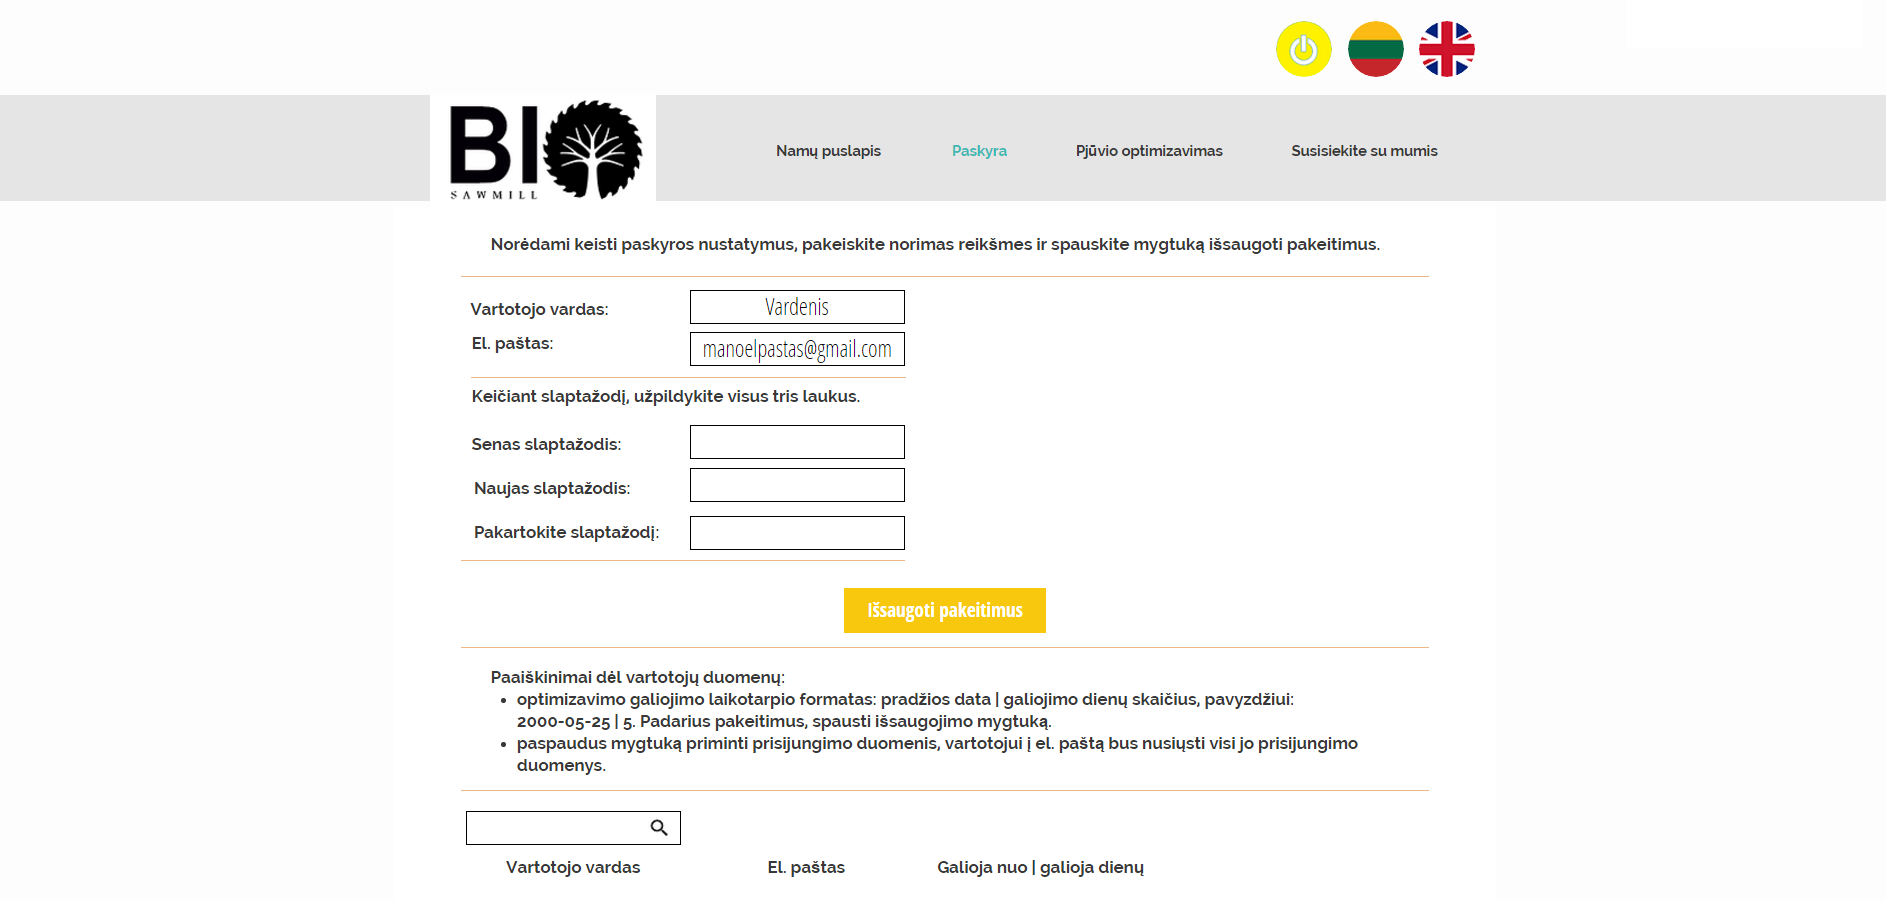
\includegraphics[scale=0.45]{interfeisai/paskyrosPuslapisAdministratorius}
\label{fig:verticalcell}
\end{figure}

\clearpage

\floatfoot{15 interfeisas. Vartotojo paskyros puslapis - administratorius (su klaida). "Floppy disc" išsaugo pakeitimus padarytus konkrečiai vartotojo paskyrai, o šiukšlinės ikona leidžia ištrinti vartotojo paskyrą prieš tai nukrepiant vartotoją į 15.1 dialogą.}
\begin{figure}[!tph]
\hspace{-2cm}
\centering
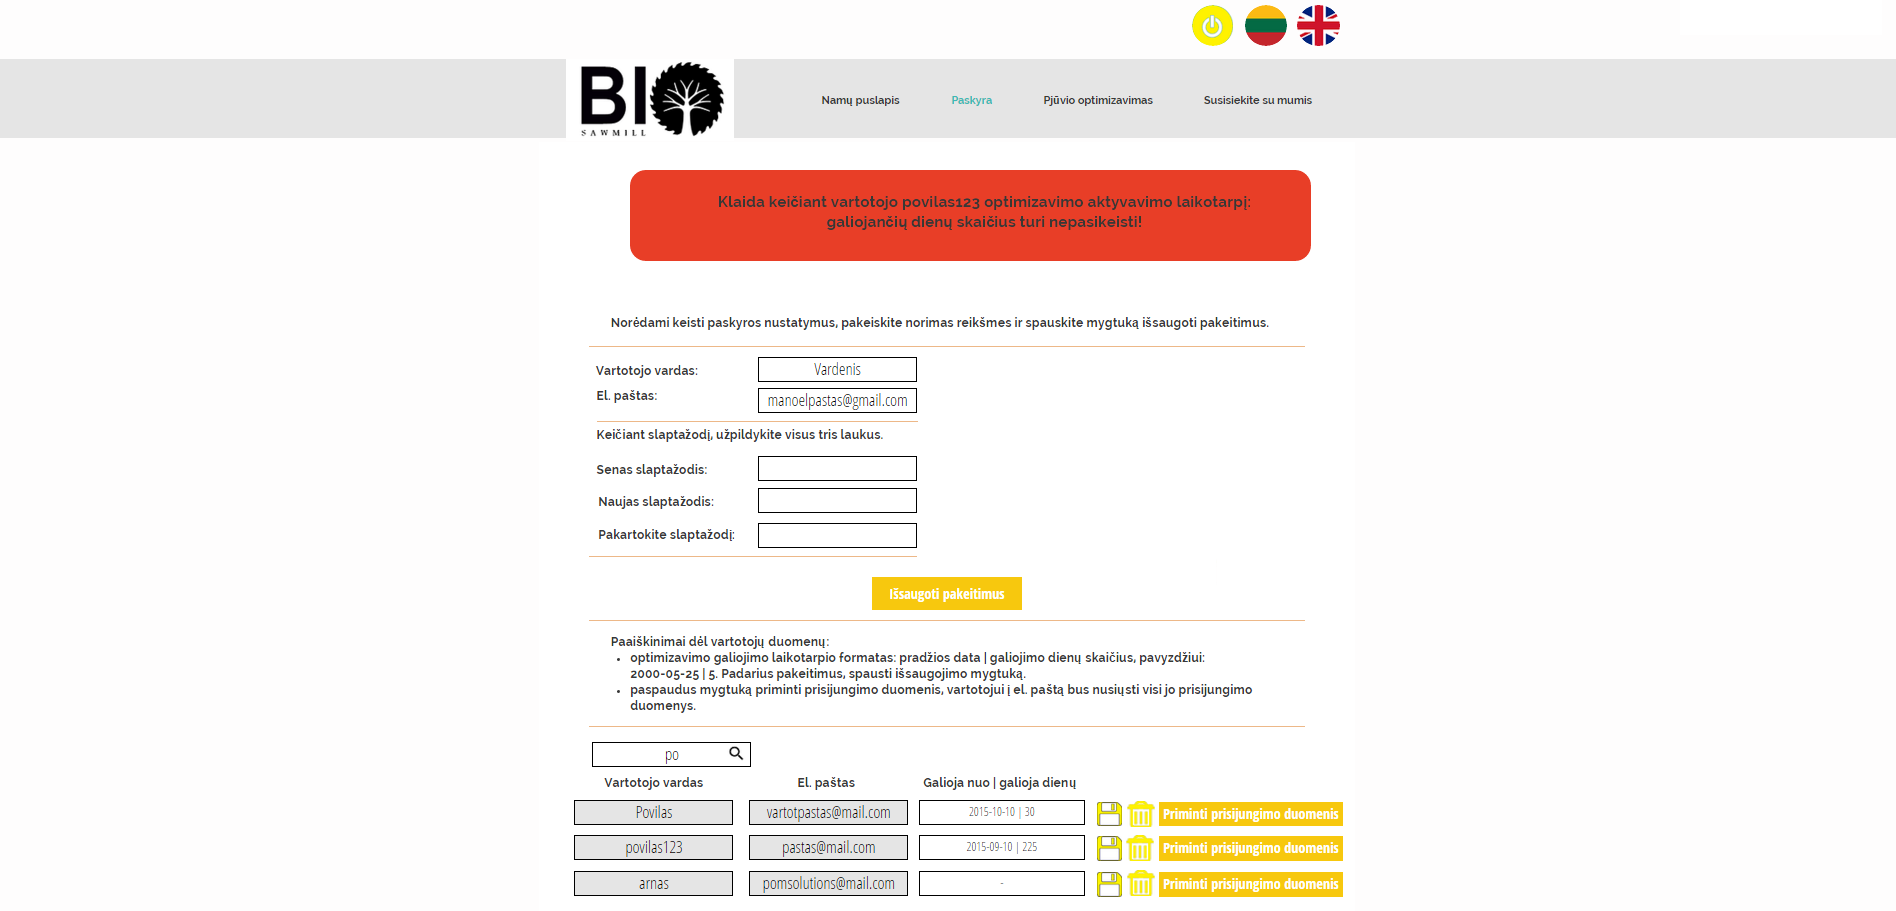
\includegraphics[scale=0.45]{interfeisai/paskyrosPuslapisAdministratoriusSuKlaida}
\label{fig:verticalcell}
\end{figure}

\floatfoot{15.1 interfeisas. Vartotojo paskyros puslapis - administratorius nori ištrinti vartotoją.}
\begin{figure}[!tph]
\hspace{-2cm}
\centering
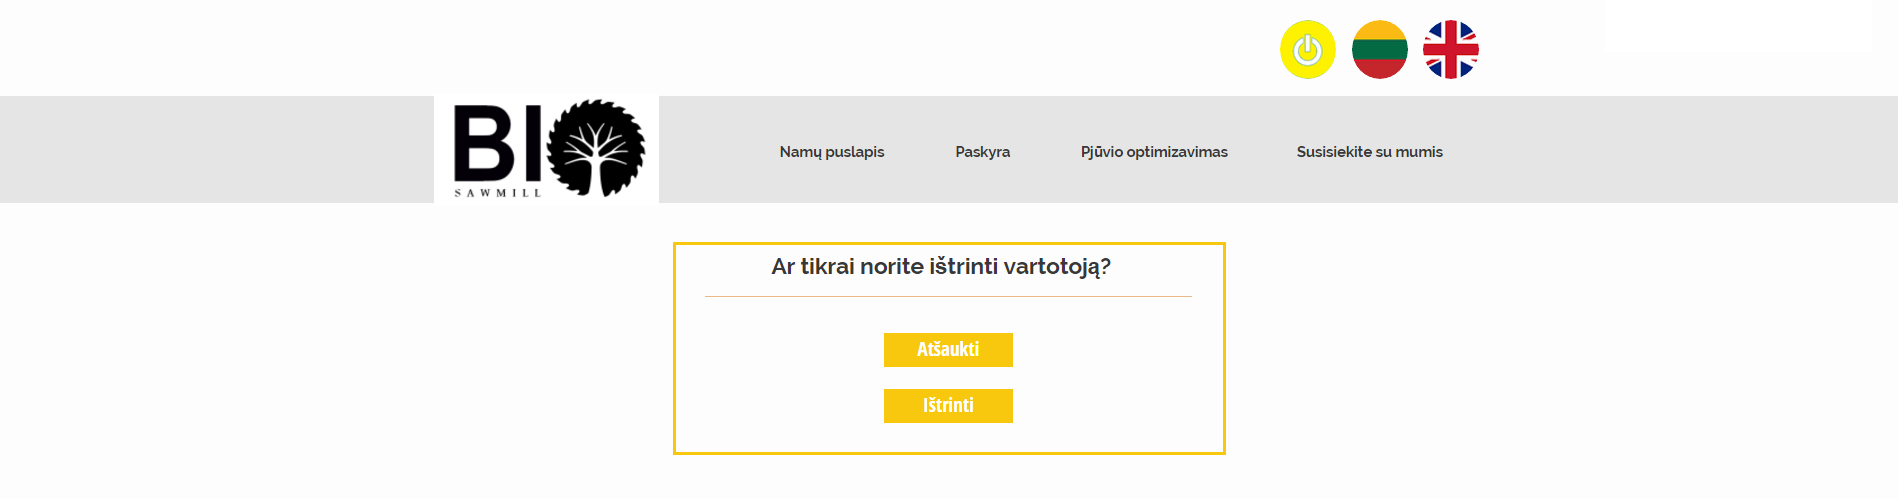
\includegraphics[scale=0.45]{interfeisai/vartotojoPaskyraVartotojoIstrynimoPatvirtinimas}
\label{fig:verticalcell}
\end{figure}



\clearpage

\subsection{Optimizavimo puslapis}
\floatfoot{16 interfeisas. Optimizavimo puslapis - neprisijungus}
\begin{figure}[!tph]
\hspace{-2cm}
\centering
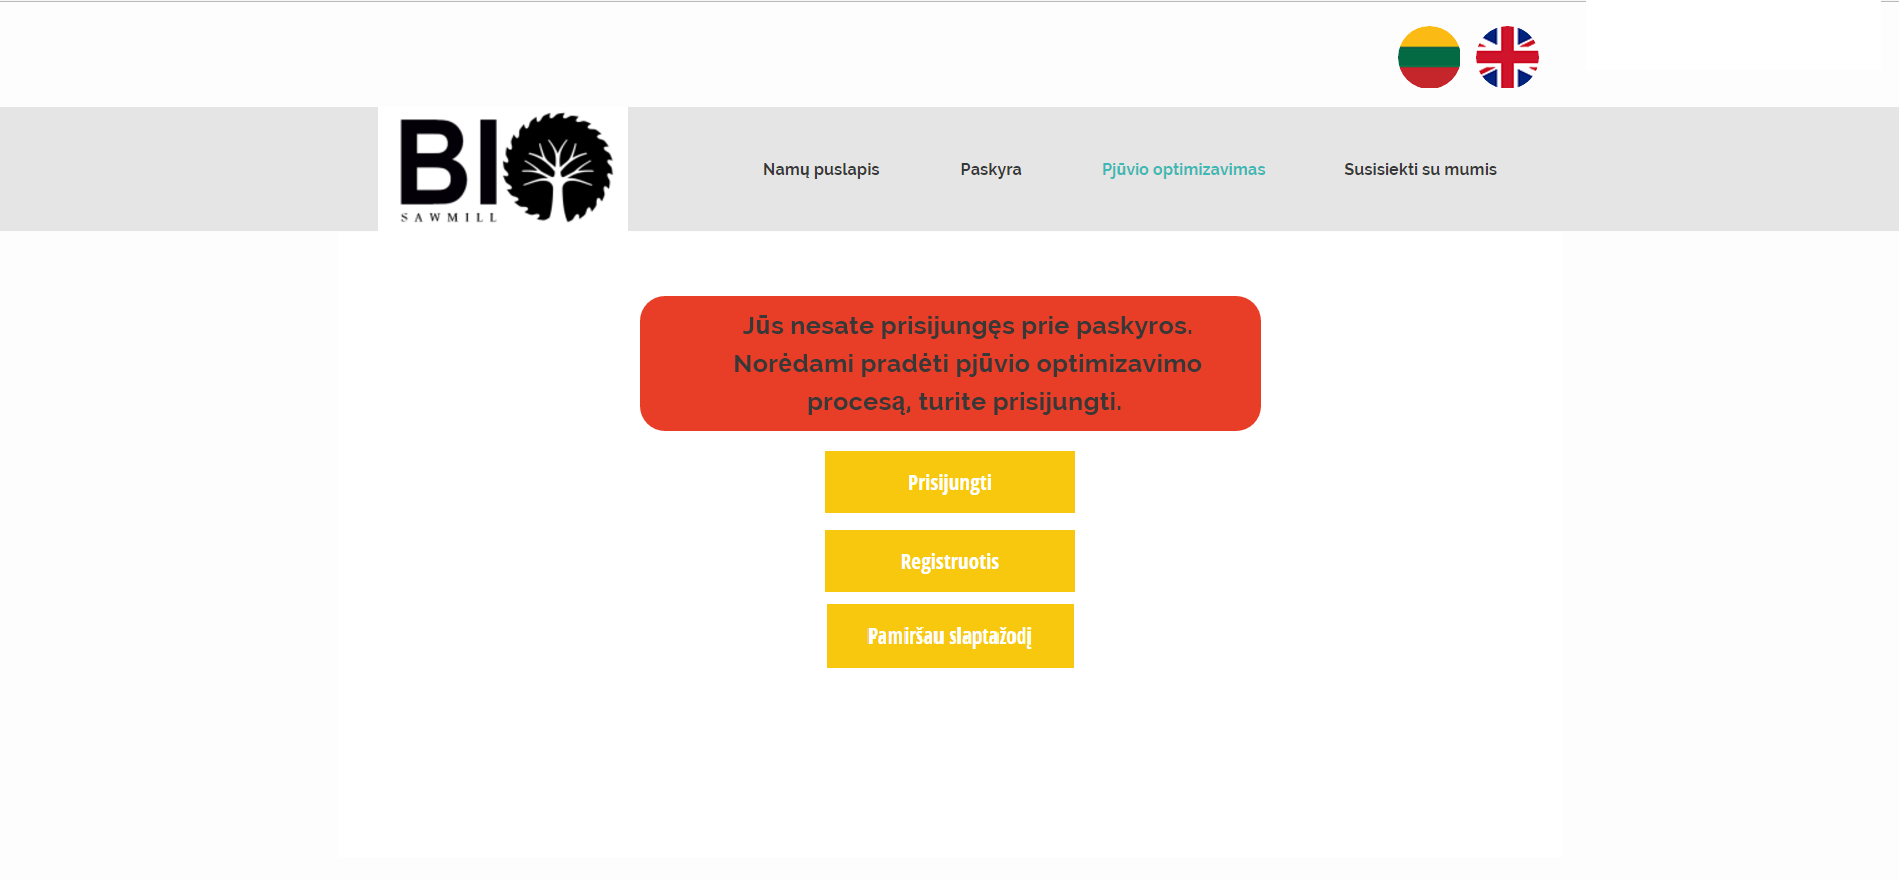
\includegraphics[scale=0.45]{interfeisai/optimizavimoPuslapisNeprisijungus}
\label{fig:verticalcell}
\end{figure}

\floatfoot{17 interfeisas. Optimizavimo puslapis - prisijungus. Vartotojui paspaudus "Pridėti naują" atsiradna nauji duomenų įvedimo laukeliai atitinkamai  prie detalių arbą panelių. "Importuoti iš failo (csv)" mygtukas atidary standartinį operacinės sistemos failo pasirinkimo langą. "Optimizuoti pjūvio planą" mygtukas atodaro 19 interfeisą (dialogą), o "Istorijos" mygtukas 23-ią interfeisą (dialogą).}
\begin{figure}[!tph]
\hspace{-2cm}
\centering
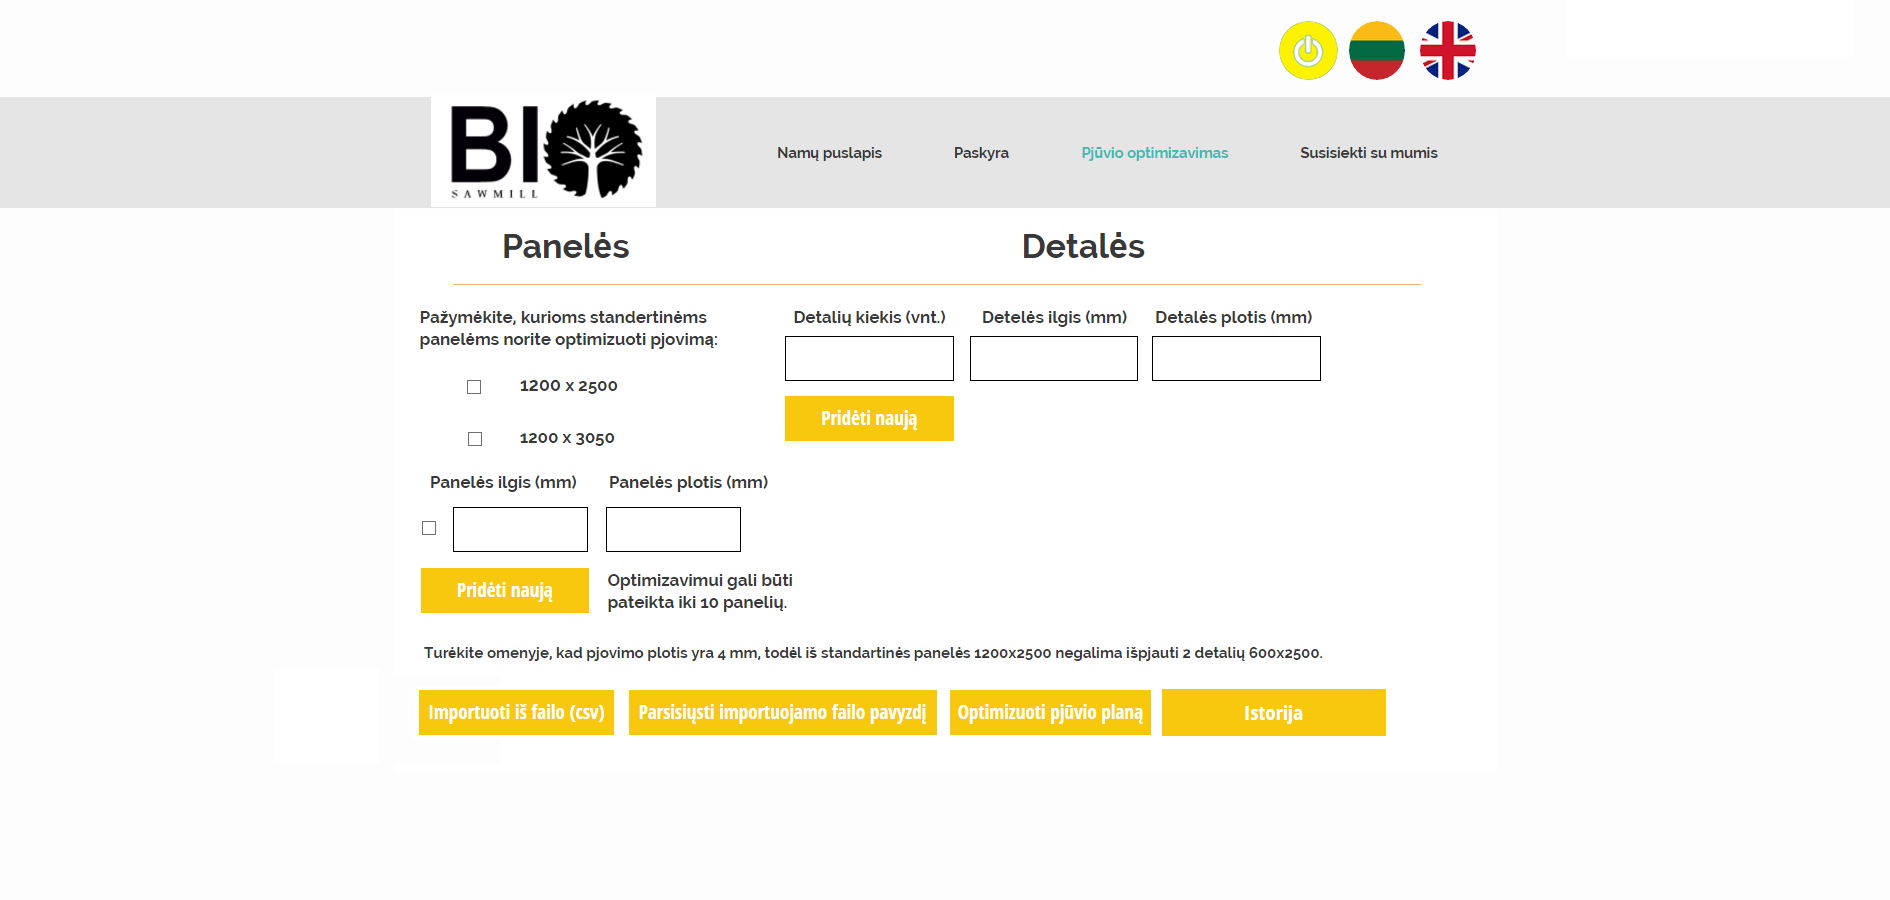
\includegraphics[scale=0.45]{interfeisai/optimizavimoPuslapisPrisijungus}
\label{fig:verticalcell}
\end{figure}

\floatfoot{18 interfeisas. Optimizavimo puslapis - prisijungus (su klaida)}
\begin{figure}[!tph]
\hspace{-2cm}
\centering
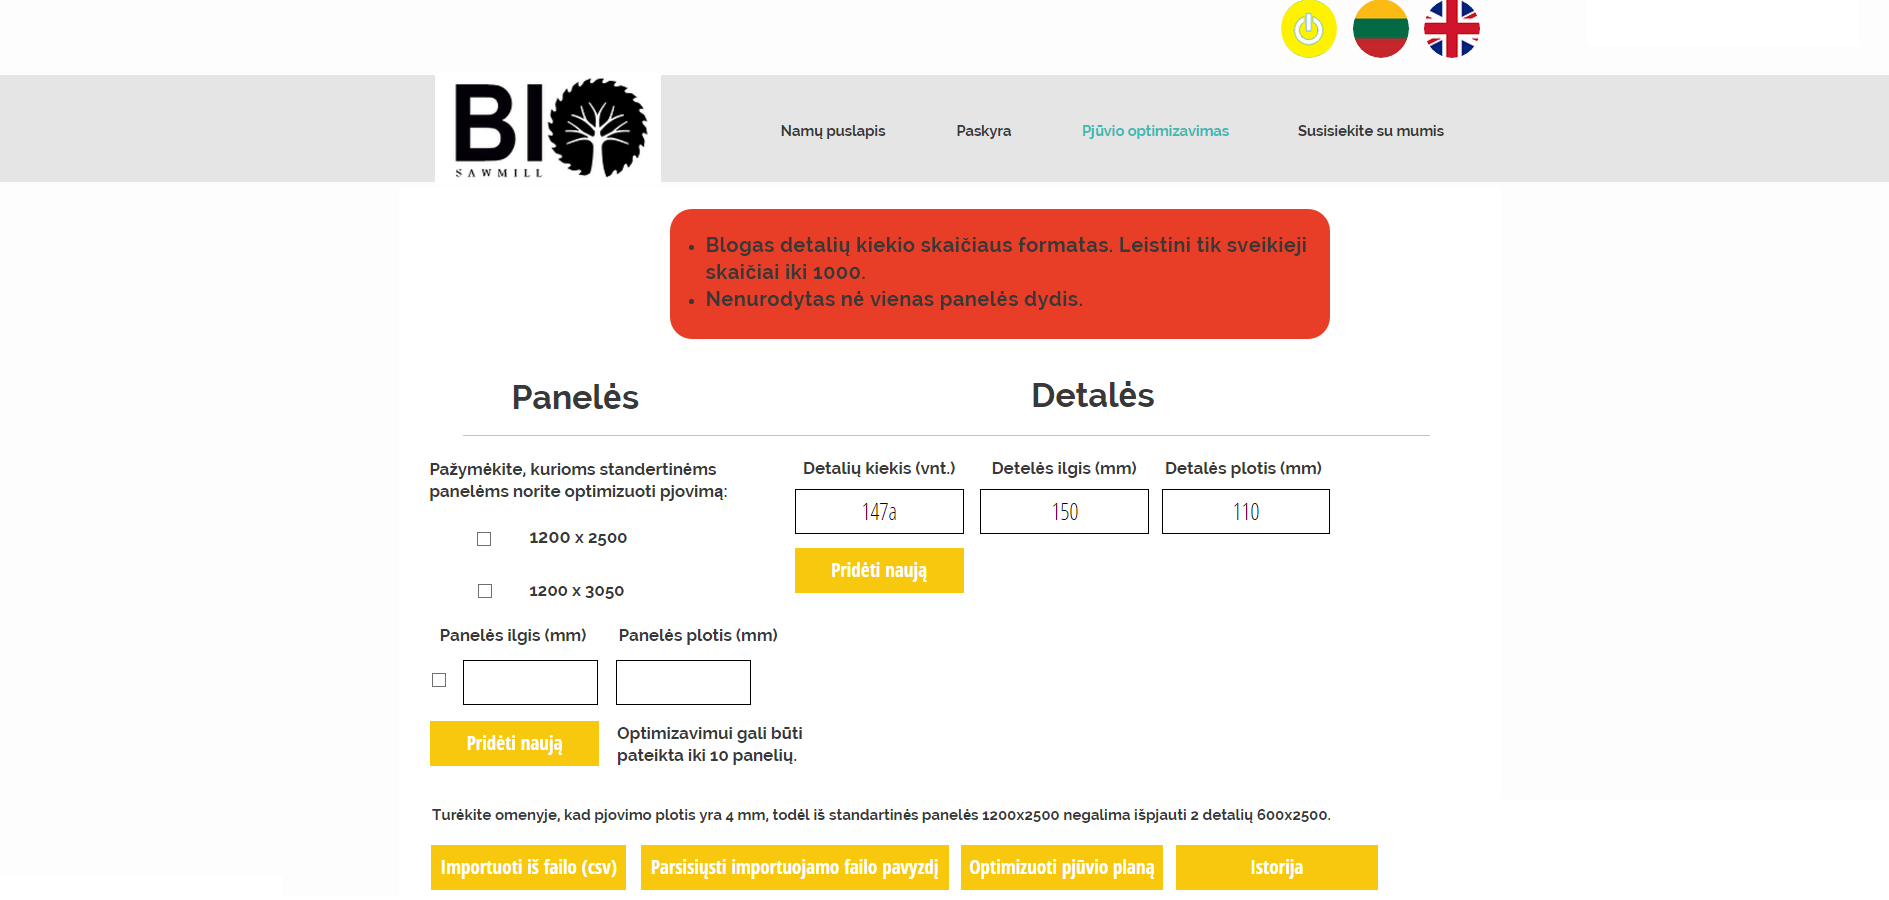
\includegraphics[scale=0.45]{interfeisai/optimizavimoPuslapisPrisijungusSuKlaida}
\label{fig:verticalcell}
\end{figure}


\floatfoot{19 interfeisas. Optimizavimo puslapis - po optimizavimo proceso. "Peržiūrėti planą" mygtukas atidaro 20 interfeisą (dialogą). Paspaudus "X" mygtuką visi optimizacijos gauti duomenys bus pamiršti.}
\begin{figure}[!tph]
\hspace{-2cm}
\centering
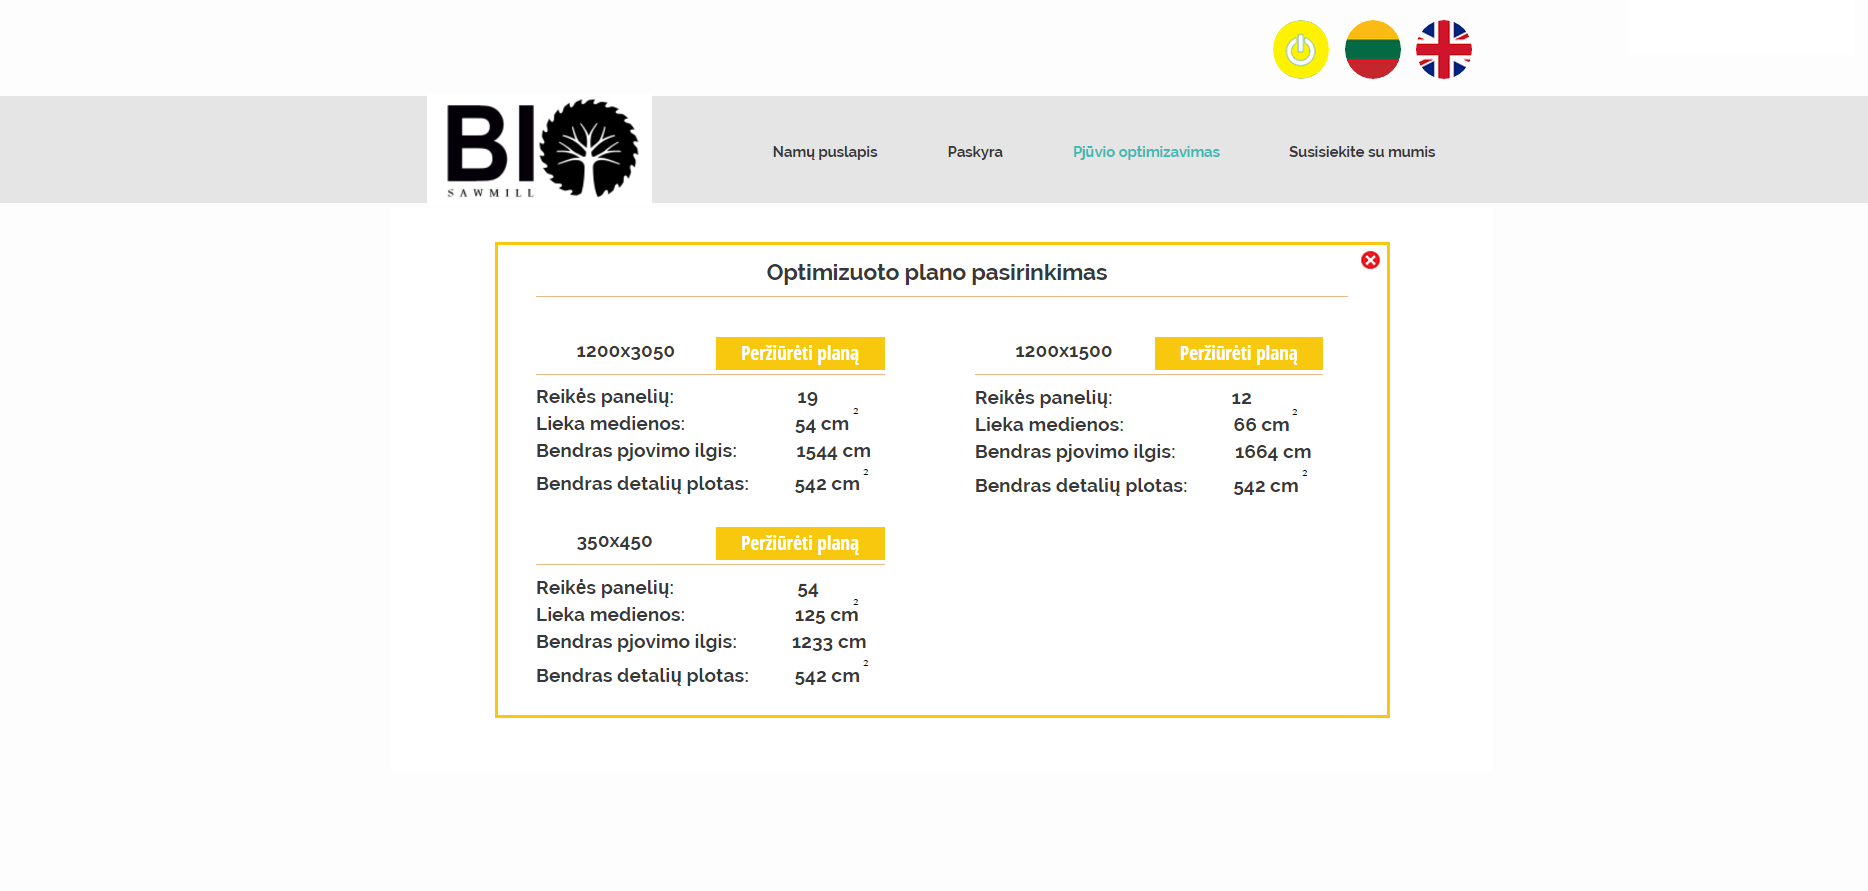
\includegraphics[scale=0.45]{interfeisai/optimizavimoPuslapisOptimizuotiPlanai}
\label{fig:verticalcell}
\end{figure}
\clearpage

\floatfoot{20 interfeisas. Optimizavimo puslapis - po optimizavimo, pasirinkus vieno iš planų peržiūrą (iš arčiau). Mygtukas "Parsisiųsti" atodaro standartinį operacinės sistemos failo išsaugojimo langą. Išsaugojimo mygtukas atodaro 21 interfeisą (dialogą), o  "Istorijos" mygtukas 23 interfeisą (dialogą).}
\begin{figure}[!tph]
\hspace{-2cm}
\centering
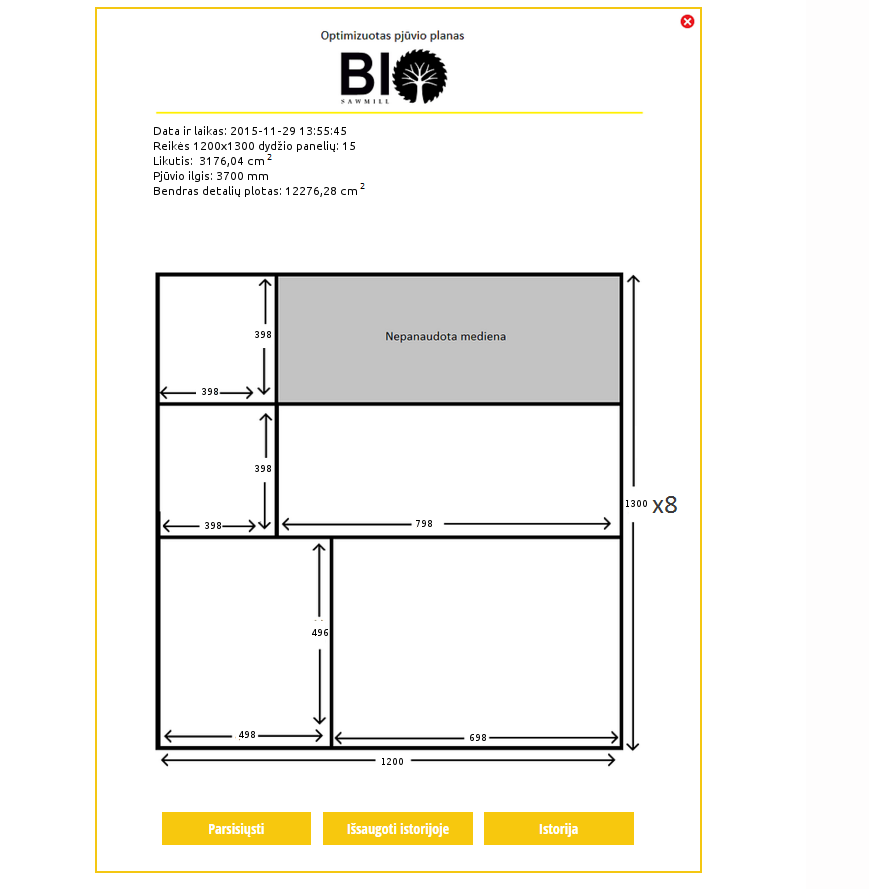
\includegraphics[scale=1]{interfeisai/optimizavimoPuslapisPrisijungusPasirinktoPerziura2}
\label{fig:horizontalcell}
\end{figure}


\floatfoot{21 interfeisas. Optimizavimo puslapis - pasirinkto plano išsaugojimas. Paspaudus mygtuką "Išsaugoti" šis dialogas yra uždaromas ir grįžtamą į 19 dialogą, tą patį atlieką ir "X" mygtukas.}
\begin{figure}[!tph]
\hspace{-2cm}
\centering
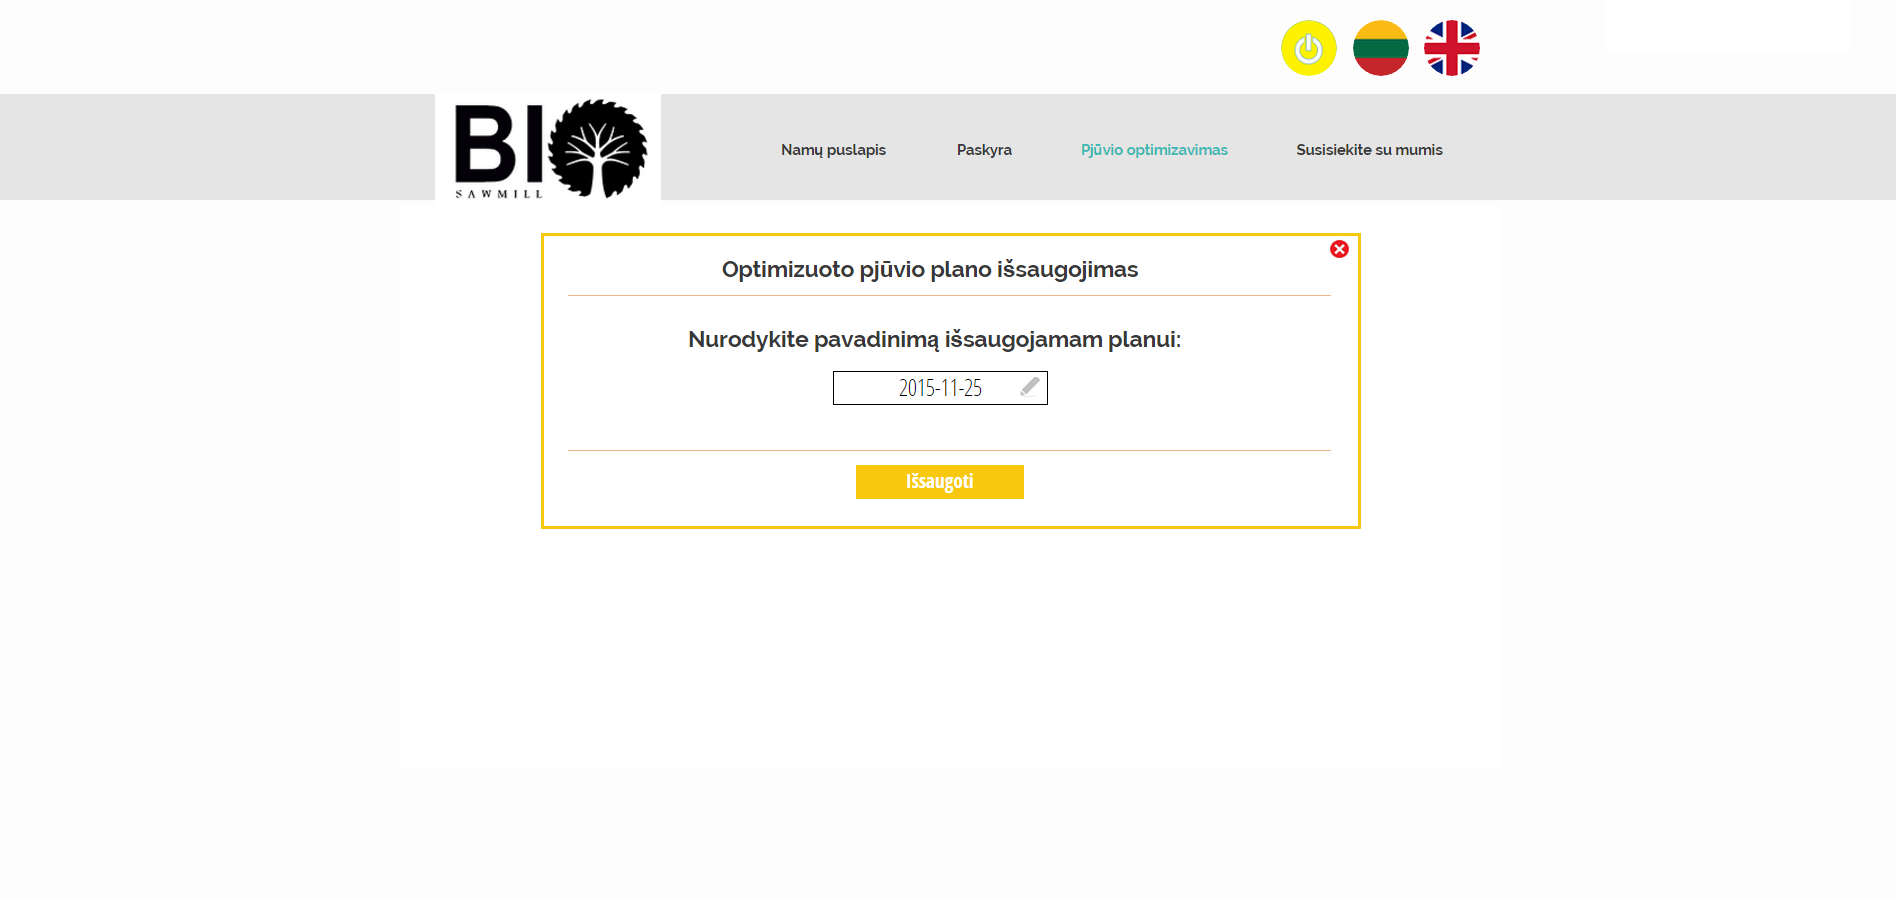
\includegraphics[scale=0.45]{interfeisai/optimizavimoPuslapisPrisijungusPasirinktoPlanoIsaugojimas}
\label{fig:verticalcell}
\end{figure}

\floatfoot{22 interfeisas. Optimizavimo puslapis - pasirinkto plano išsaugojimas (su klaida)}
\begin{figure}[!tph]
\hspace{-2cm}
\centering
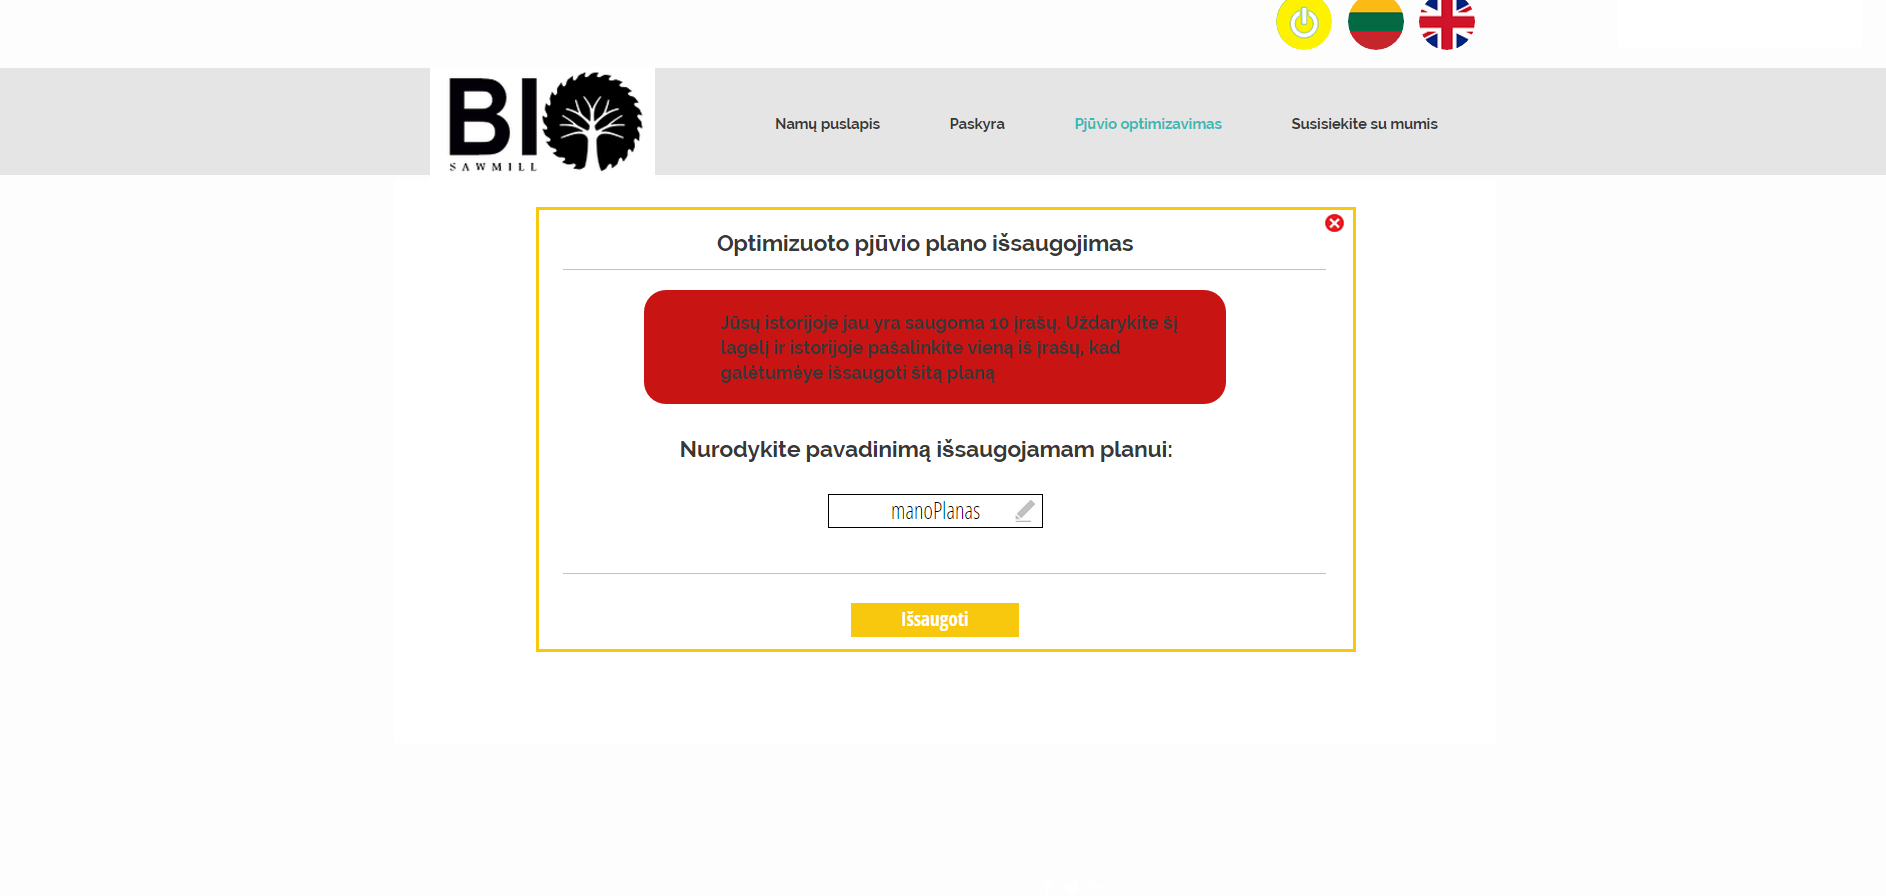
\includegraphics[scale=0.45]{interfeisai/optimizavimoPuslapisPrisijungusPasirinktoPlanoIsaugojimasSuKlaida}
\label{fig:verticalcell}
\end{figure}



\floatfoot{23 interfeisas. Optimizavimo puslapis - istorijos peržiūra. "Floppy disc" ikonos mygtukas išsaugo konkretaus įraši pakeitimus. Šiukšlinės ikona ištrina konkretų įrašą, o atsisiuntimo ikona atidaro standartinį operacinės sistemos duomenų išsaugojimo langą. "Peržiūrėti planą" mygtukas atidato 25 interfeisą (dialogą).}
\begin{figure}[!tph]
\hspace{-2cm}
\centering
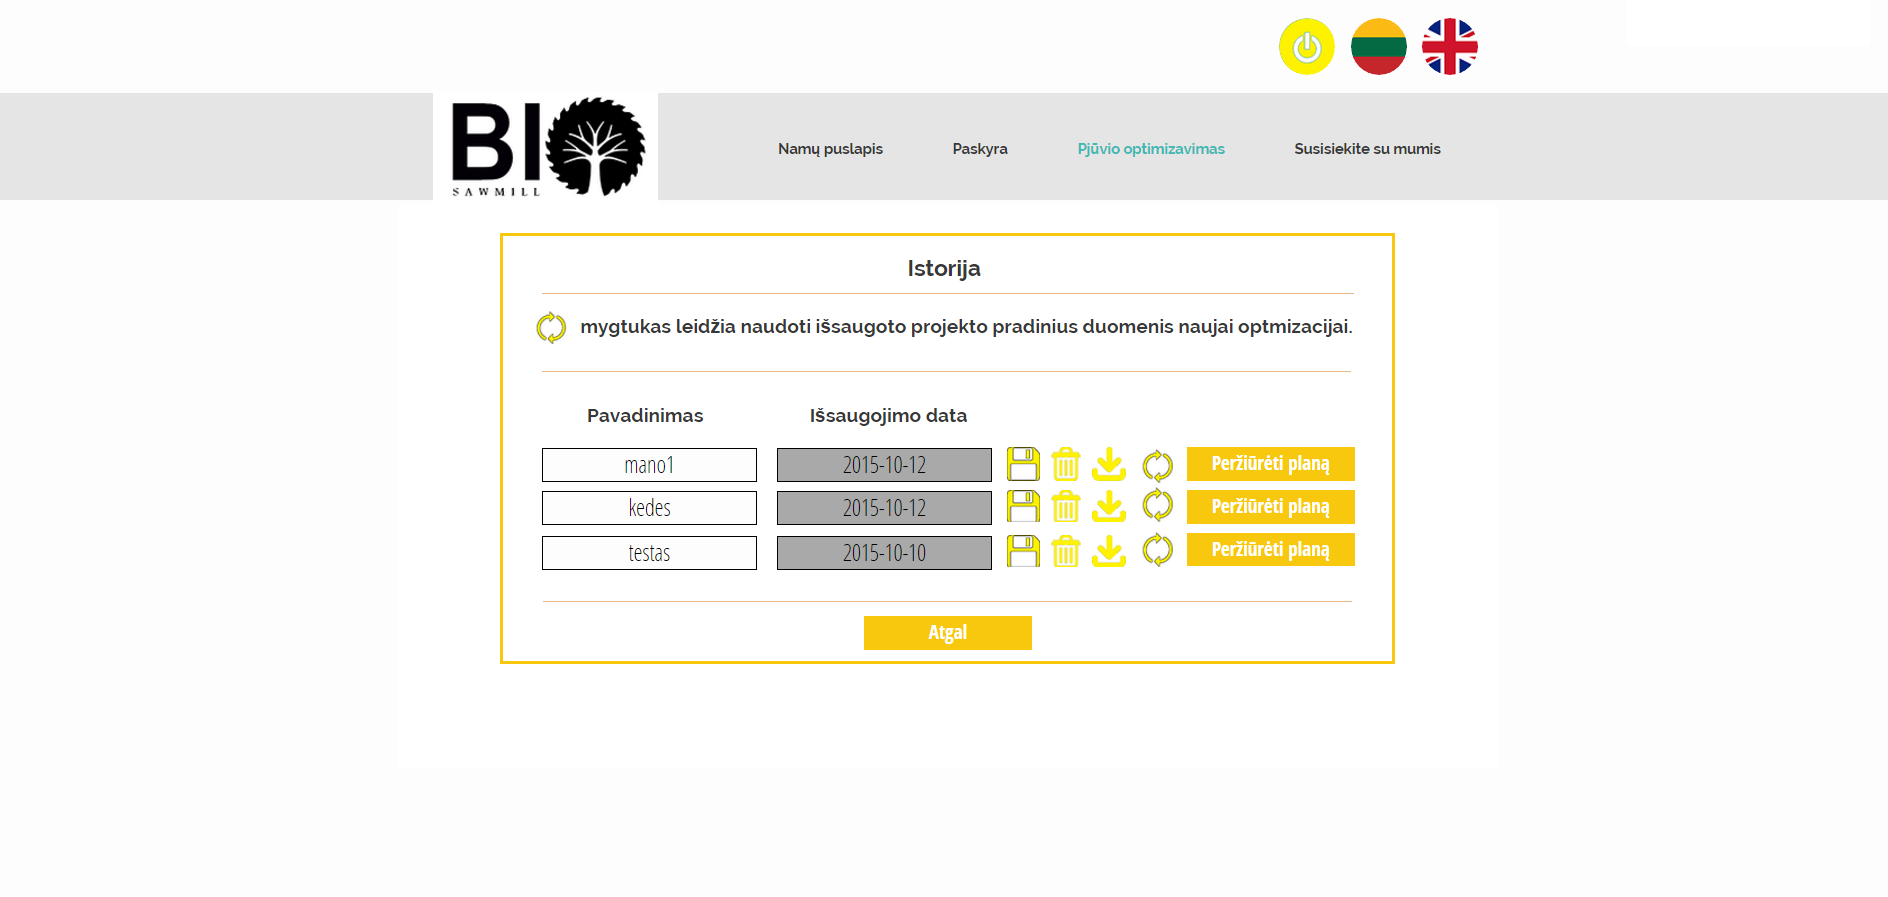
\includegraphics[scale=0.45]{interfeisai/optimizavimoPuslapisPrisijungusIstorija}
\label{fig:verticalcell}
\end{figure}


\floatfoot{24 interfeisas. Optimizavimo puslapis - istorijos redagavimas (su klaida)}
\begin{figure}[!tph]
\hspace{-2cm}
\centering
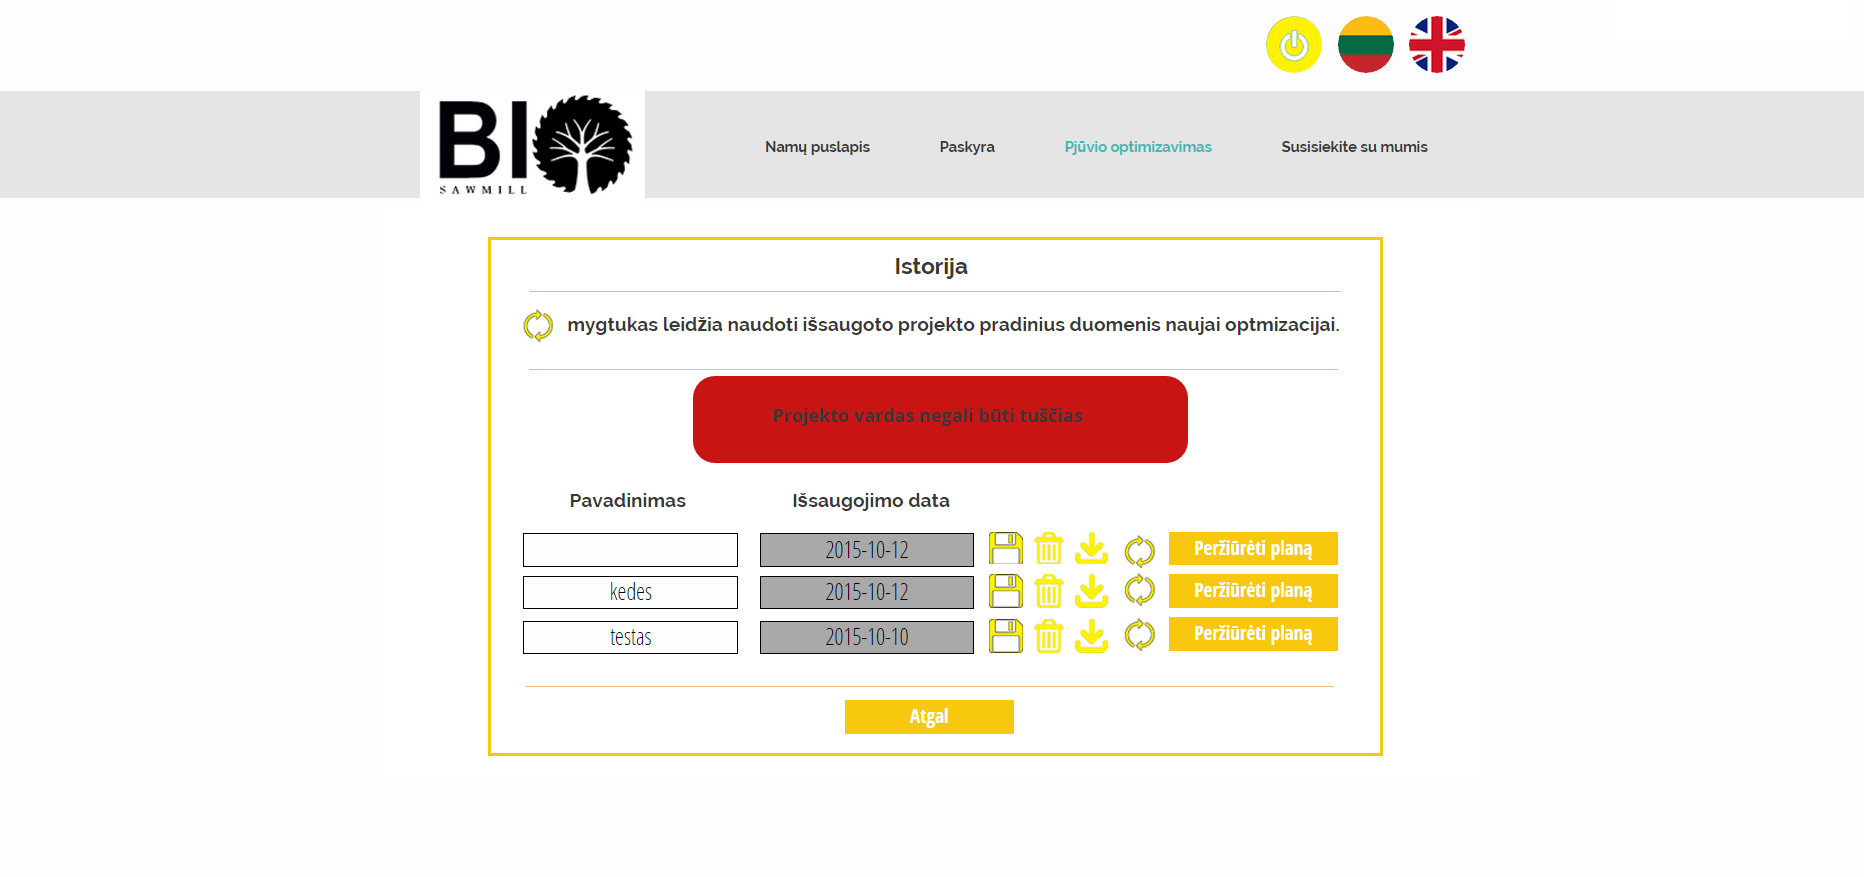
\includegraphics[scale=0.45]{interfeisai/optimizavimoPuslapisPrisijungusIstorijaSuKlaida}
\label{fig:verticalcell}
\end{figure}

\clearpage


\floatfoot{25 interfeisas. Optimizavimo puslapis - išsaugoto plano istorijoje peržiūra (iš arčiau). "X" mygtukas gražina vartotoją į 23 dialogą, o parsisiuntimo - atidaro standartinį operacinės sistemos failo išsaugojimo langą. Lange matomas "x8" nurodo kokiam kiekiui planlių reikės taikyti vaizduojamą pjųvio planą. Plano apačioje esančios dvi ikonos (geltona ir juoda) leidžia perjungti pjūvio plano vaizdą likusiam panelių kiekui. Vartotojo atsisiųstame pjūvio ruošinyje (pagal šį pavyzdį) vartotojas matytų šious du skirtingus planus einančius vienas po kito.} 
\begin{figure}[!tph]
\hspace{-2cm}
\centering
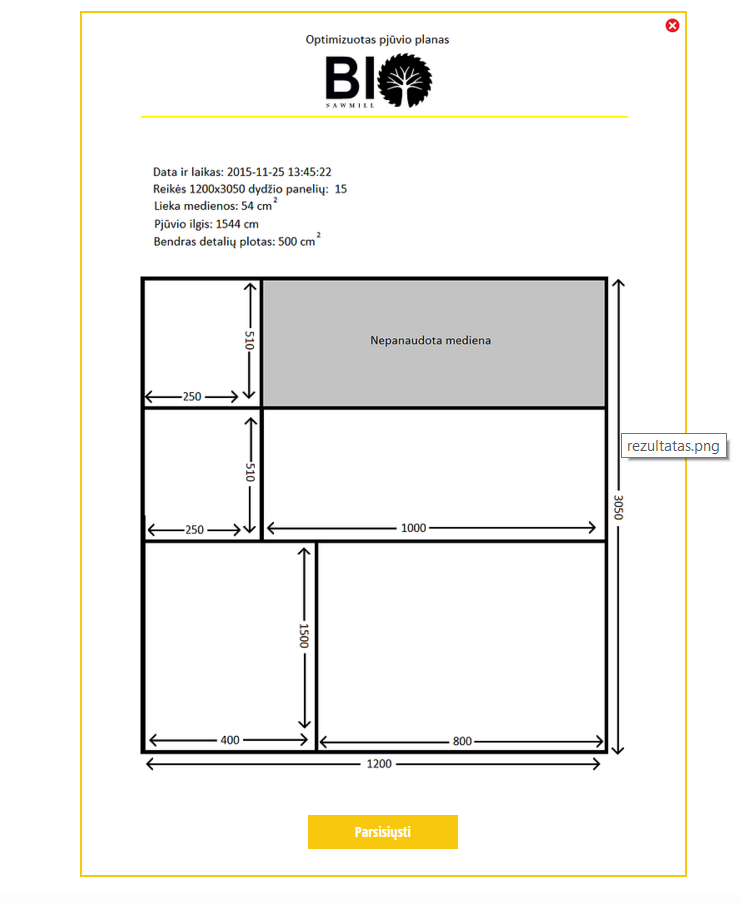
\includegraphics[scale=1]{interfeisai/optimizavimoPuslapisPrisijungusIsaugotasPlanas}
\label{fig:verticalcell}
\end{figure}

\clearpage

\subsection{Susisiekimo su mumis puslapis}


\floatfoot{26 interfeisas. Susisiekimo su mumis puslapis}
\begin{figure}[!tph]
\hspace{-2cm}
\centering
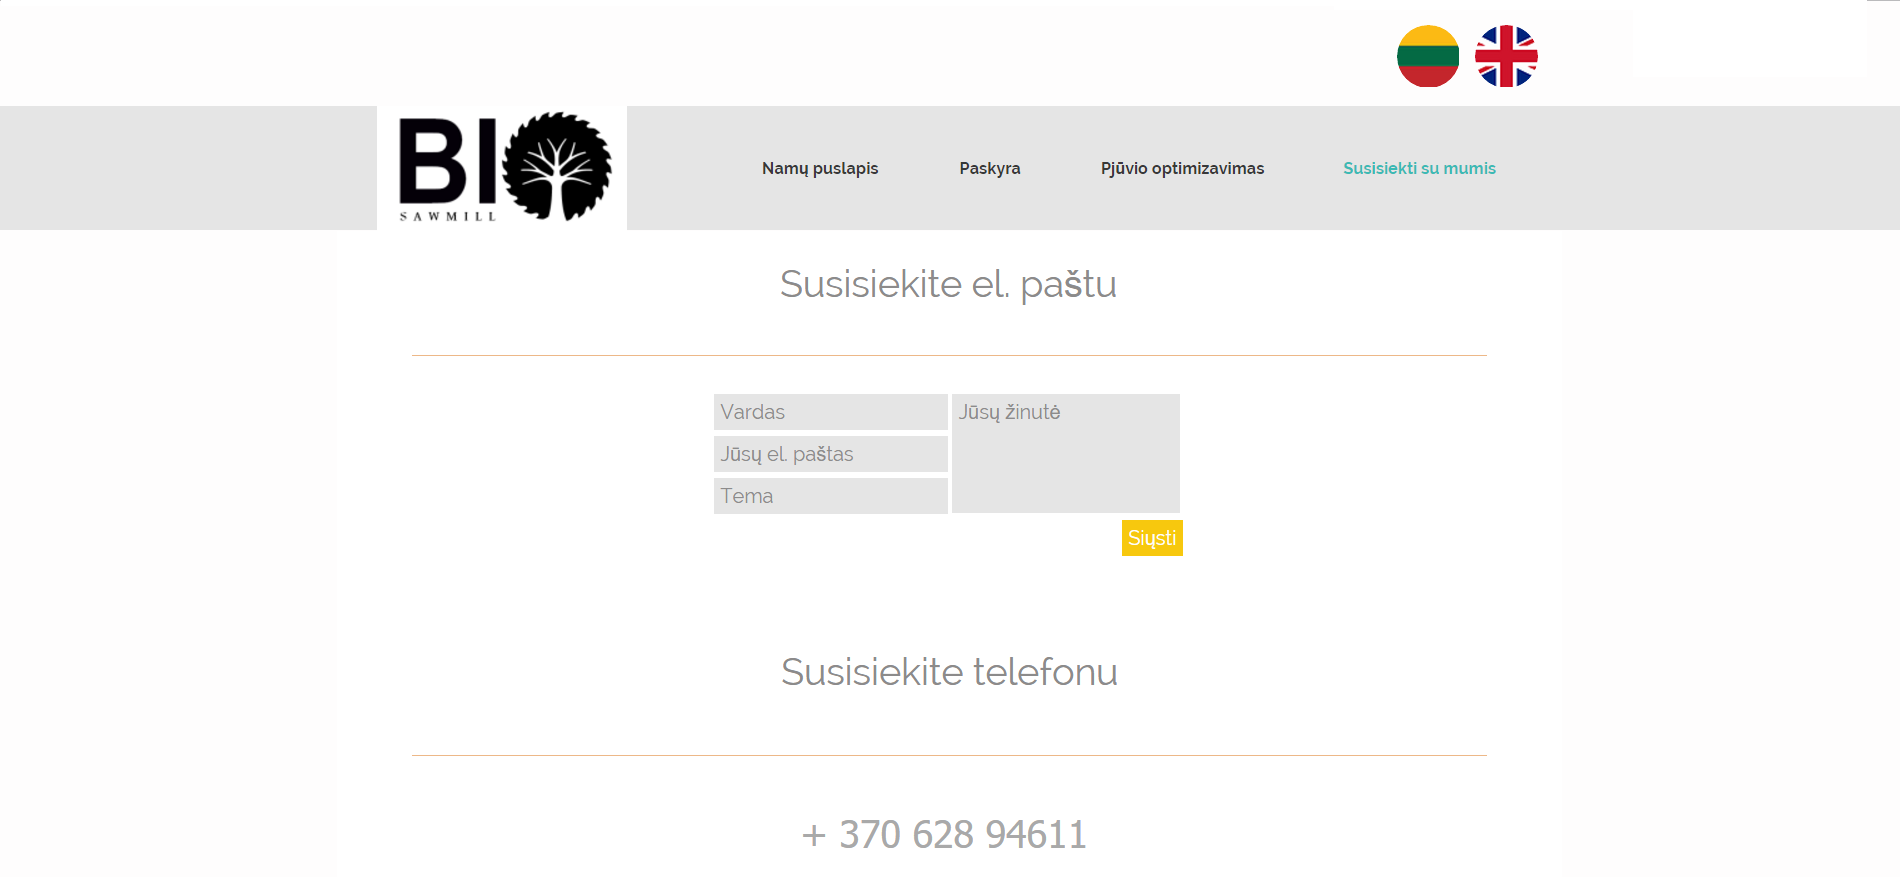
\includegraphics[scale=0.45]{interfeisai/susisiekimas}
\label{fig:verticalcell}
\end{figure}

\floatfoot{27 interfeisas. Susisiekimo su mumis puslapis (su klaida)}
\begin{figure}[!tph]
\hspace{-2cm}
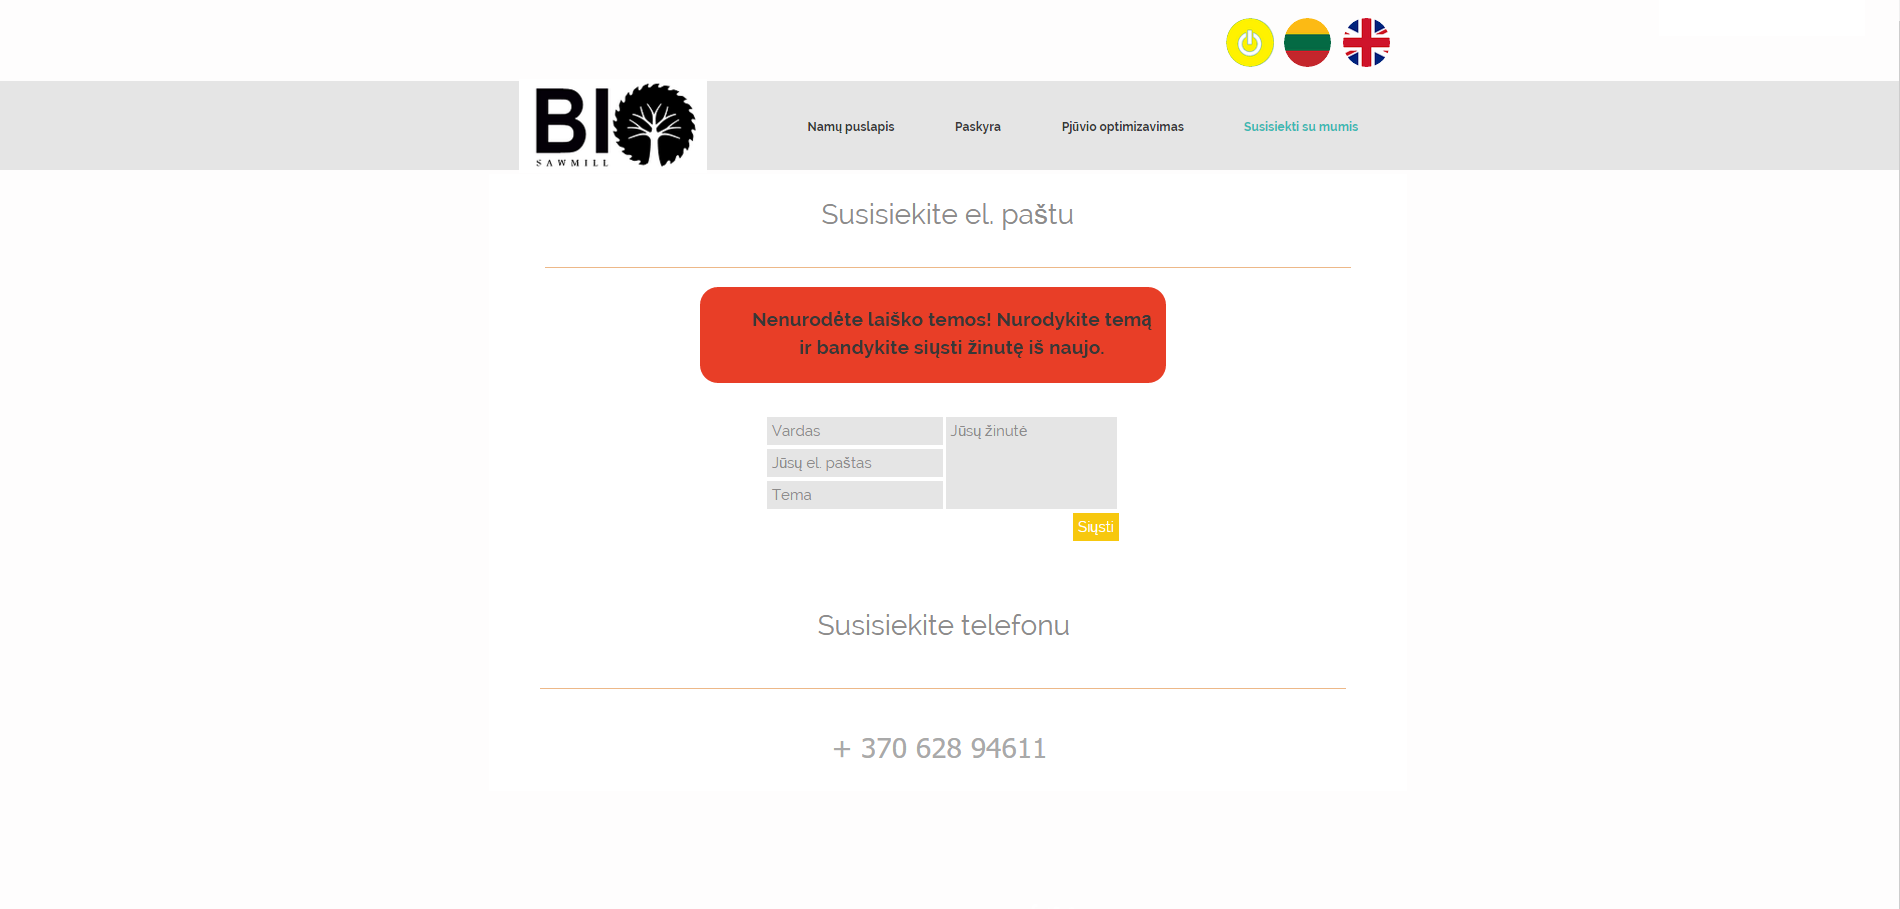
\includegraphics[scale=0.45]{interfeisai/susisiekimasSuKlaida}
\label{fig:verticalcell}
\end{figure}

\subsection{ Nenumatytos klaidos atvejis}
\floatfoot{28 interfeisas. Nenumatyta klaida}
\begin{figure}[!tph]
\hspace{-2cm}
\centering
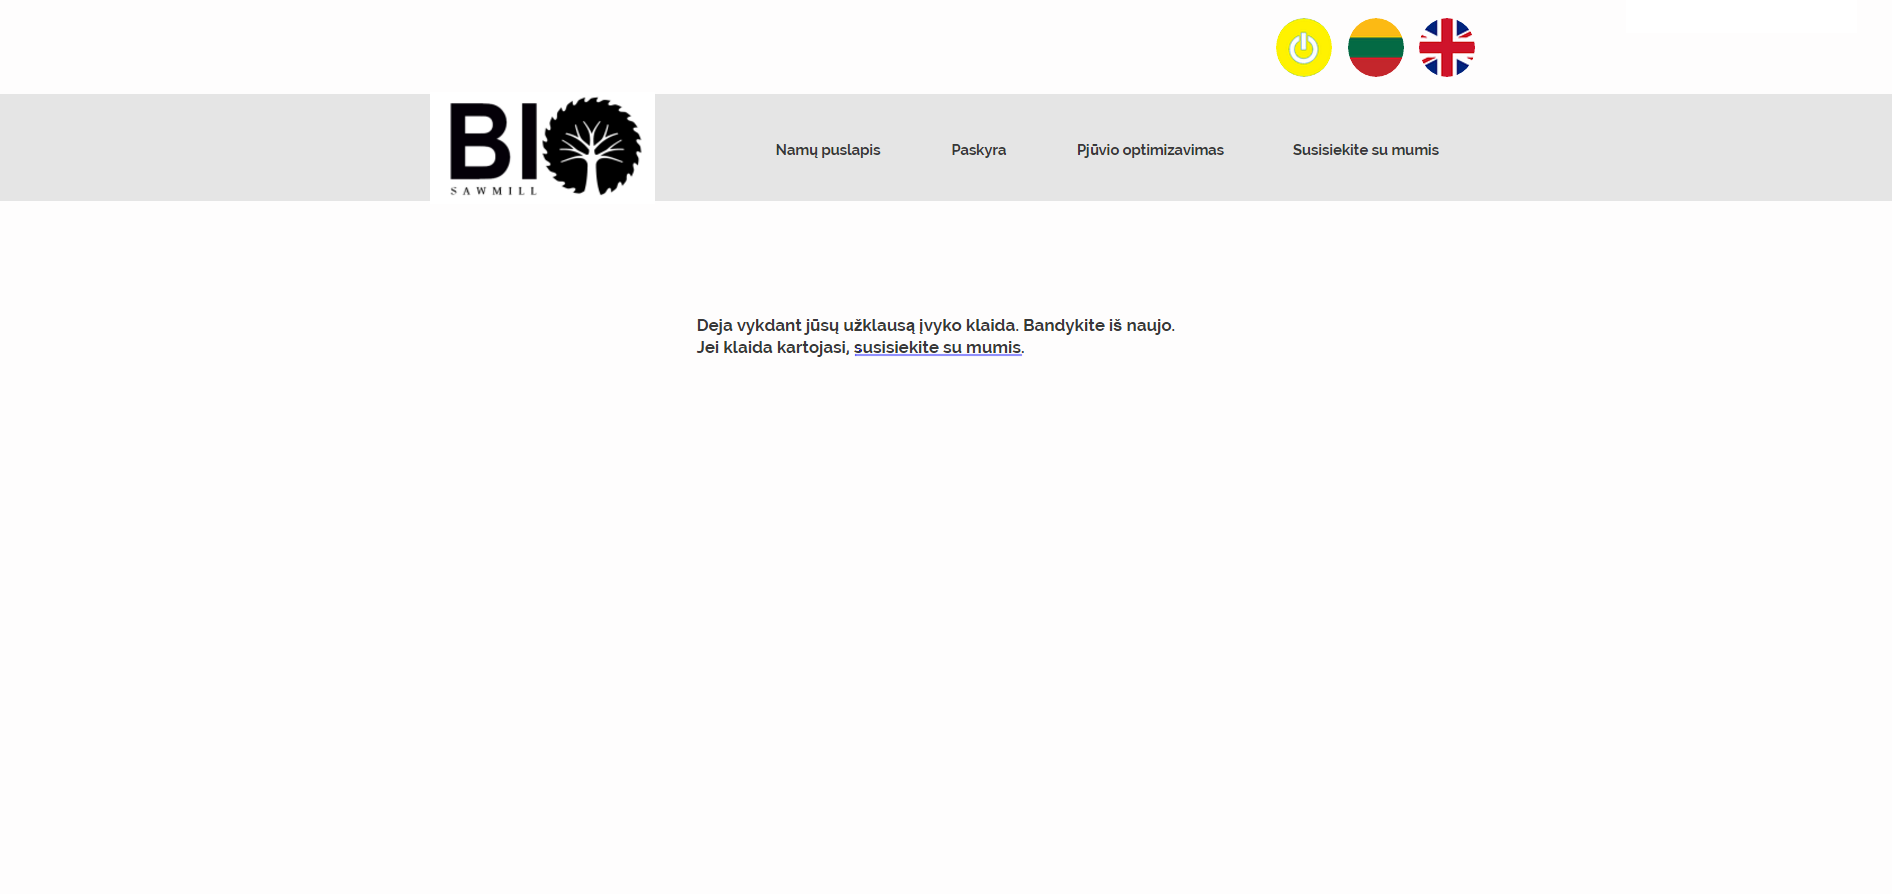
\includegraphics[scale=0.45]{interfeisai/bendraKlaida}
\label{fig:verticalcell}
\end{figure}

\clearpage

% ---------------------------------- UZKOMENTUOTA, NEISTRINTI  ------------------------------
\begin{comment}
\subsection{Namų puslapis (vartotojas prisijungęs)}
\subsection{Namų puslapis}


\hspace{-2cm}
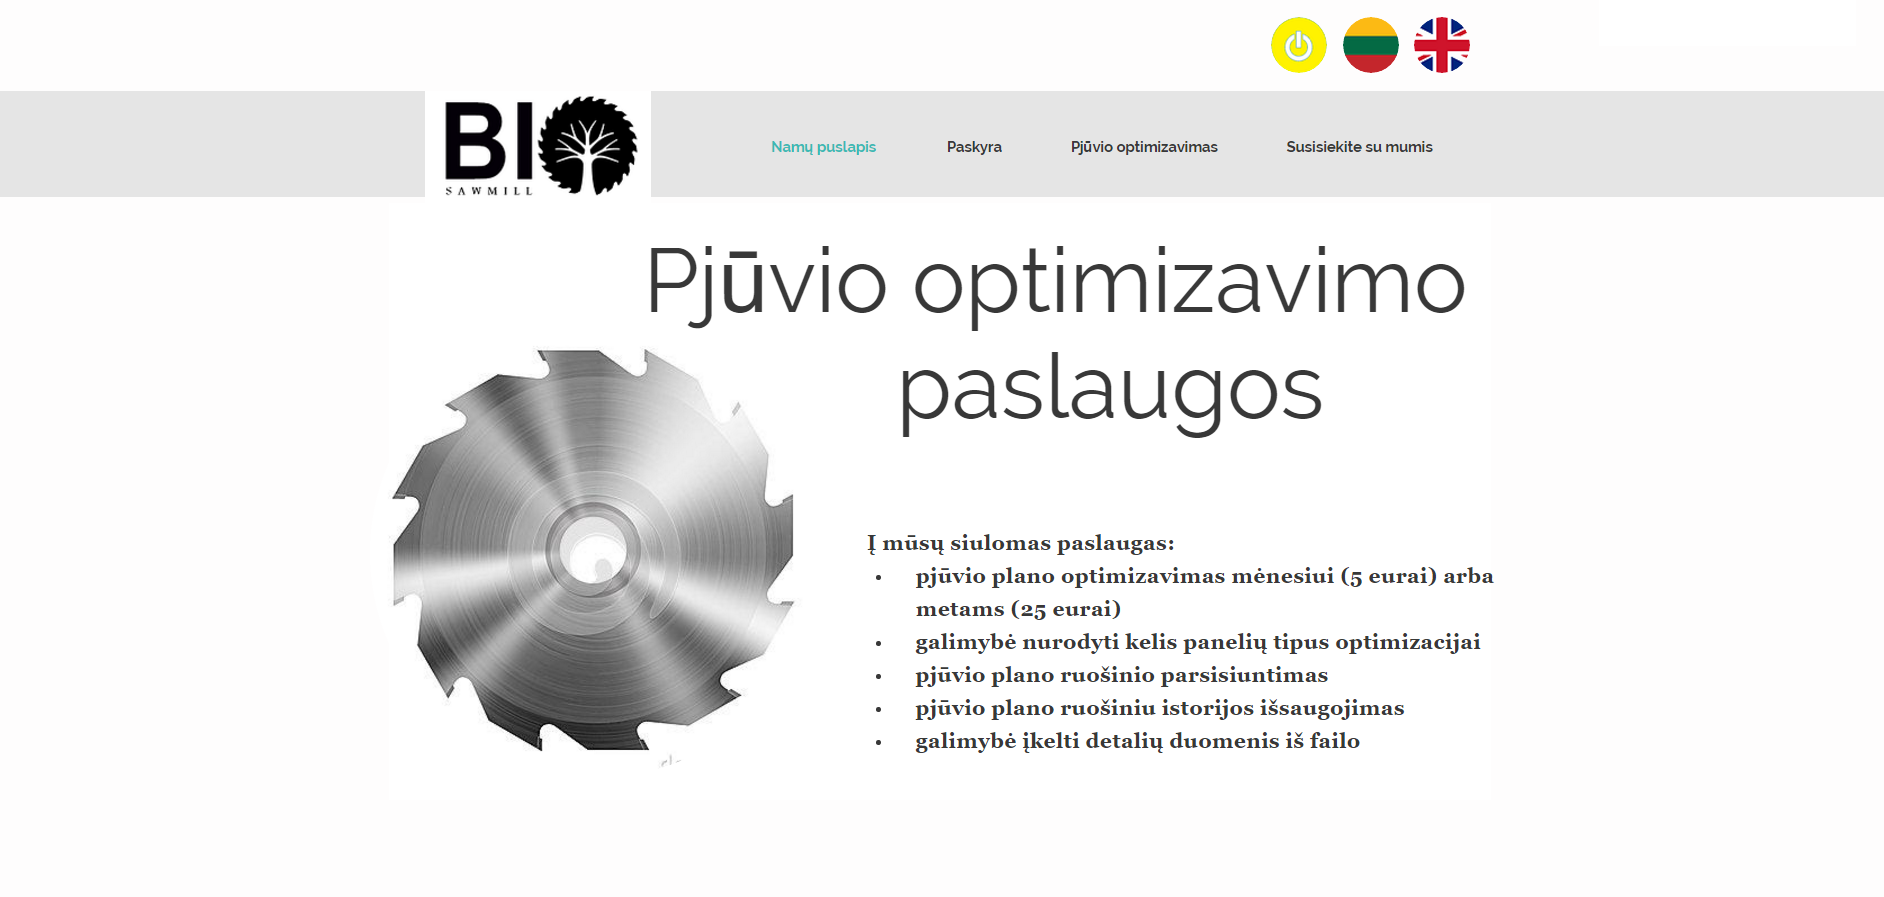
\includegraphics[scale=0.5]{interfeisai/pagrindinis}

\subsection{Vartotojo paskyros puslapis - vartotojas neprisijungęs}
\hspace{-2cm}
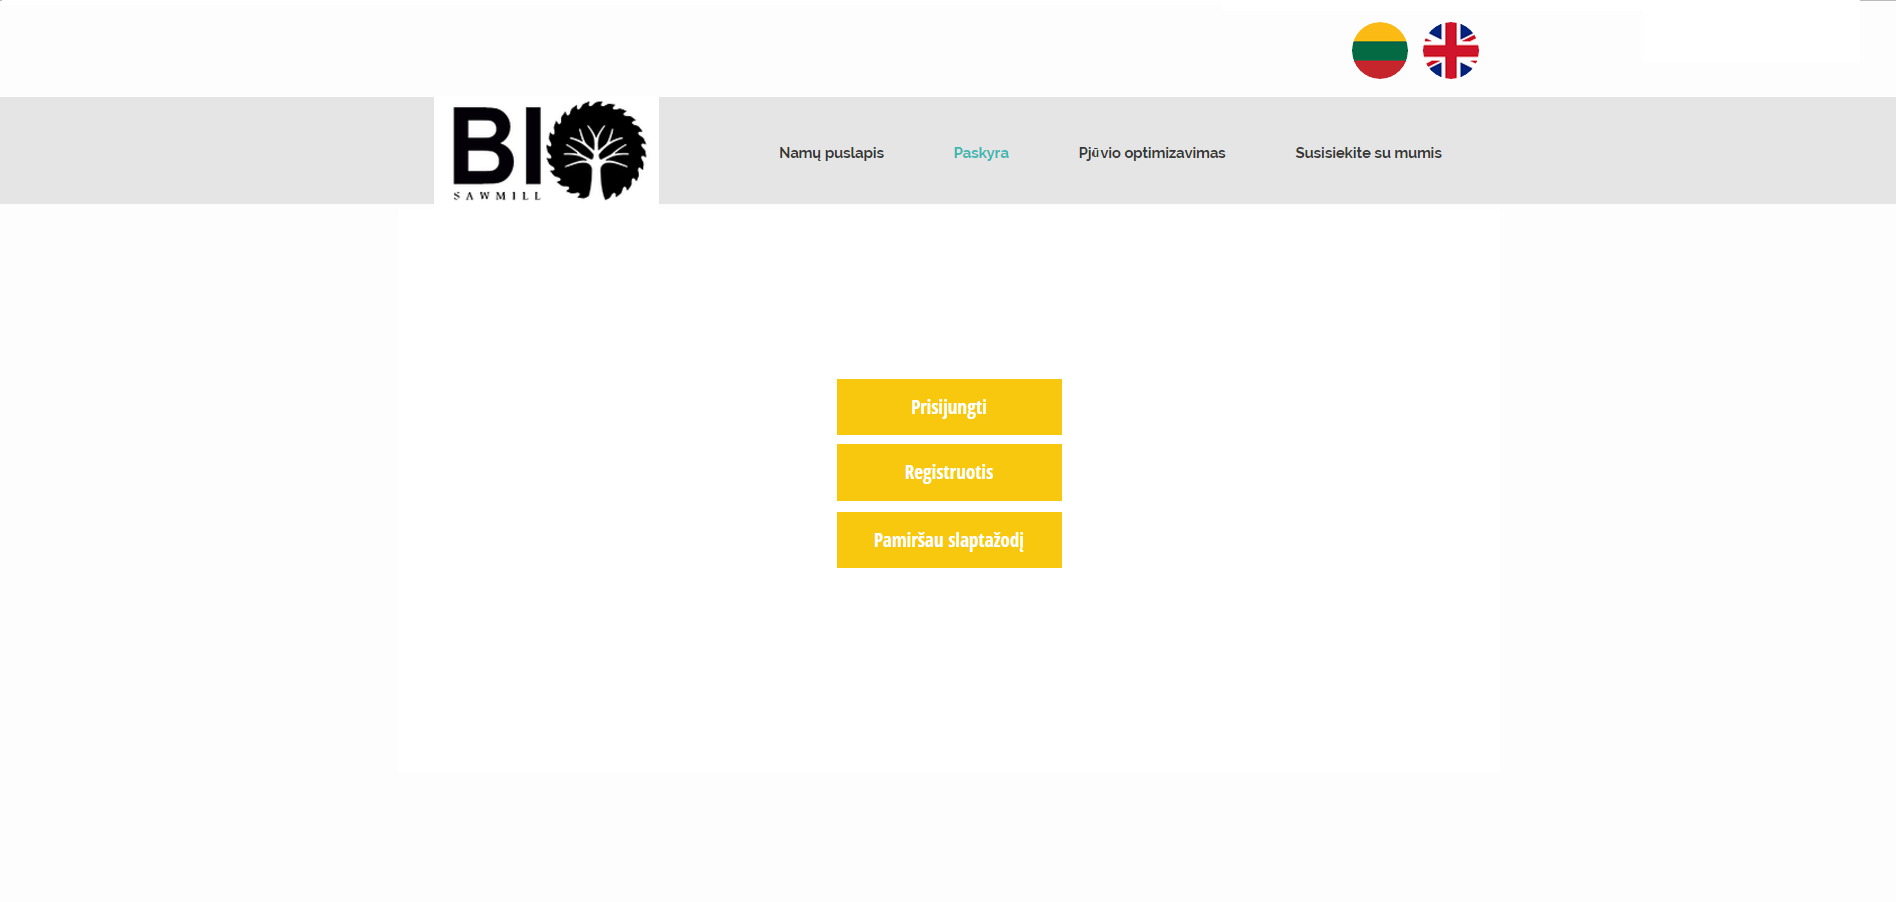
\includegraphics[scale=0.5]{interfeisai/paskyrosPuslapisNeprisijungta}

\subsection{Vartotojo paskyros puslapis - registracija}
\hspace{-2cm}
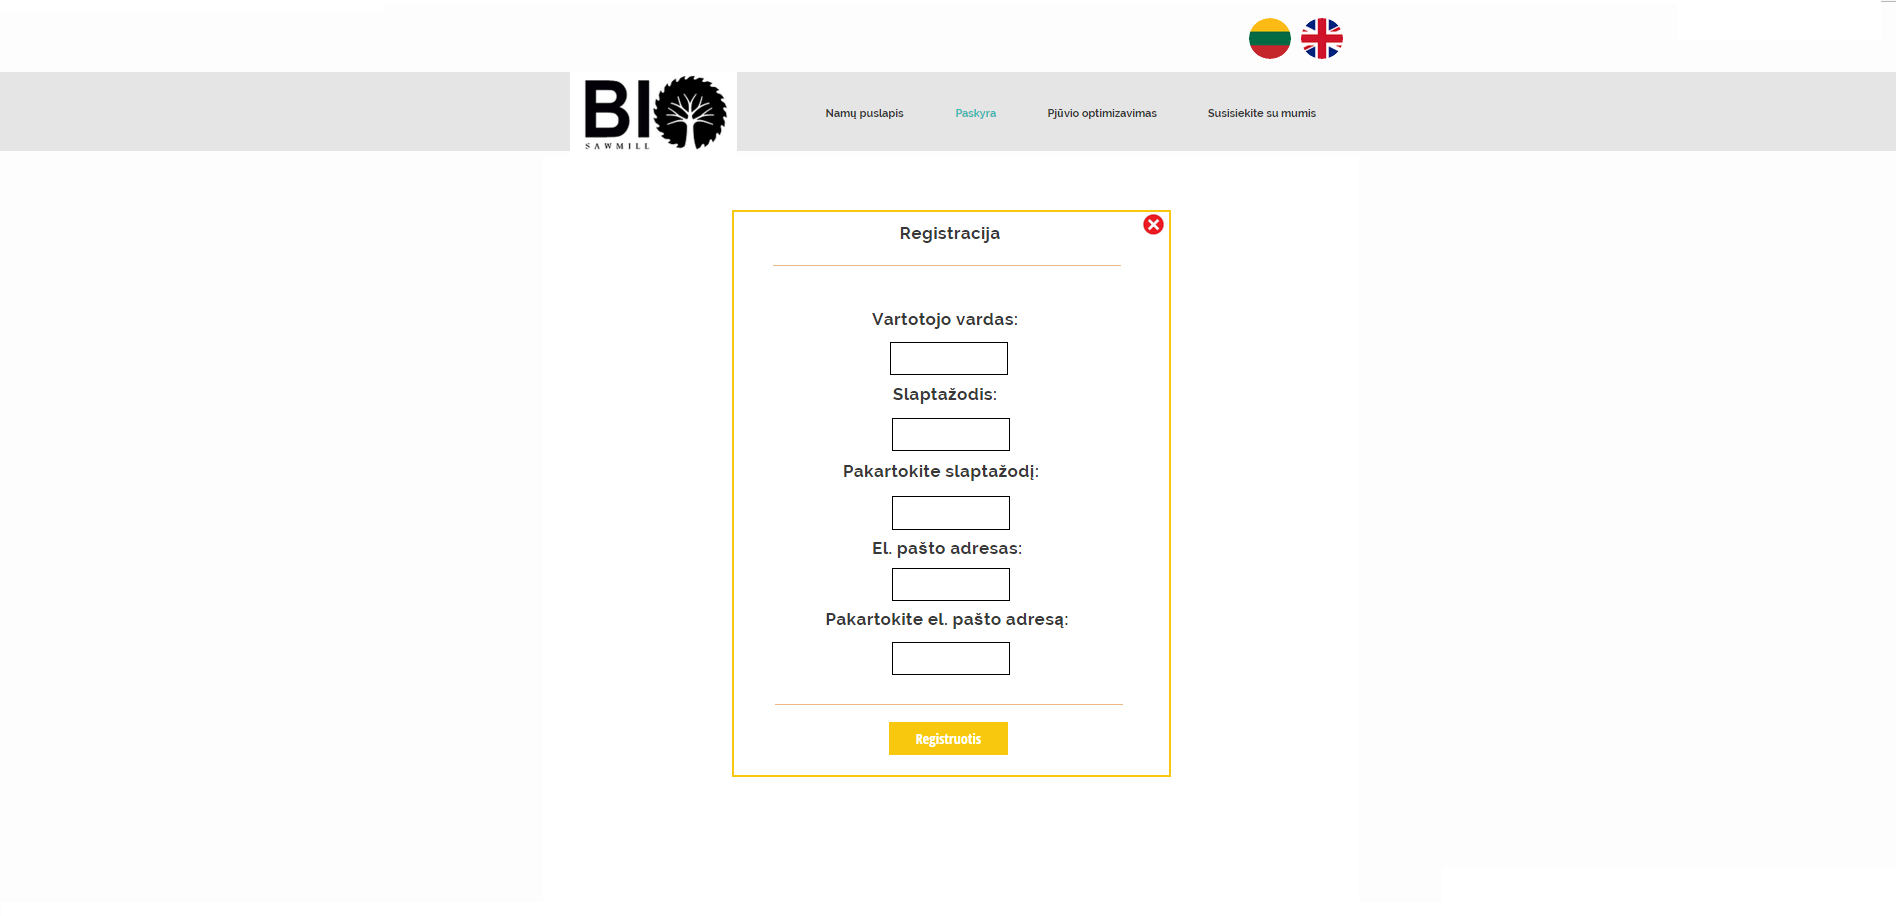
\includegraphics[scale=0.5]{interfeisai/paskyrosPuslapisRegistracija}

\subsection{Vartotojo paskyros puslapis - registracija (su klaida)}
\hspace{-2cm}
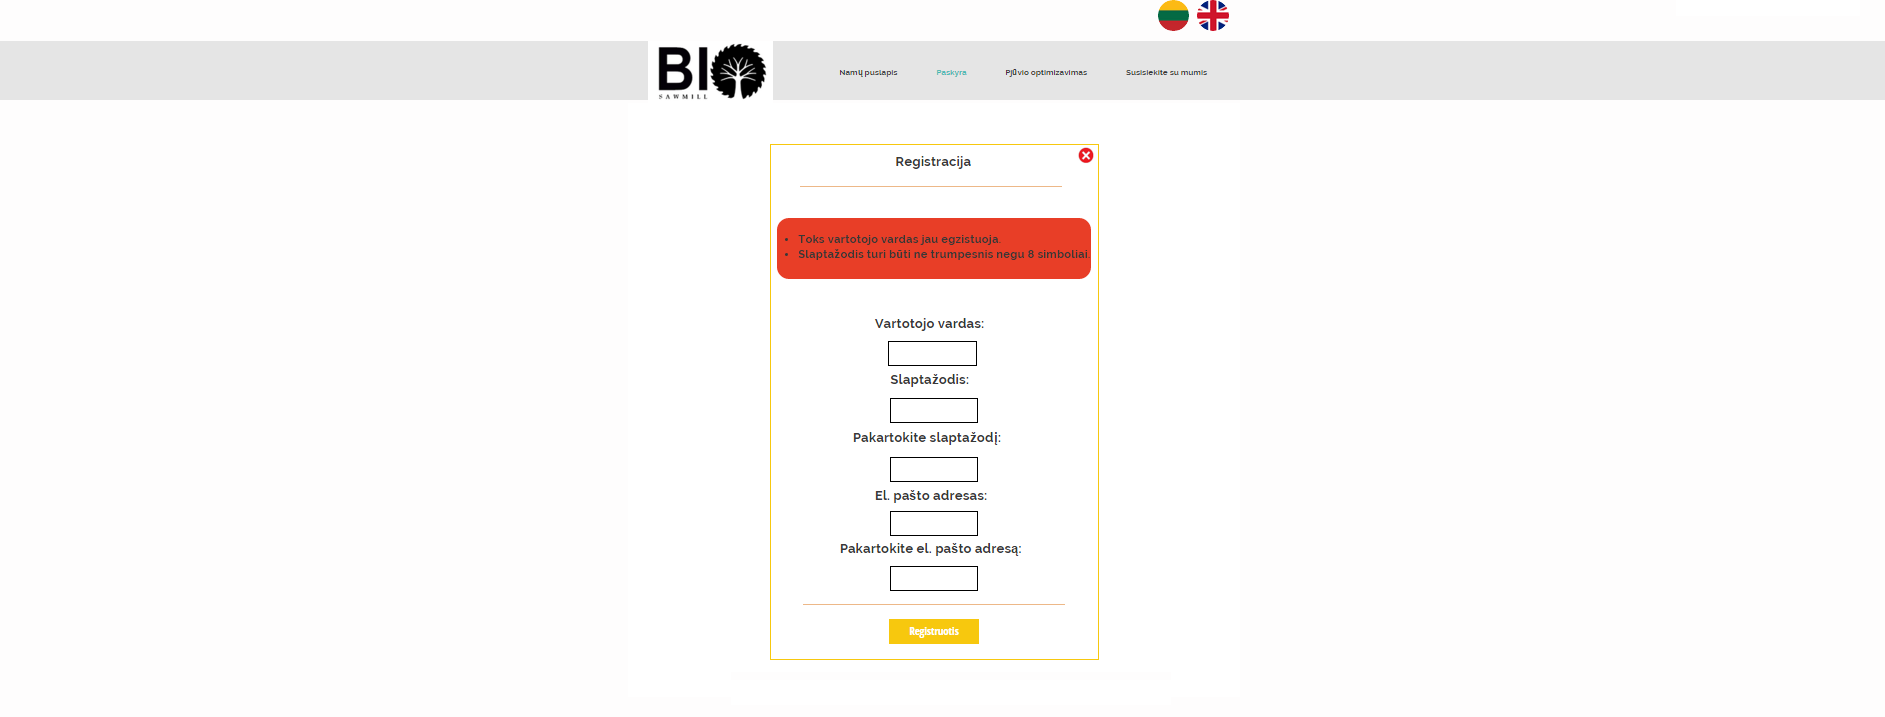
\includegraphics[scale=0.5]{interfeisai/paskyrosPuslapisRegistracijaSuKlaida}

\subsection{Vartotojo paskyros puslapis - sėkminga registracija}
\hspace{-2cm}
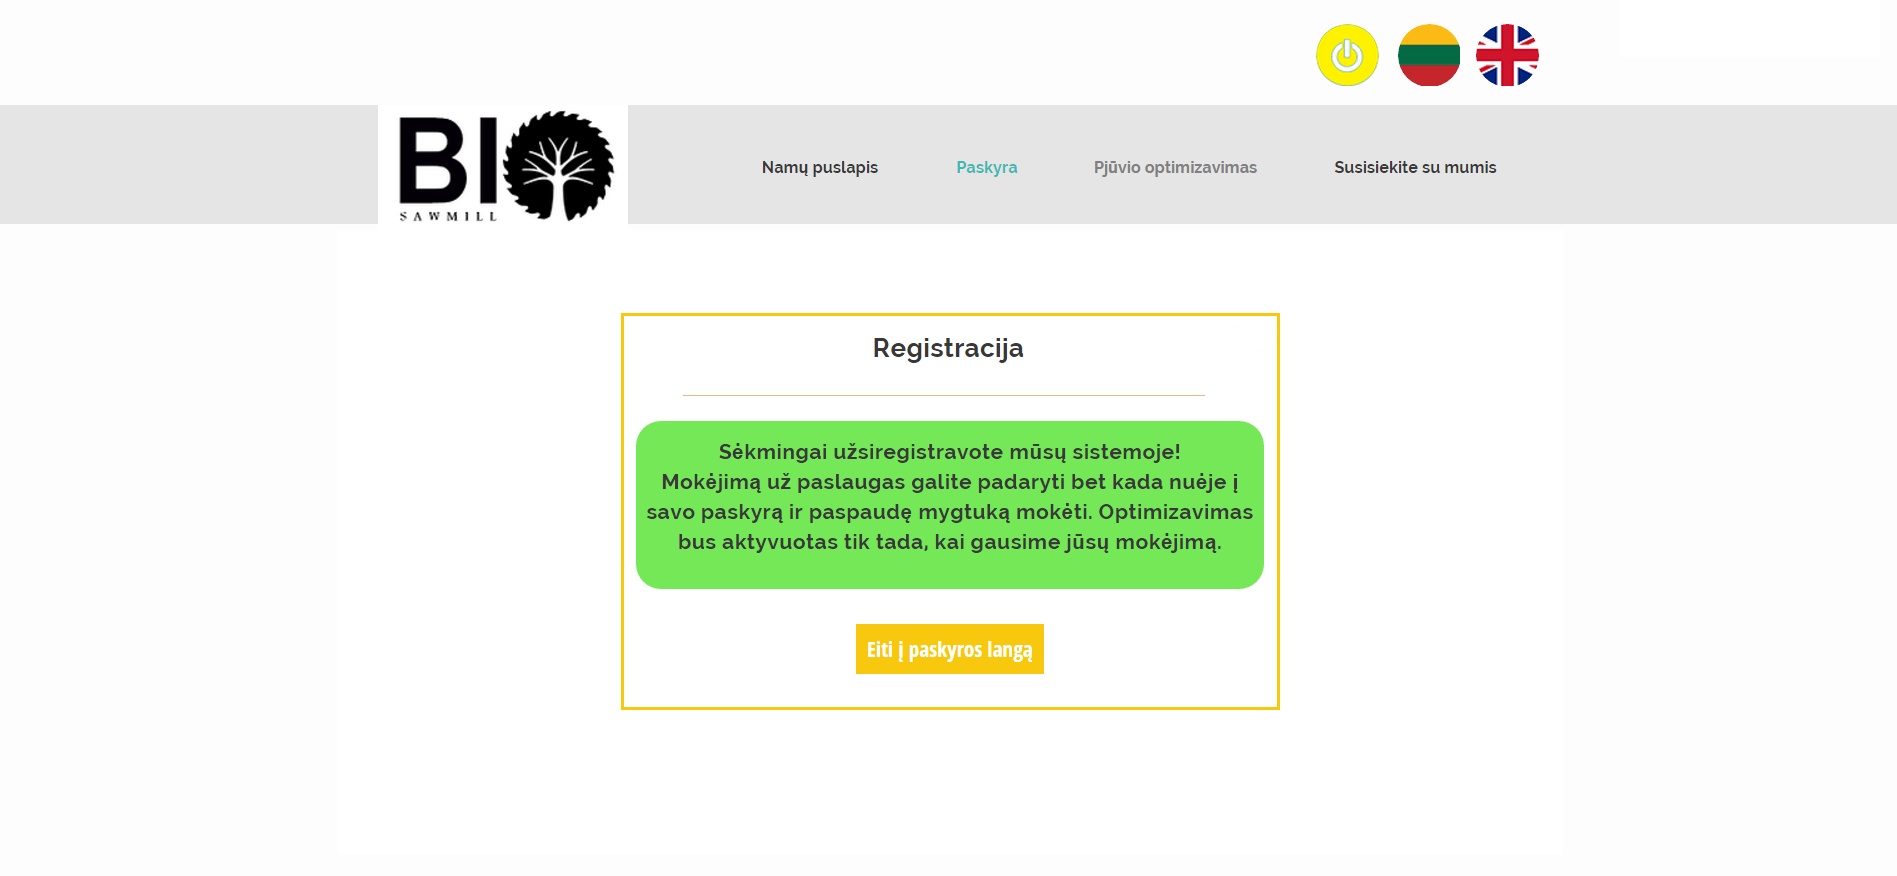
\includegraphics[scale=0.5]{interfeisai/paskyrosPuslapisRegistracijaSekminga}

\subsection{Vartotojo paskyros puslapis - prisijungimas}
\hspace{-2cm}
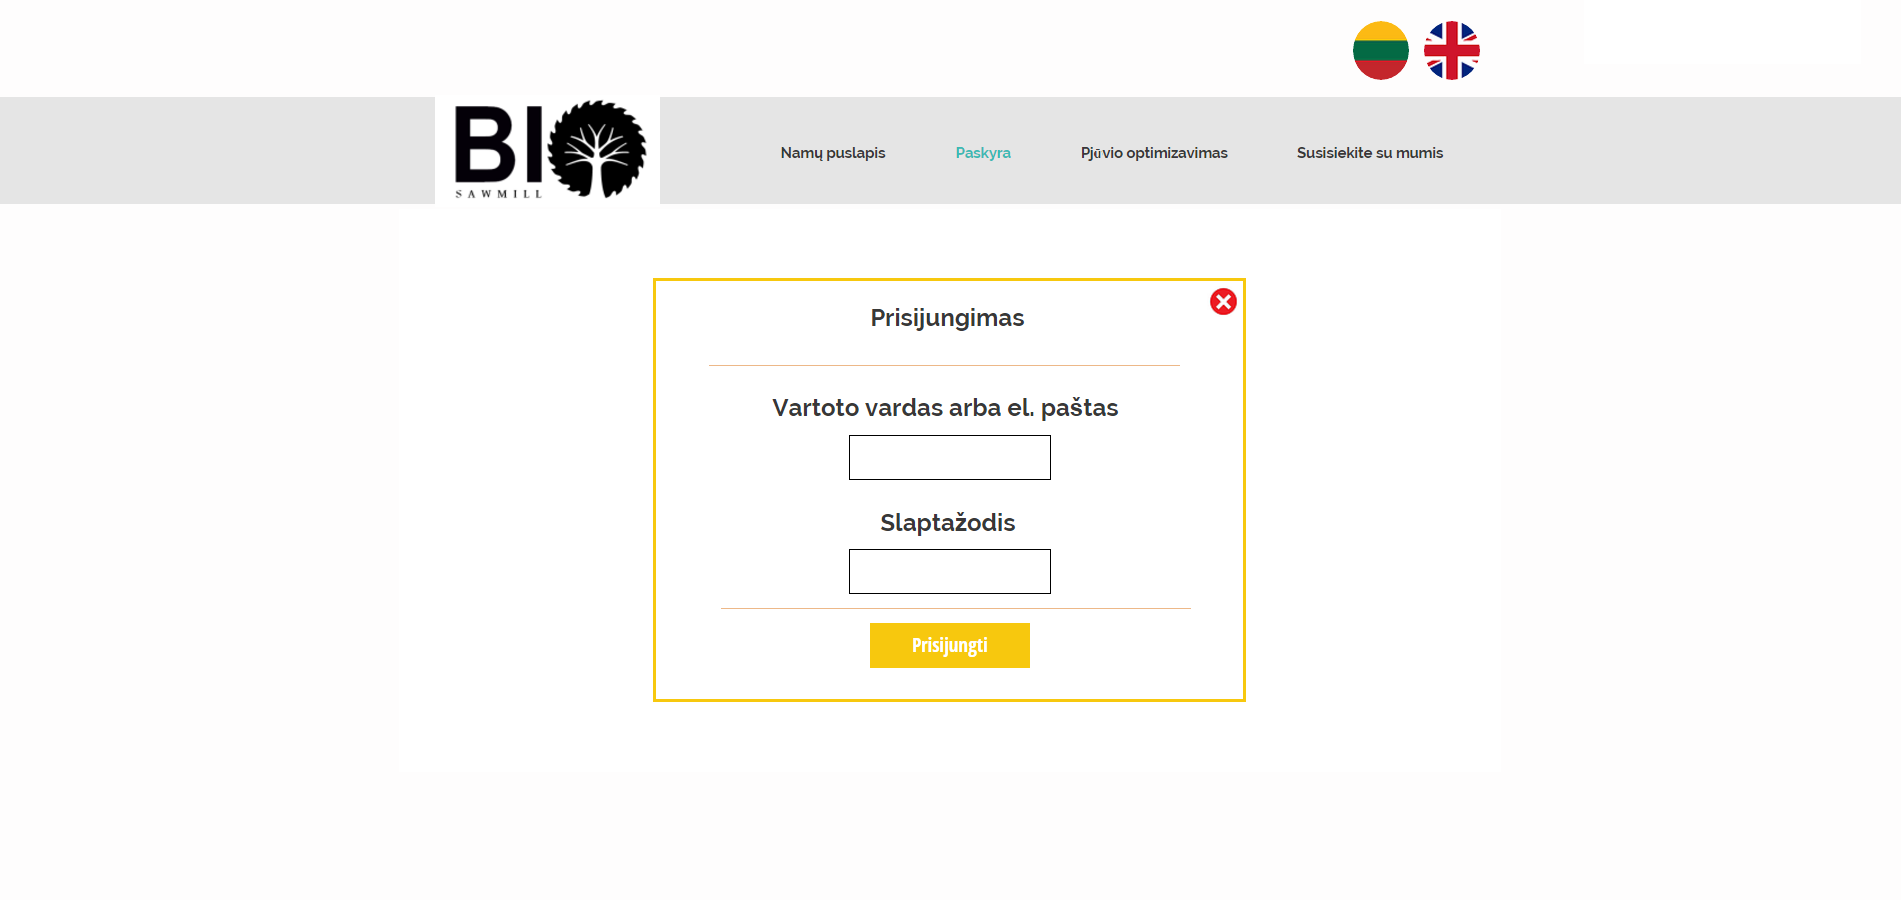
\includegraphics[scale=0.5]{interfeisai/paskyrosPuslapisPrisijungimas}

\subsection{Vartotojo paskyros puslapis - prisijungimas (su klaida)}
\hspace{-2cm}
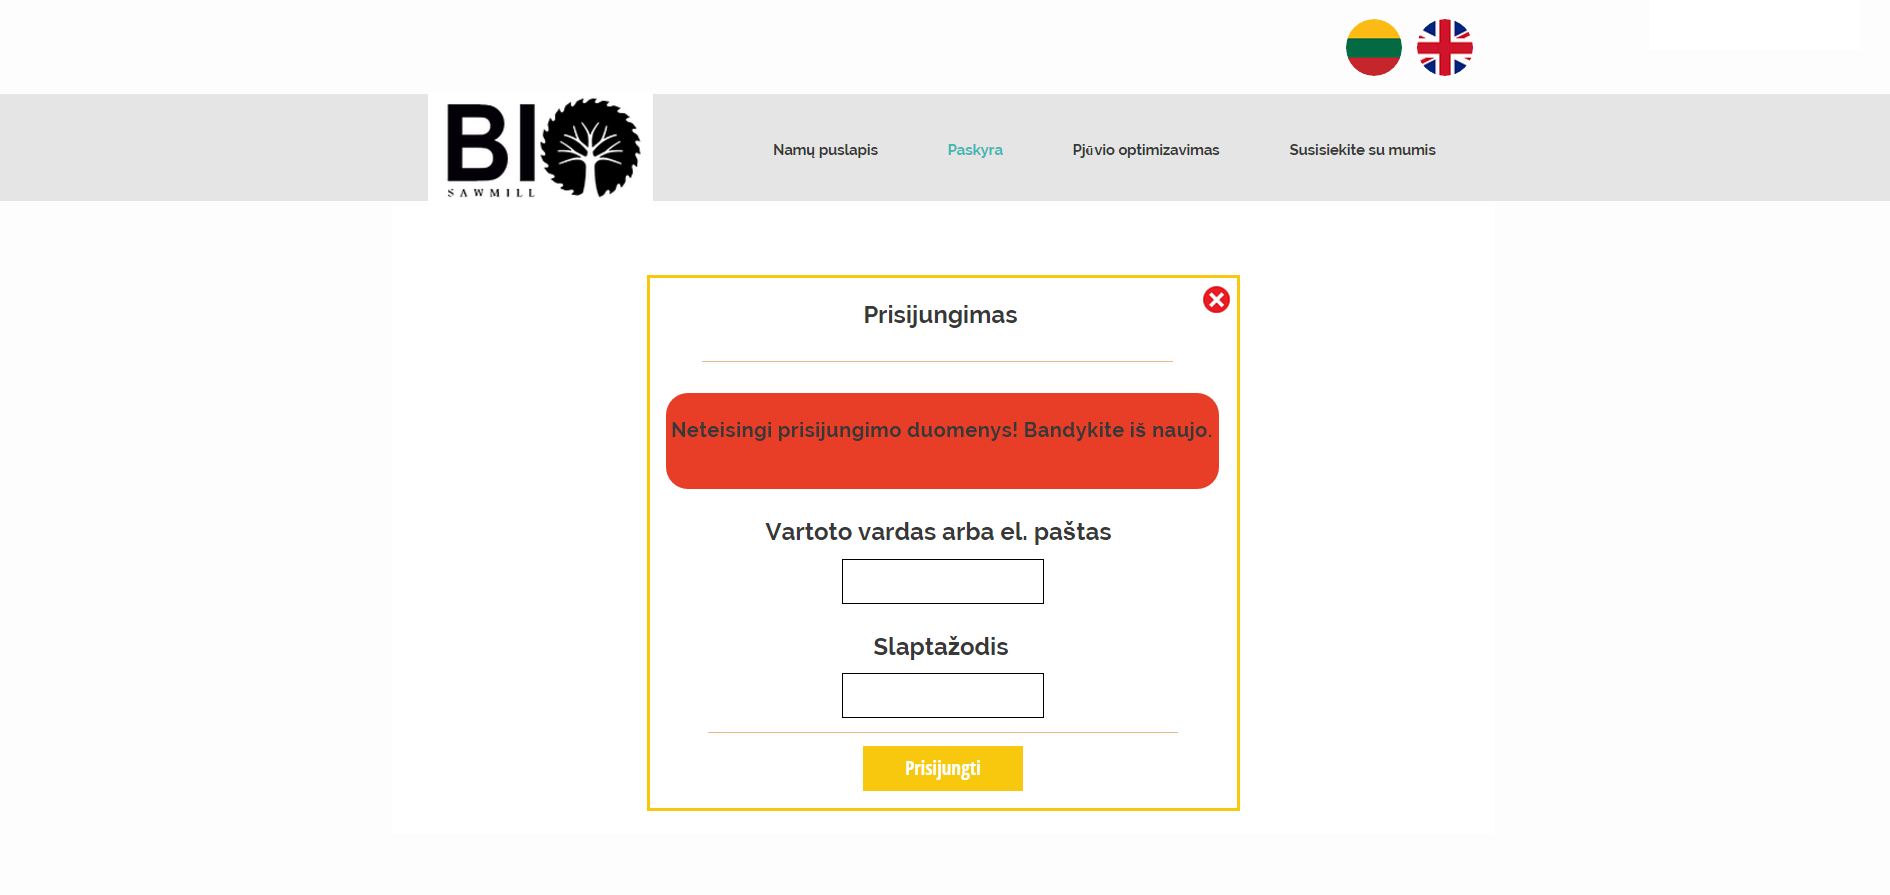
\includegraphics[scale=0.5]{interfeisai/paskyrosPuslapisPrisijungimasSuKlaida}

\subsection{Vartotojo paskyros puslapis - pamirštas slaptažodis}
\hspace{-2cm}
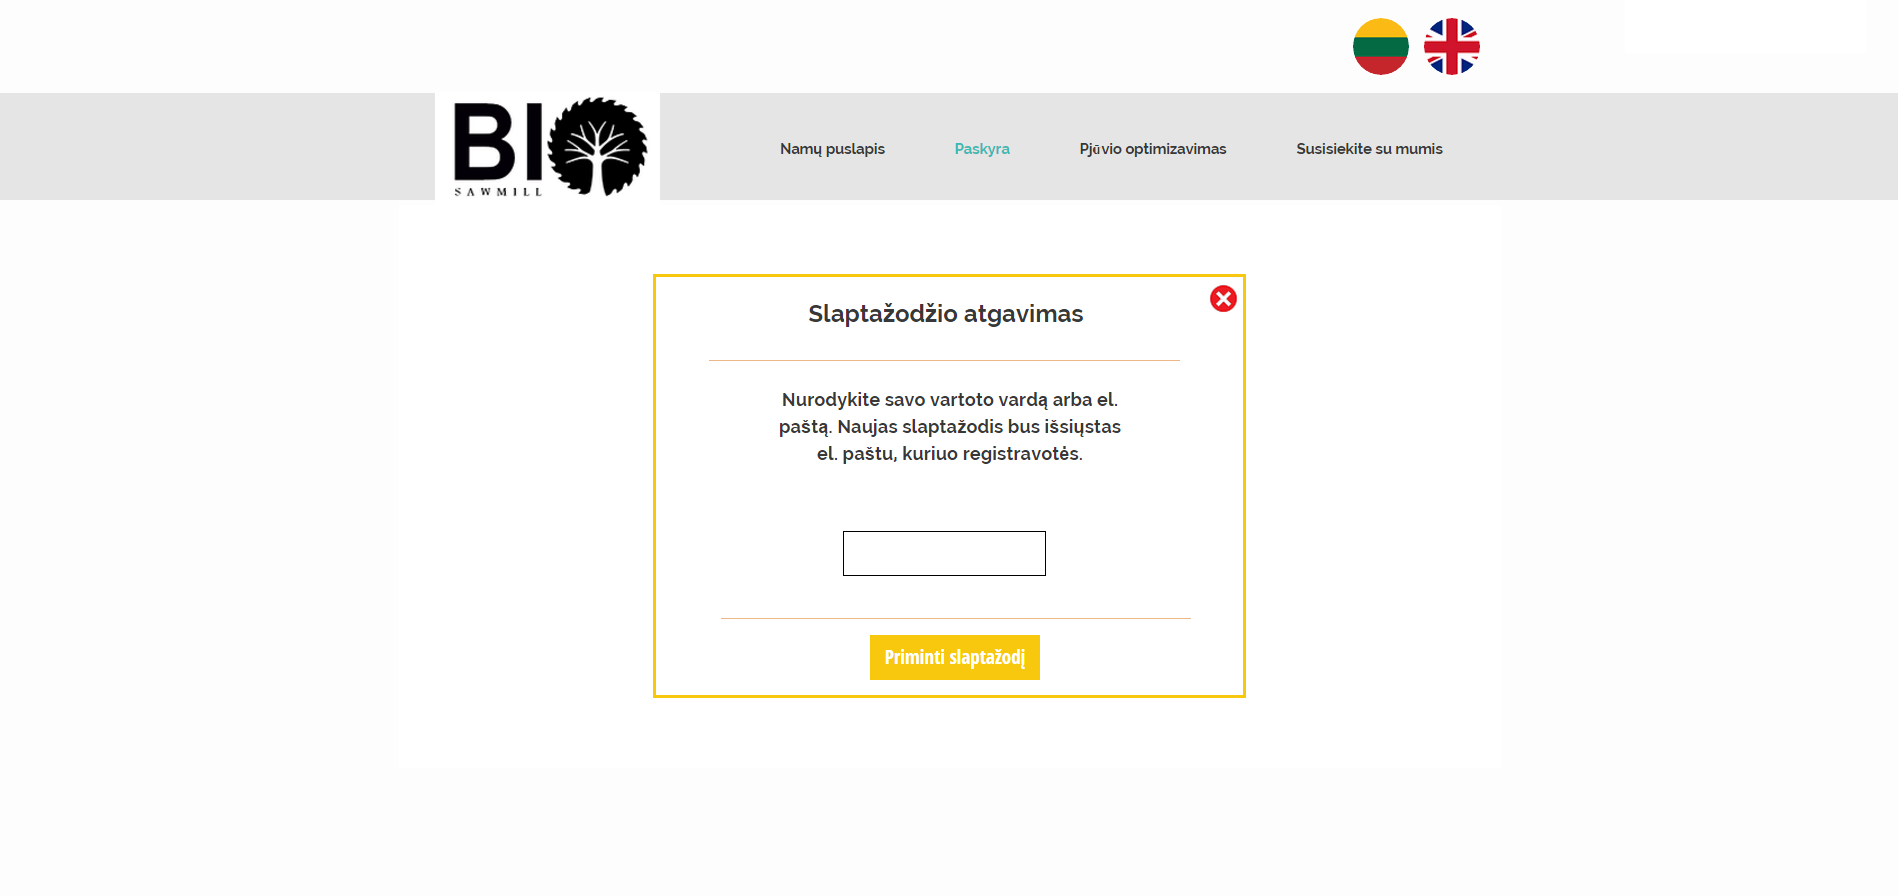
\includegraphics[scale=0.5]{interfeisai/paskyrosPuslapisPamirstasSlaptazodis}

\subsection{Vartotojo paskyros puslapis - pamirštas slaptažodis 2}
\hspace{-2cm}
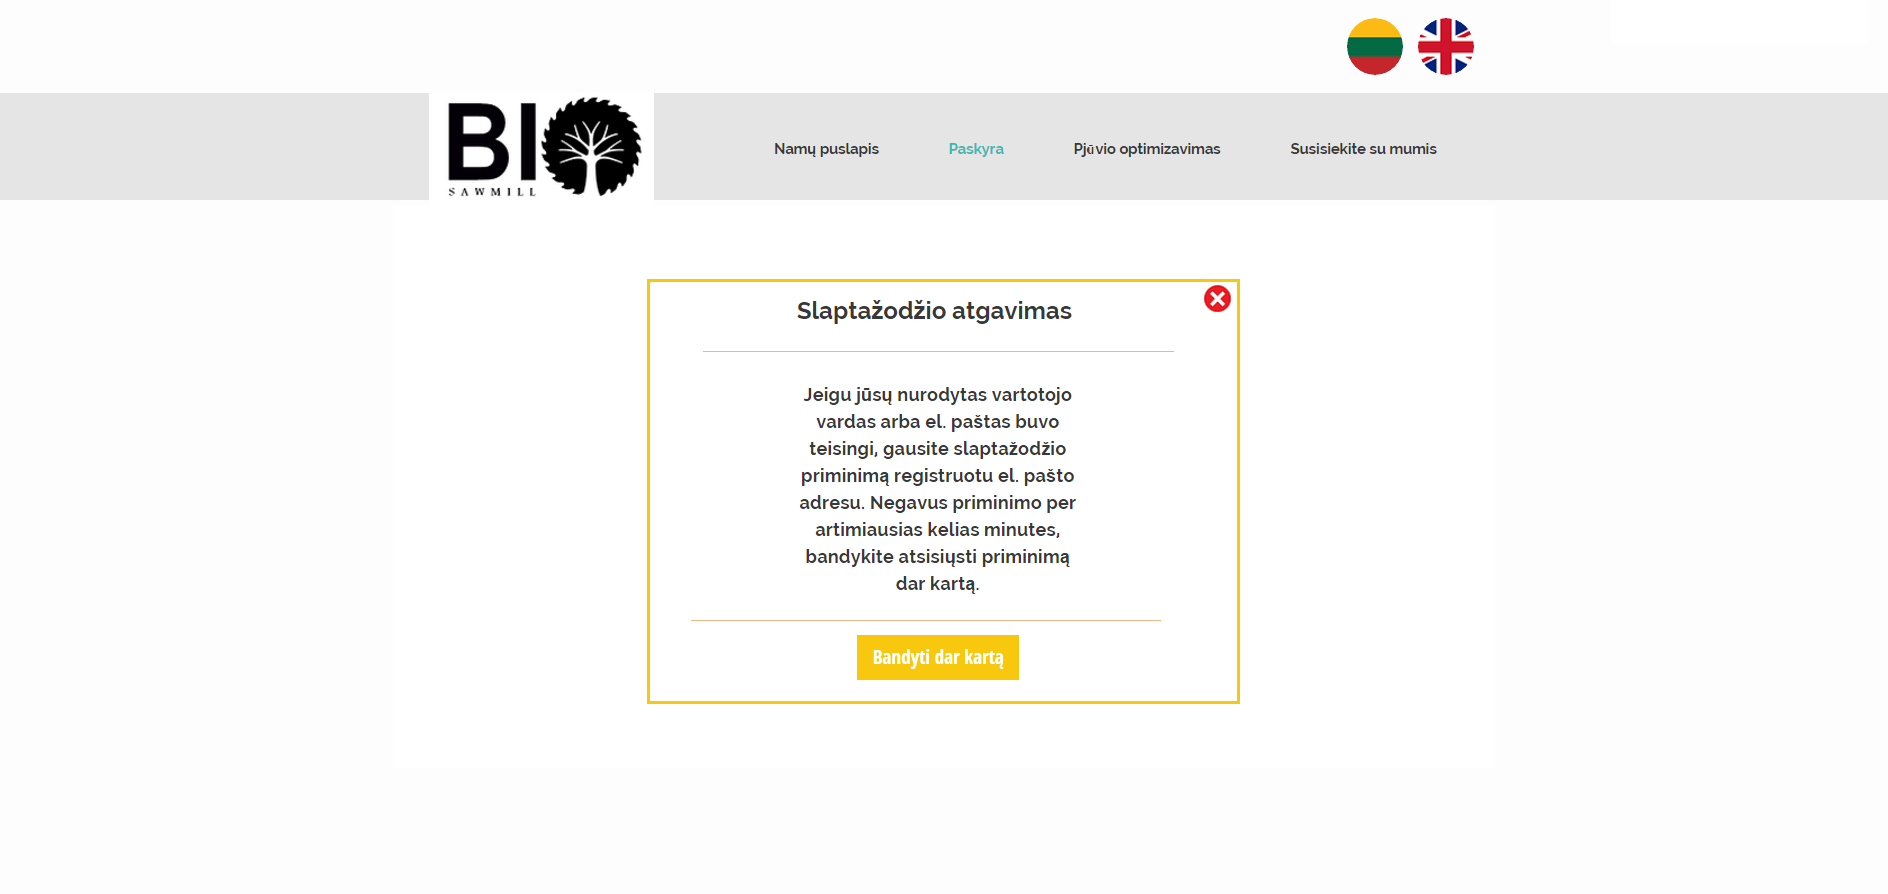
\includegraphics[scale=0.5]{interfeisai/paskyrosPuslapisPamirstasSlaptazodis2}

\subsection{Vartotojo paskyros puslapis - prisijungus (neapmokėta už paslaugas)}
\hspace{-2cm}
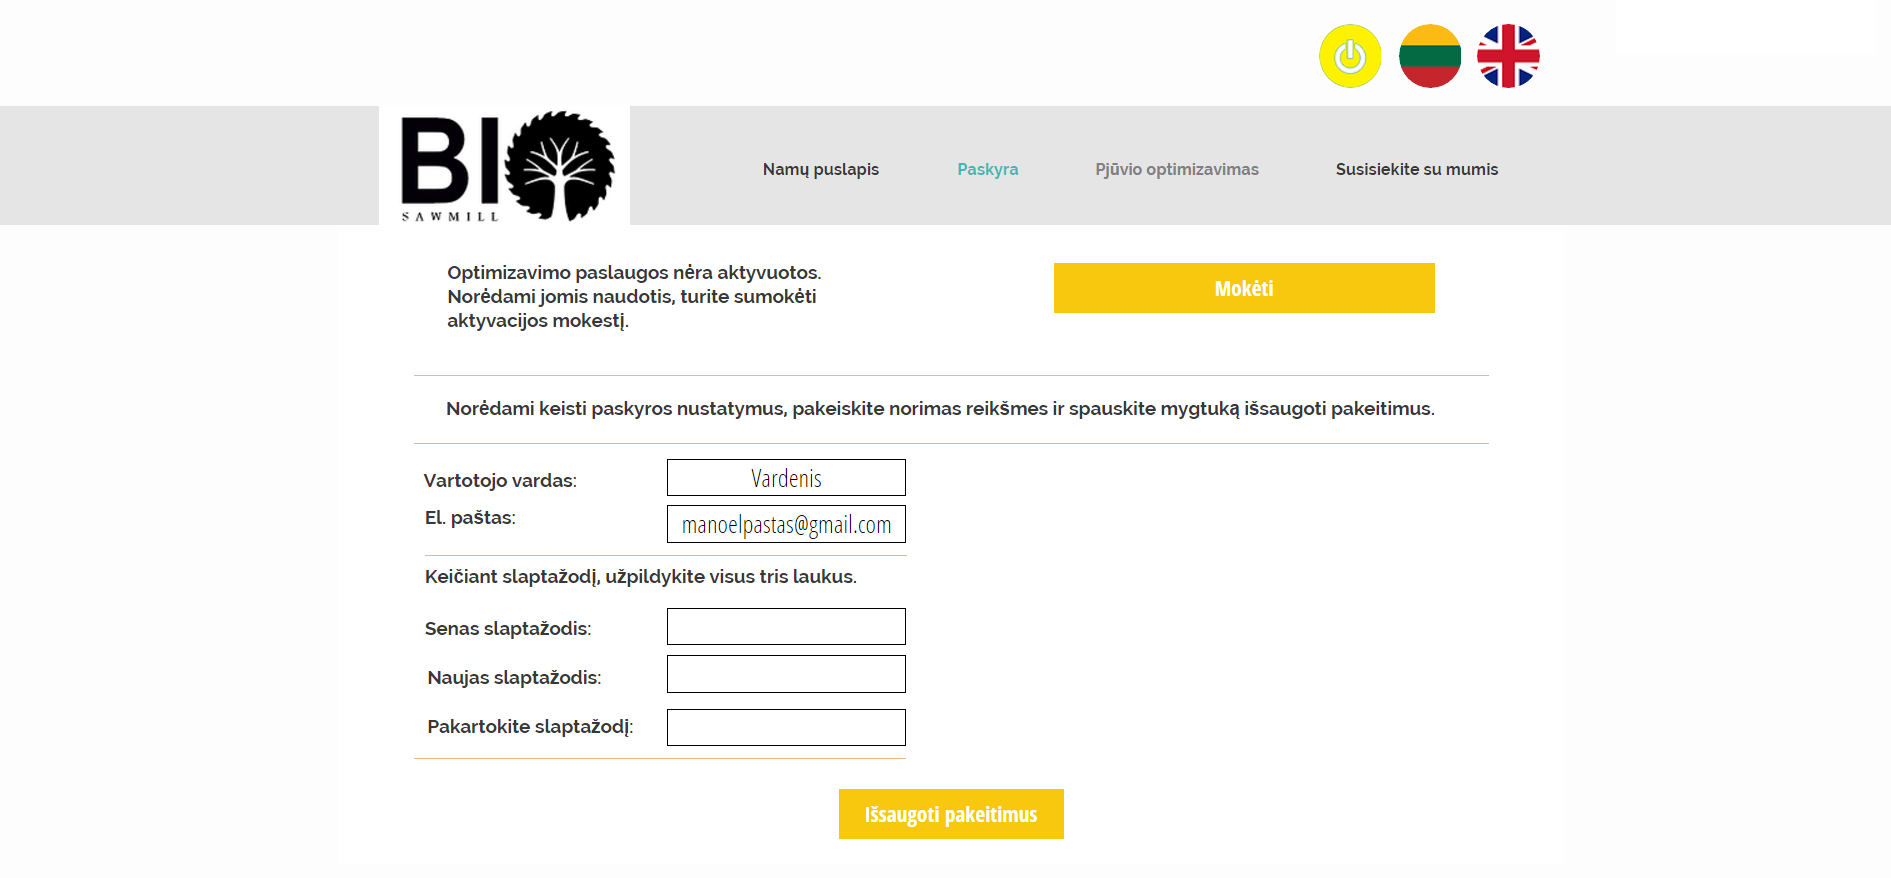
\includegraphics[scale=0.5]{interfeisai/paskyrosPuslapisVartotojasNeapmoketas}

\subsection{Vartotojo paskyros puslapis - prisijungus (apmokėta už paslaugas)}
\hspace{-2cm}
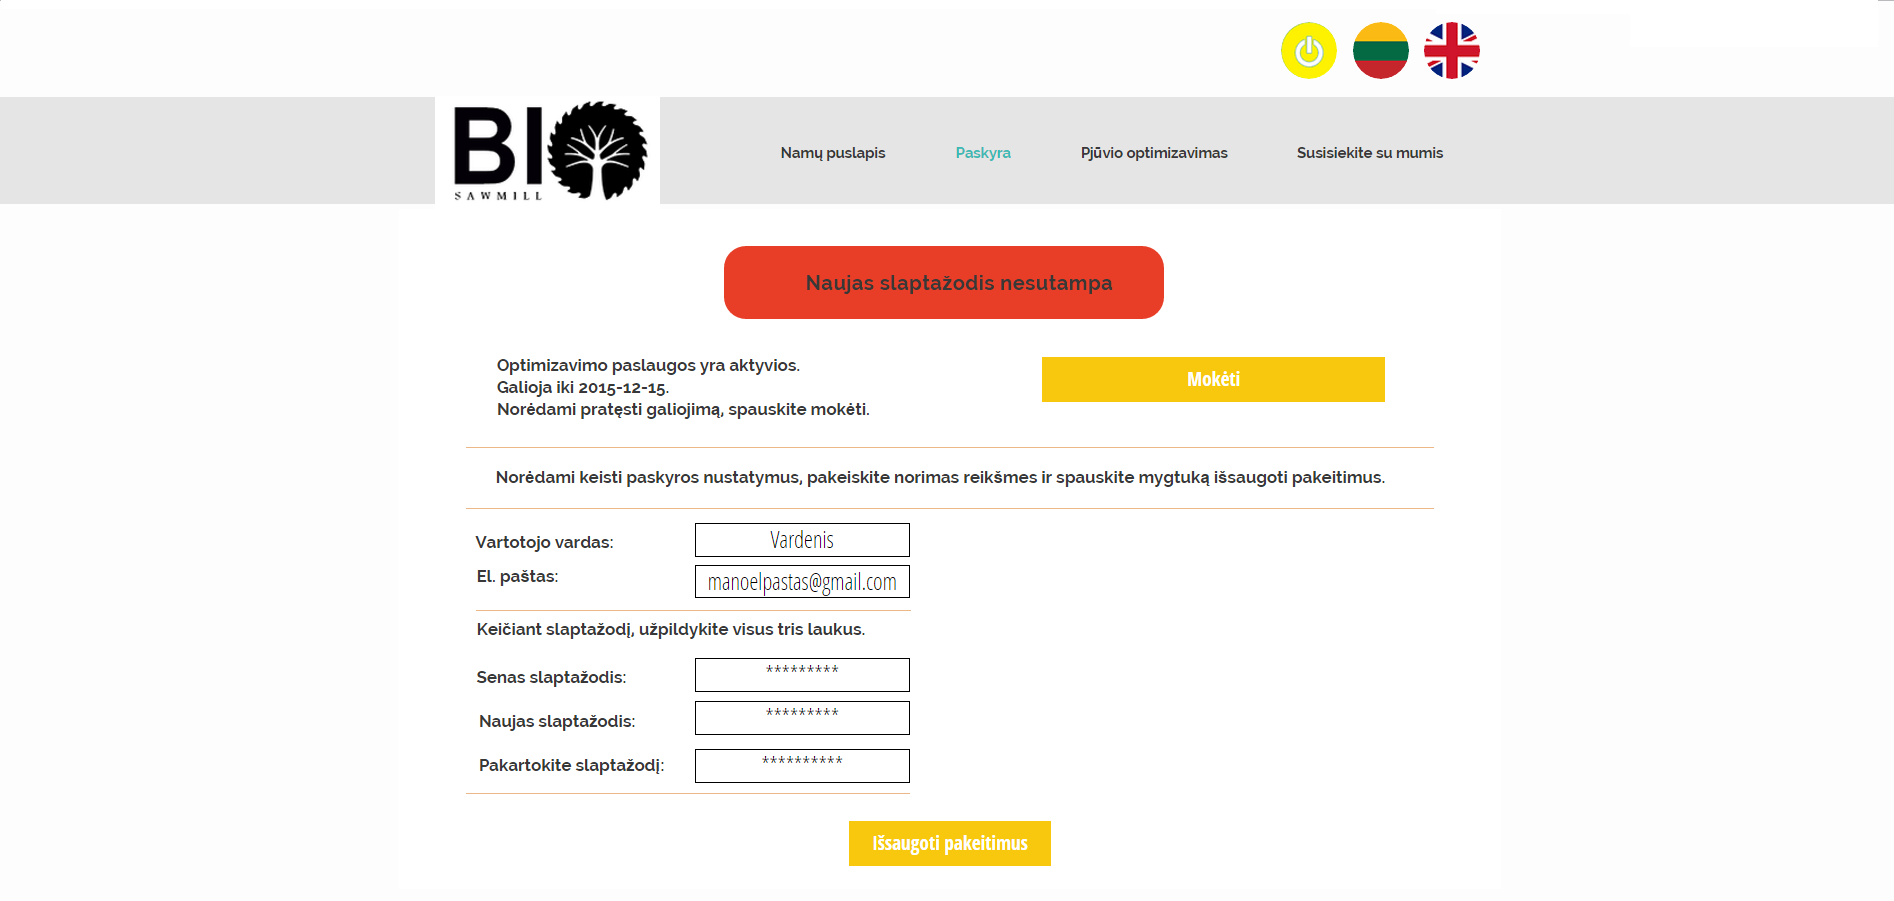
\includegraphics[scale=0.5]{interfeisai/paskyrosPuslapisVartotojasApmoketas}

\subsection{Vartotojo paskyros puslapis - prisijungus - mokėjimas}
\hspace{-2cm}
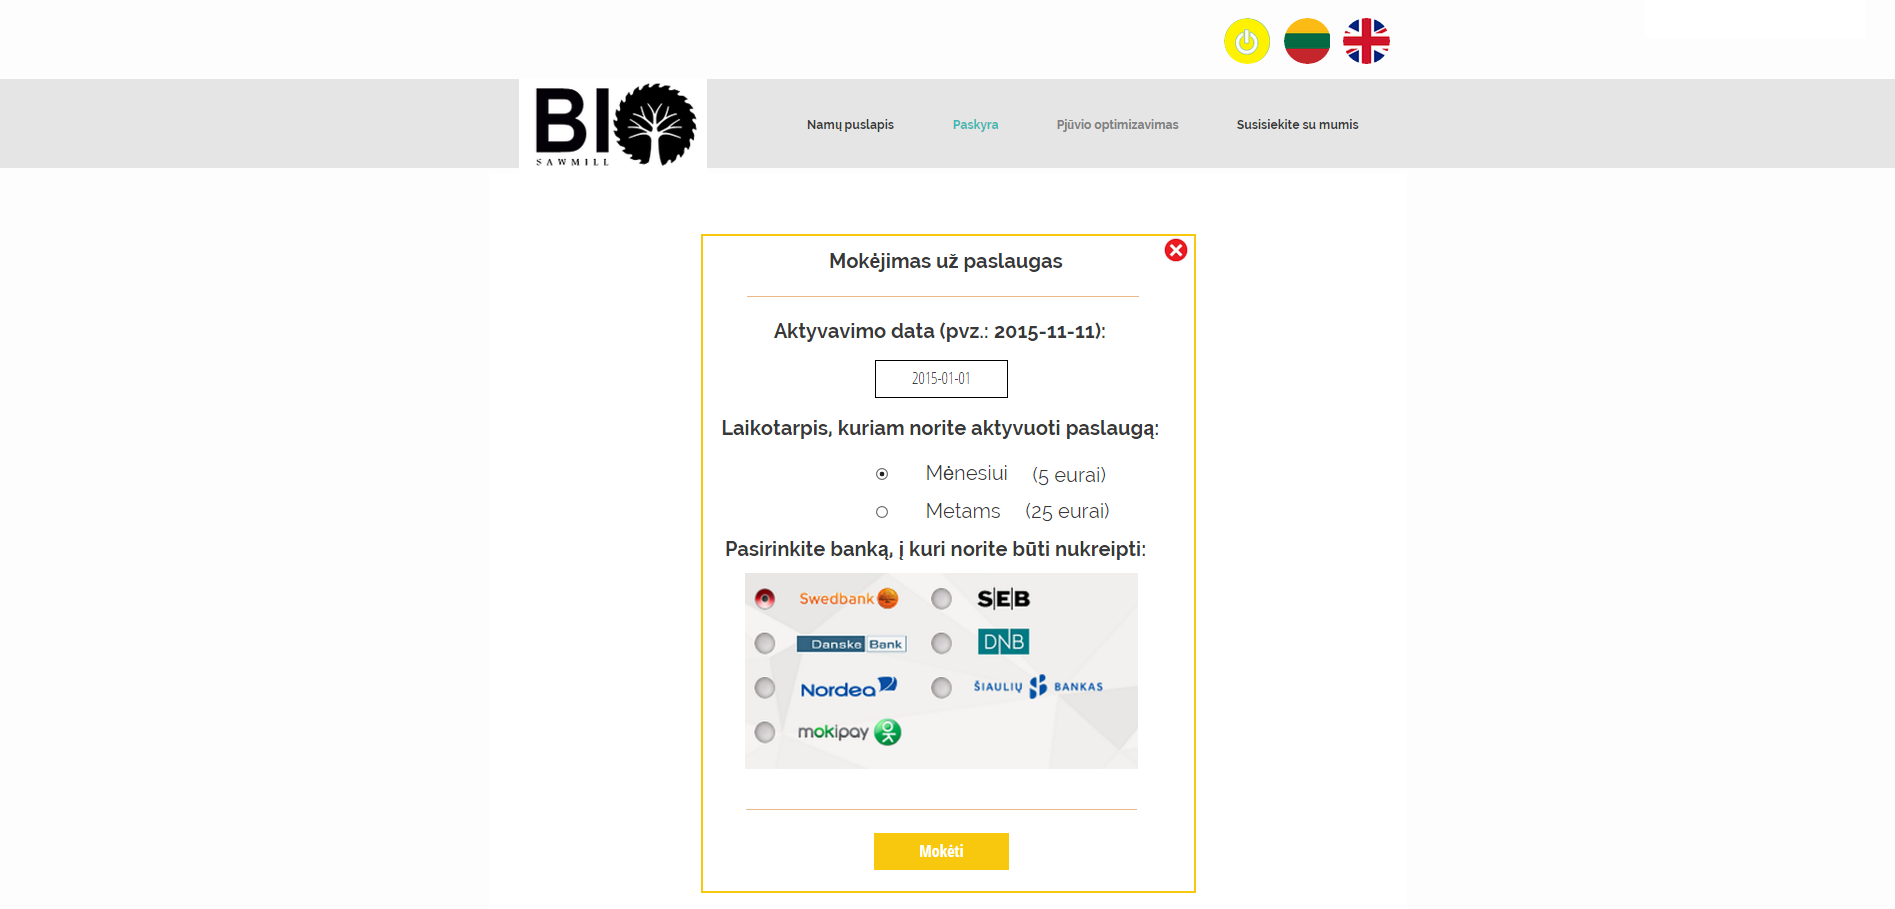
\includegraphics[scale=0.5]{interfeisai/paskyrosPuslapisVartotojasMokejimas}

\subsection{Vartotojo paskyros puslapis - prisijungus - mokėjimas (su klaida)}
\hspace{-2cm}
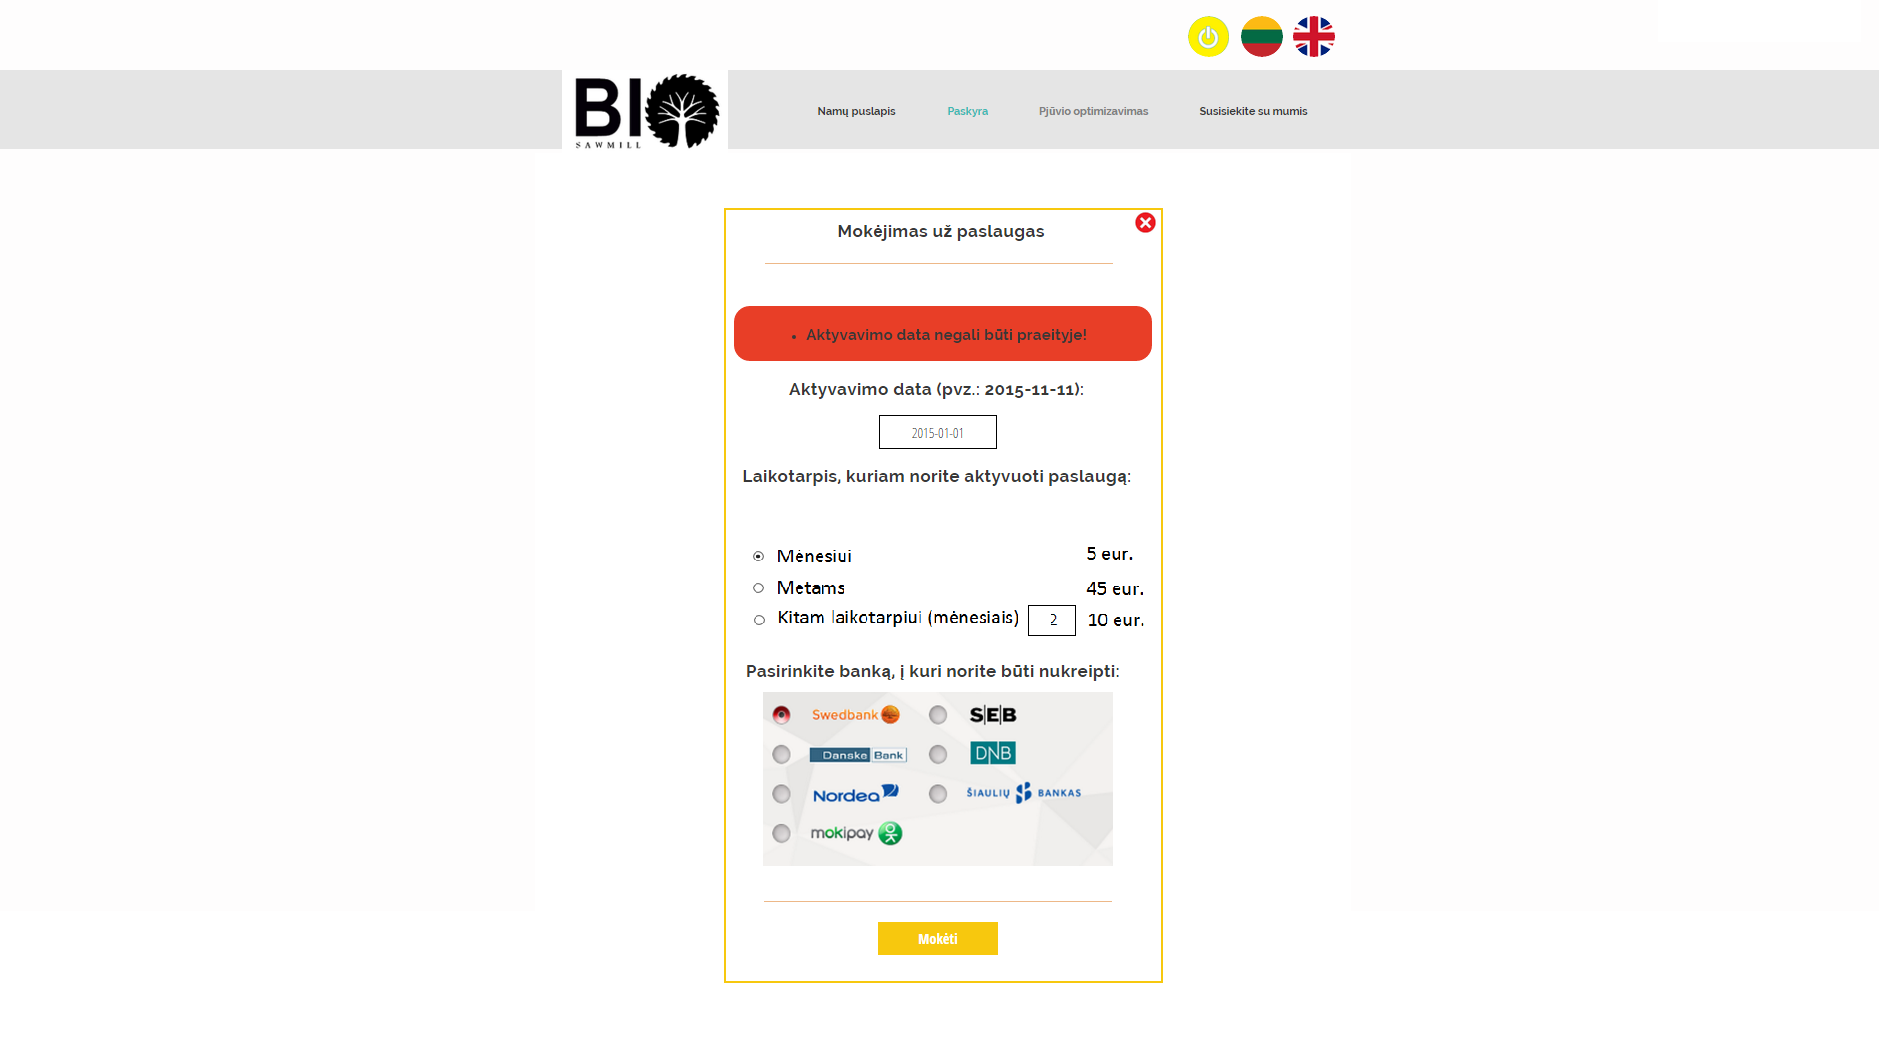
\includegraphics[scale=0.5]{interfeisai/paskyrosPuslapisVartotojasMokejimasSuKlaida}

\subsection{Vartotojo paskyros puslapis - administratorius}
\hspace{-2cm}
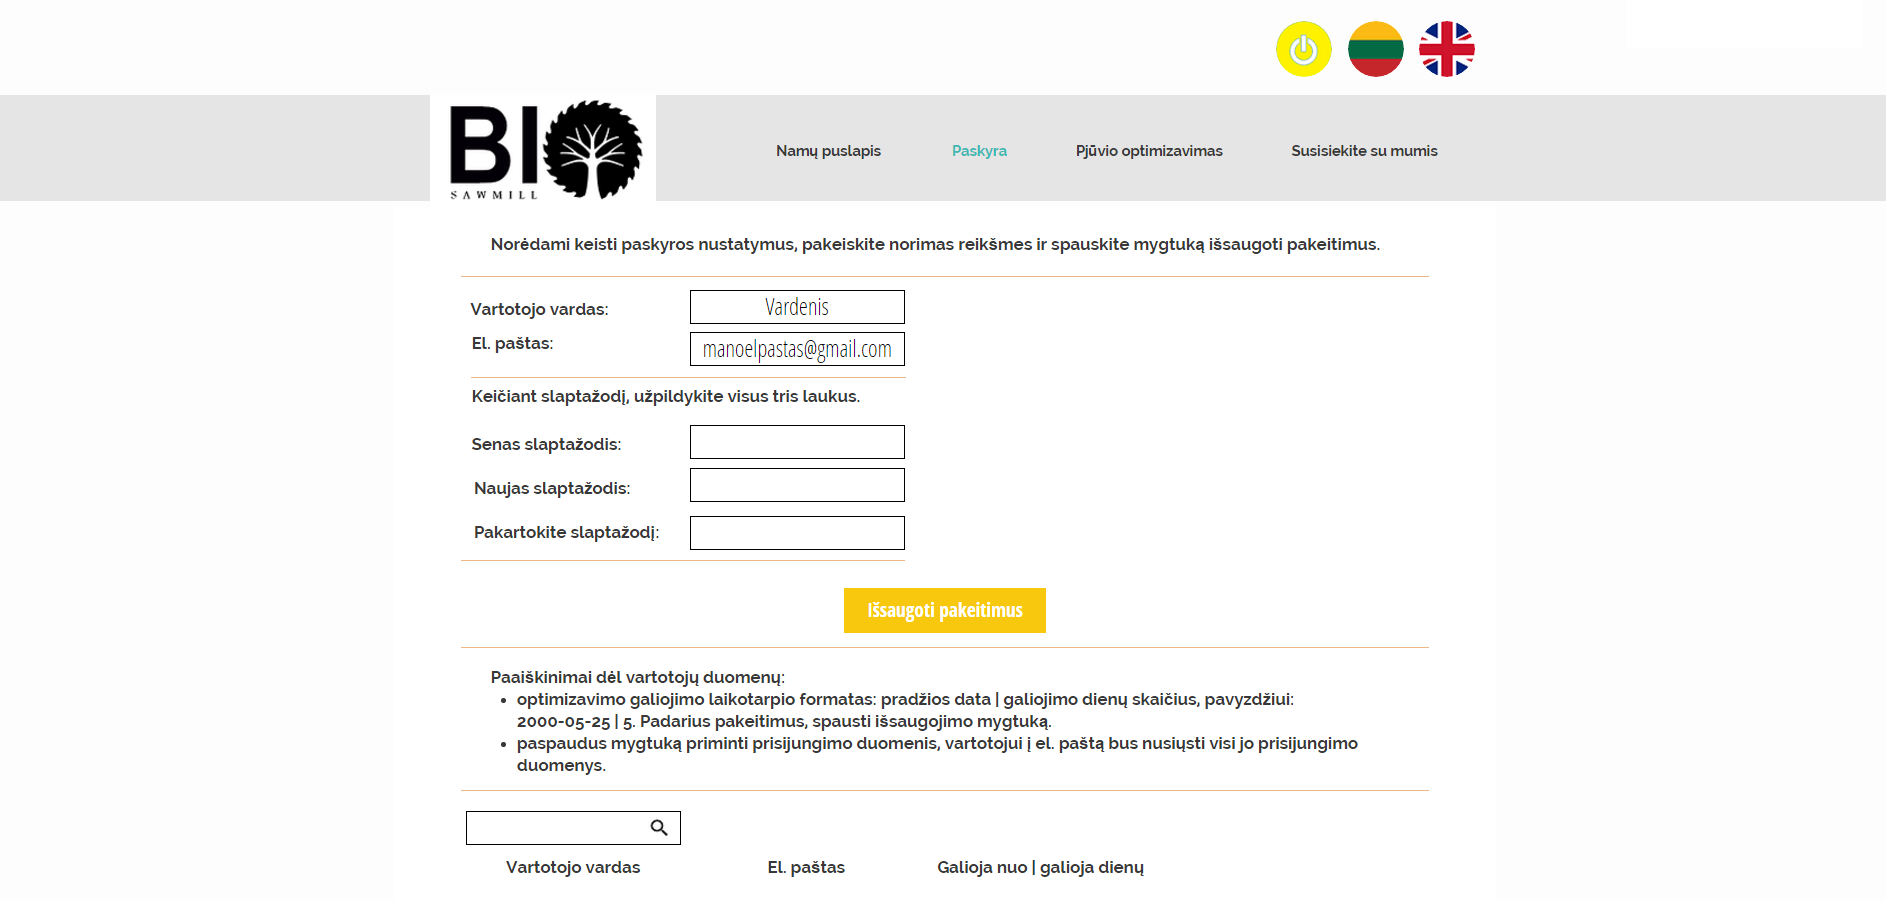
\includegraphics[scale=0.5]{interfeisai/paskyrosPuslapisAdministratorius}

\subsection{Vartotojo paskyros puslapis - administratorius (su klaida)}
\hspace{-2cm}
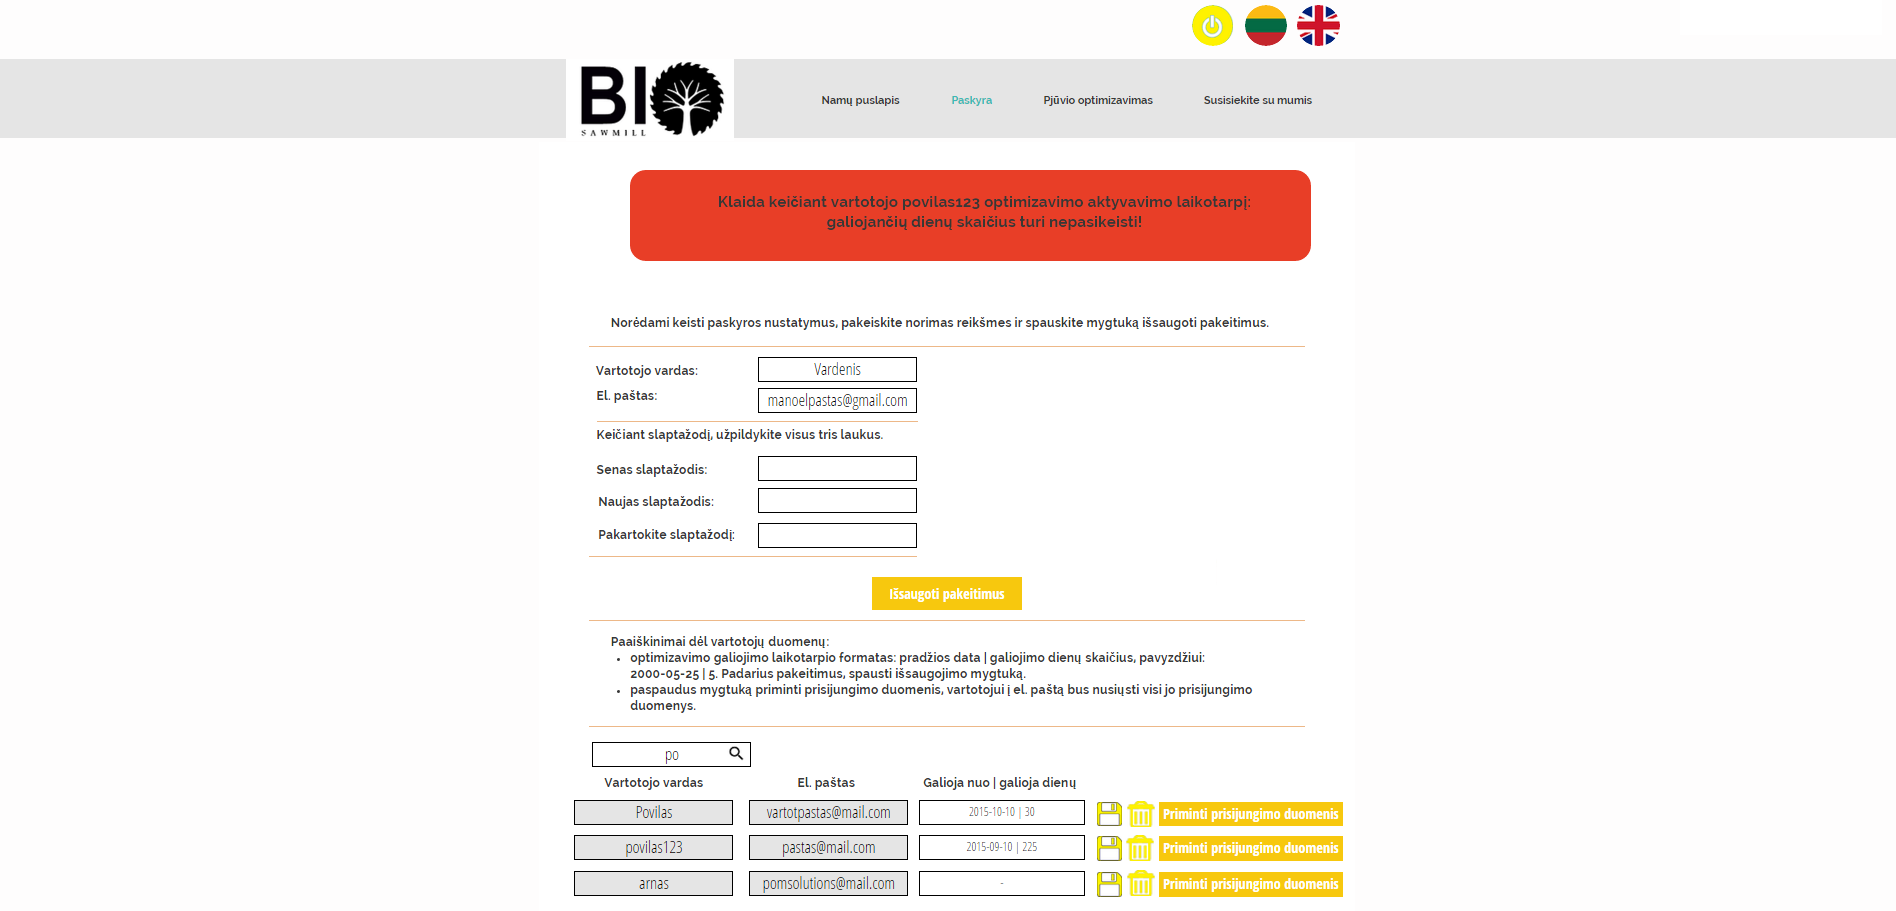
\includegraphics[scale=0.5]{interfeisai/paskyrosPuslapisAdministratoriusSuKlaida}

\subsection{Optimizavimo puslapis - neprisijungus}
\hspace{-2cm}
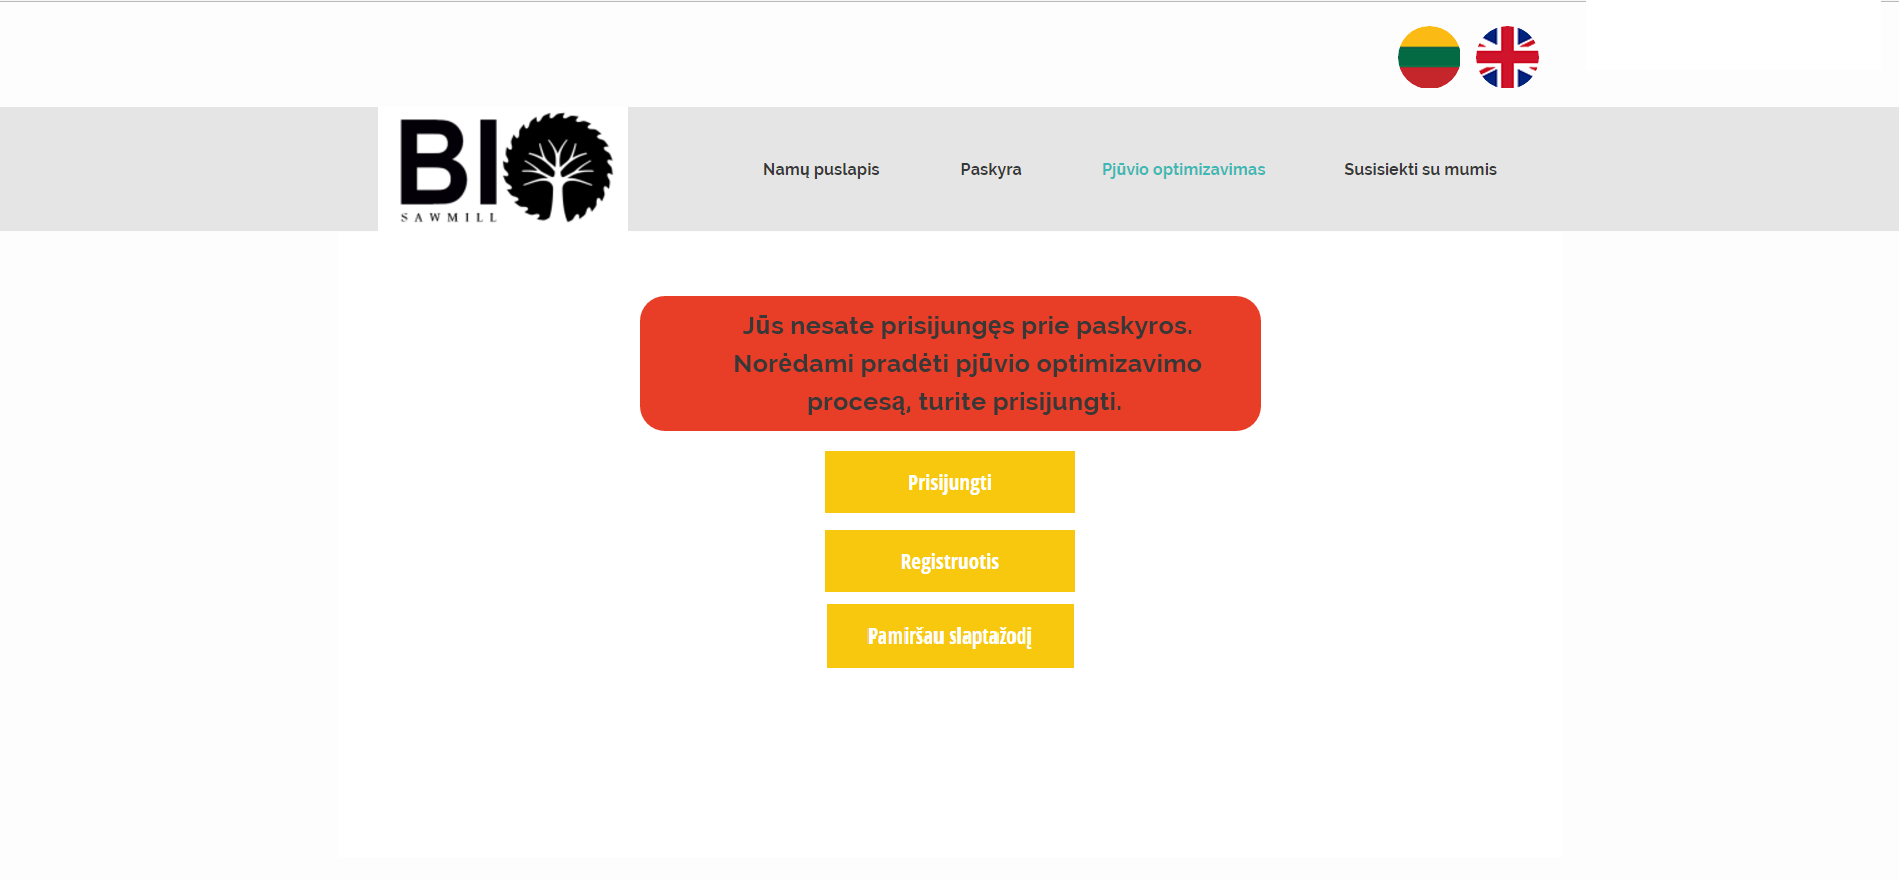
\includegraphics[scale=0.5]{interfeisai/optimizavimoPuslapisNeprisijungus}

\subsection{Optimizavimo puslapis - prisijungus}
\hspace{-2cm}
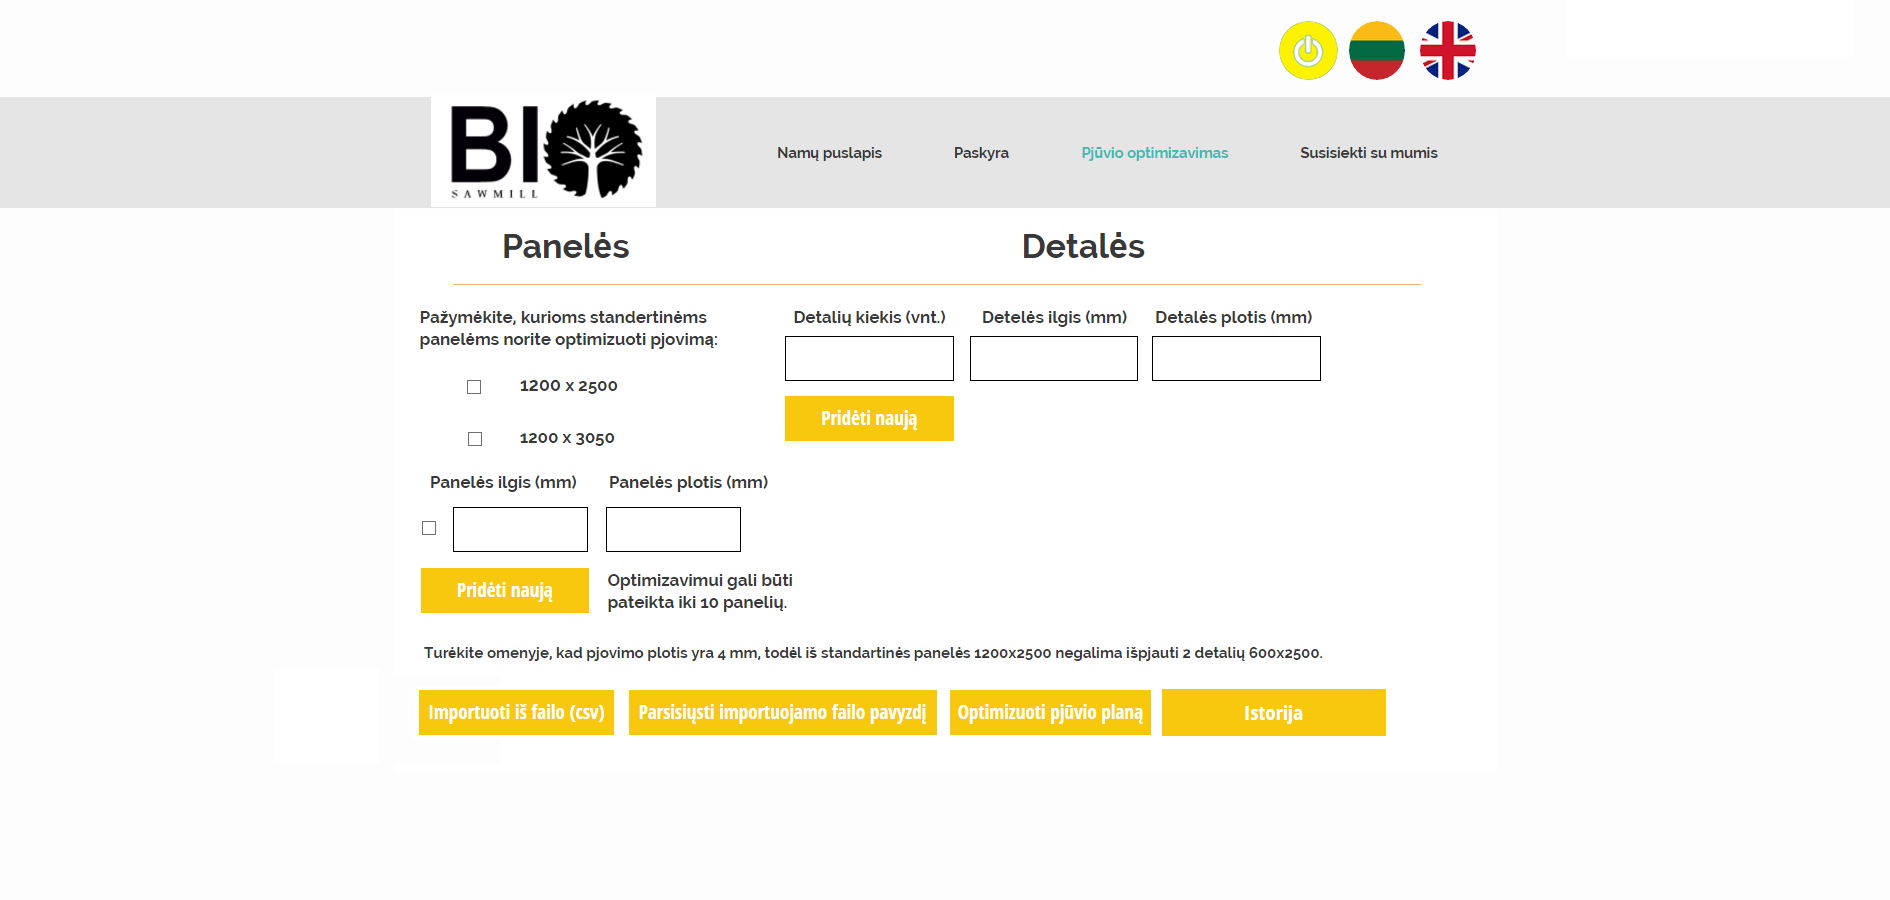
\includegraphics[scale=0.5]{interfeisai/optimizavimoPuslapisPrisijungus}

\subsection{Optimizavimo puslapis - prisijungus (su klaida)}
\hspace{-2cm}
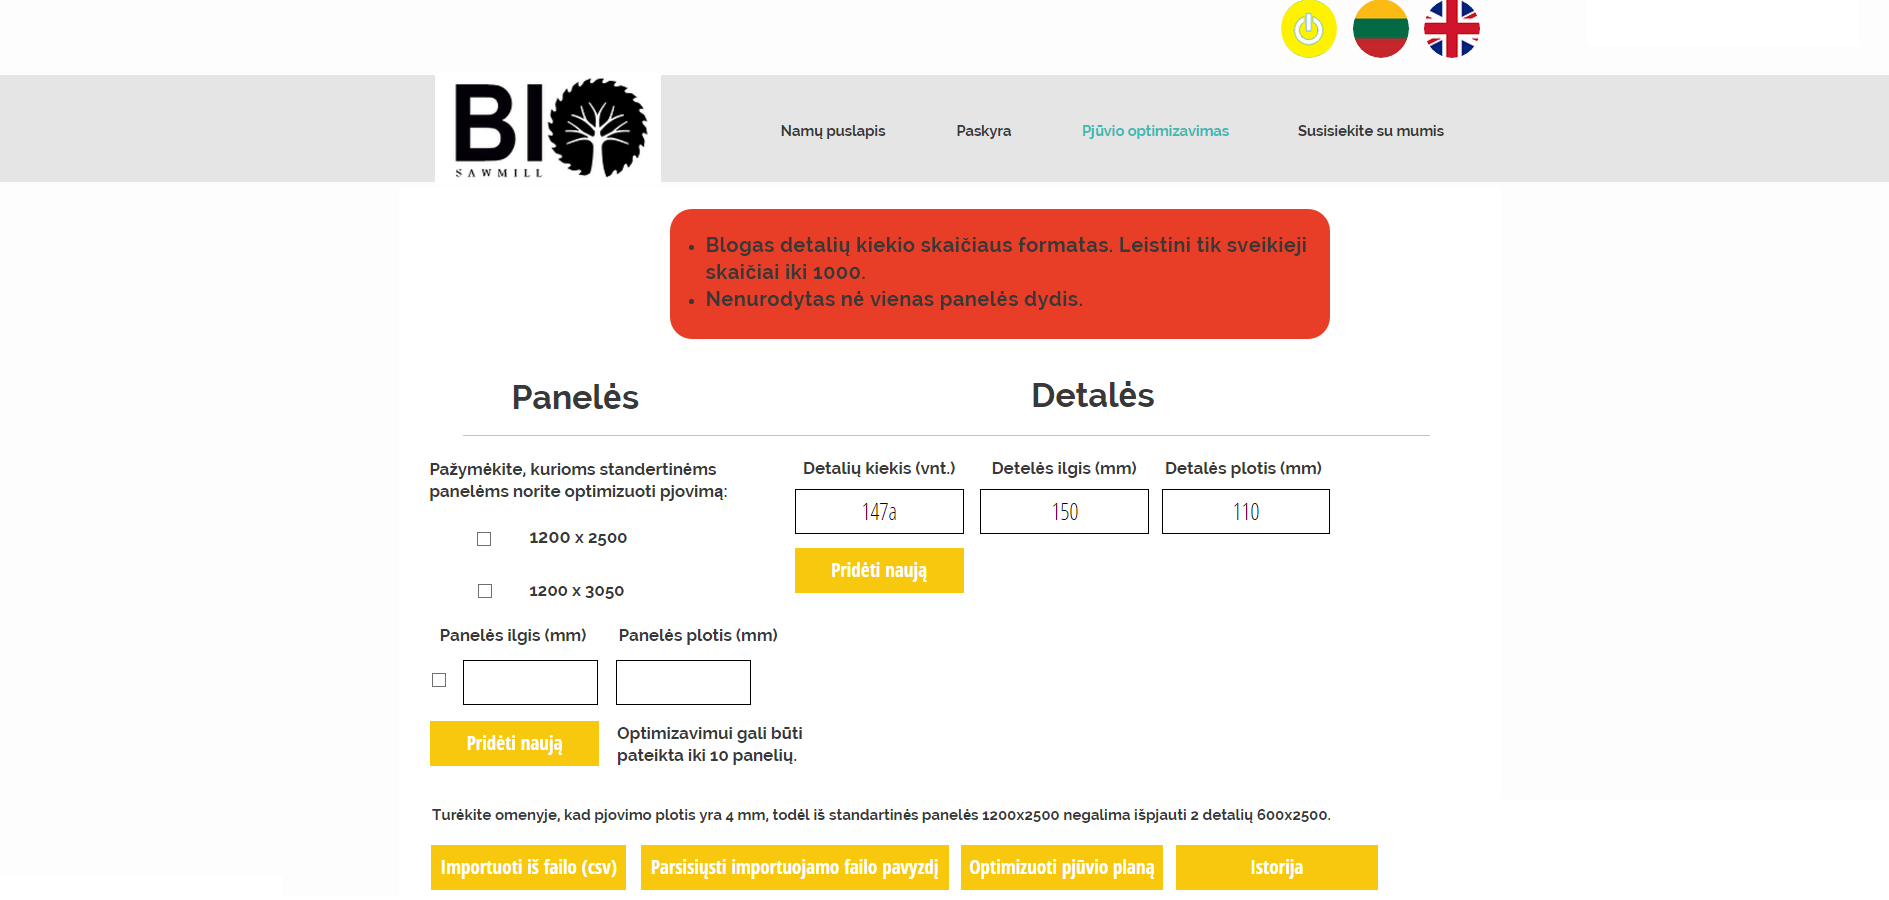
\includegraphics[scale=0.5]{interfeisai/optimizavimoPuslapisPrisijungusSuKlaida}

\subsection{Optimizavimo puslapis - po optimizavimo proceso}
\hspace{-2cm}
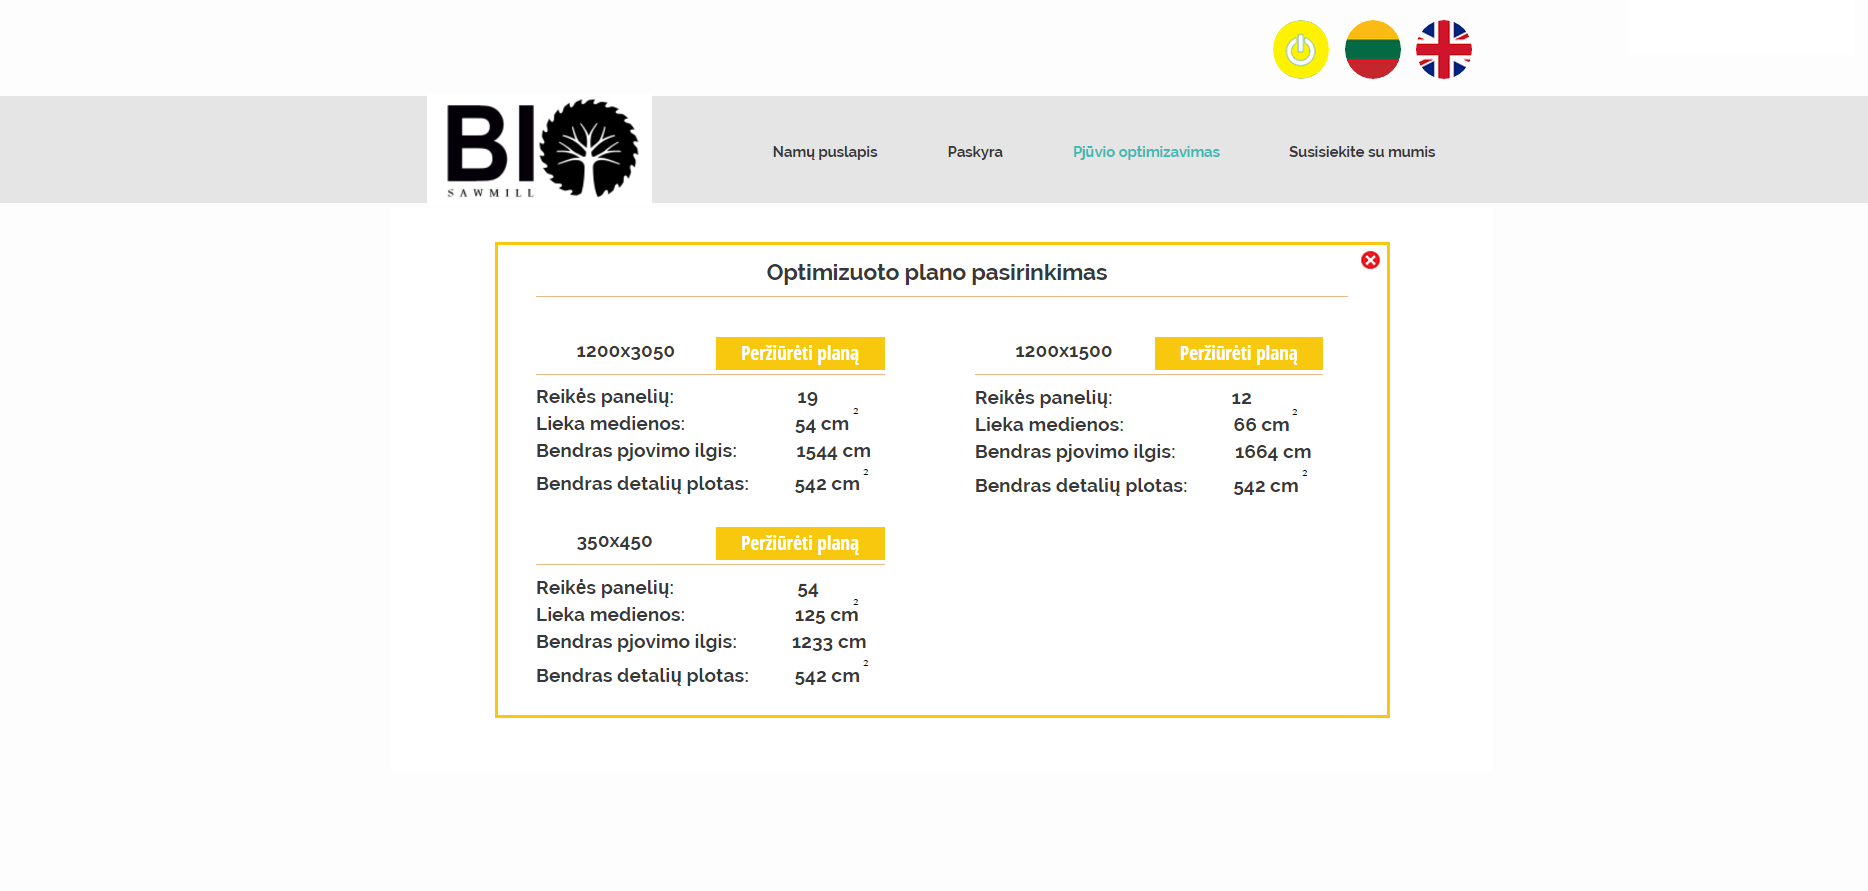
\includegraphics[scale=0.5]{interfeisai/optimizavimoPuslapisOptimizuotiPlanai}

\subsection{Optimizavimo puslapis - po optimizavimo, pasirinkus vieno iš planų peržiūrą}
\hspace{-2cm}
\includegraphics[scale=0.5]{interfeisai/optimizavimoPuslapisPrisijungusPasirinktoPerziura}

\subsection{Optimizavimo puslapis - po optimizavimo, pasirinkus vieno iš planų peržiūrą (iš arčiau)}
\hspace{-2cm}
\includegraphics[scale=1.2]{interfeisai/optimizavimoPuslapisPrisijungusPasirinktoPerziura2}

\subsection{Optimizavimo puslapis - pasirinkto plano išsaugojimas}
\hspace{-2cm}
\includegraphics[scale=0.5]{interfeisai/optimizavimoPuslapisPrisijungusPasirinktoPlanoIsaugojimas}

\subsection{Optimizavimo puslapis - pasirinkto plano išsaugojimas (su klaida)}
\hspace{-2cm}
\includegraphics[scale=0.5]{interfeisai/optimizavimoPuslapisPrisijungusPasirinktoPlanoIsaugojimasSuKlaida}

\subsection{Optimizavimo puslapis - istorijos peržiūra}
\hspace{-2cm}
\includegraphics[scale=0.5]{interfeisai/optimizavimoPuslapisPrisijungusIstorija}

\subsection{Optimizavimo puslapis - istorijos redagavimas (su klaida)}
\hspace{-2cm}
\includegraphics[scale=0.5]{interfeisai/optimizavimoPuslapisPrisijungusIstorijaSuKlaida}

\subsection{Optimizavimo puslapis - išsaugoto plano istorijoje peržiūra (iš arčiau)}
\hspace{-2cm}
\includegraphics[scale=1.2]{interfeisai/optimizavimoPuslapisPrisijungusIsaugotasPlanas}

\subsection{Susisiekimo su mumis puslapis}
\hspace{-2cm}
\includegraphics[scale=0.5]{interfeisai/susisiekimas}

\subsection{Susisiekimo su mumis puslapis (su klaida)}
\hspace{-2cm}
\includegraphics[scale=0.5]{interfeisai/susisiekimasSuKlaida}

\end{comment}
% ---------------------------------- ATKOMENTUOTA ------------------------------


\section{Klasių diagrama}


\section{Reikalavimų atsekamumų lentelė}

\end{document}
